
\chapter{Numerical Results} \label{cha: numerical results}

The numerical model described in \Cref{cha Numerical Method} was applied to simulate a simplified case of two interacting cylinders in still water ( \Cref{fig:casesetup}). The dimensional analysis (\Cref{sec:nondim}) was exploited to reduce the parameters in need of consideration. After that, I carried out mesh independence study (\Cref{sec mesh indep}) and validation (\Cref{sec validation}) to ensure the coherence between the model and the reality. At last, cylinder-interaction results (\Cref{sec results}) were produced, and found several interesting conclusions (\Cref{sec interconlude}).

%This chapter presents simulations results and analysis of them.

\section{Case Setup} \label{sec:casesetup}

The geometry of case setup is demonstrated in \Cref{fig:casesetup}. Two identical cylinders separated by distance $ G $ are immersed in still fluid. Cylinder 1 (C1) vibrates in simple harmonic motion, which is described as $ Y_1=A_1 sin(2\pi f_1t) $. Cylinder 2 (C2) is mounted to a spring, and has only 1-Degree-Of-Freedom (1DOF) along the y-axis. %The non-dimensional analysis shows that five non-dimensional groups are required to define each case (see \Cref{tablecasegroups}), while the details of non-dimensional analysis are shown in Appendix \Cref{sec:nondim}. It should be noted that, as the free stream velocity is zero, the Reynolds number $ Re_m $ is defined by the maximum velocity of C1's oscillation.

%\begin{figure}[tbp]
%	\centering
%	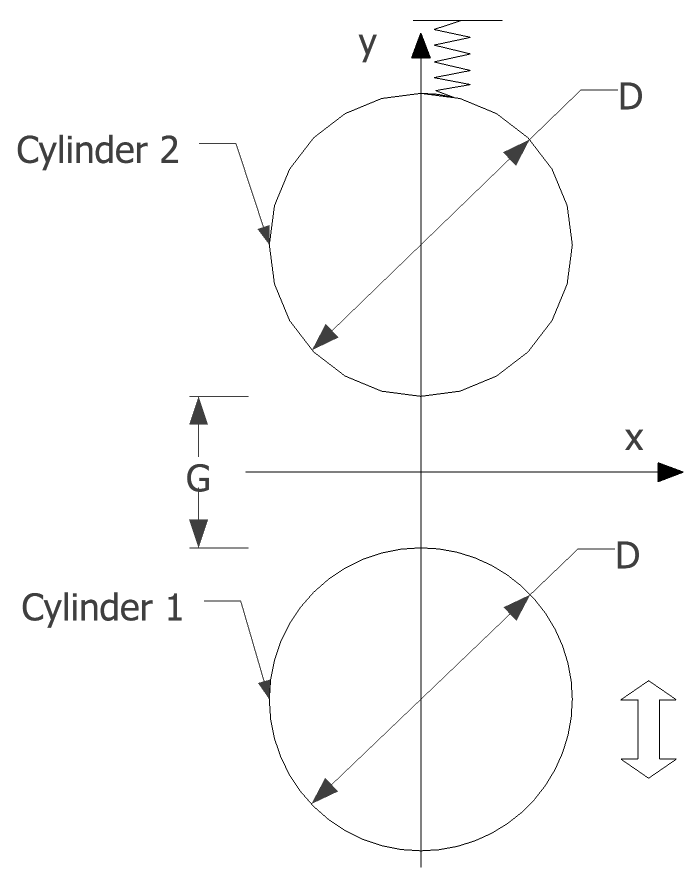
\includegraphics[width=0.5\textwidth]{Figs/Case_drawing}
%	\caption{Interaction between two cylinders: Cylinder 1 (C1) undergoes harmonic forced vibration while Cylinder 2 (C2) responds with 1DOF along y-axis with restoring force.}
%	\label{fig:casesetup}
%\end{figure}
%
%\begin{figure}[tbp]
%	\centering
%	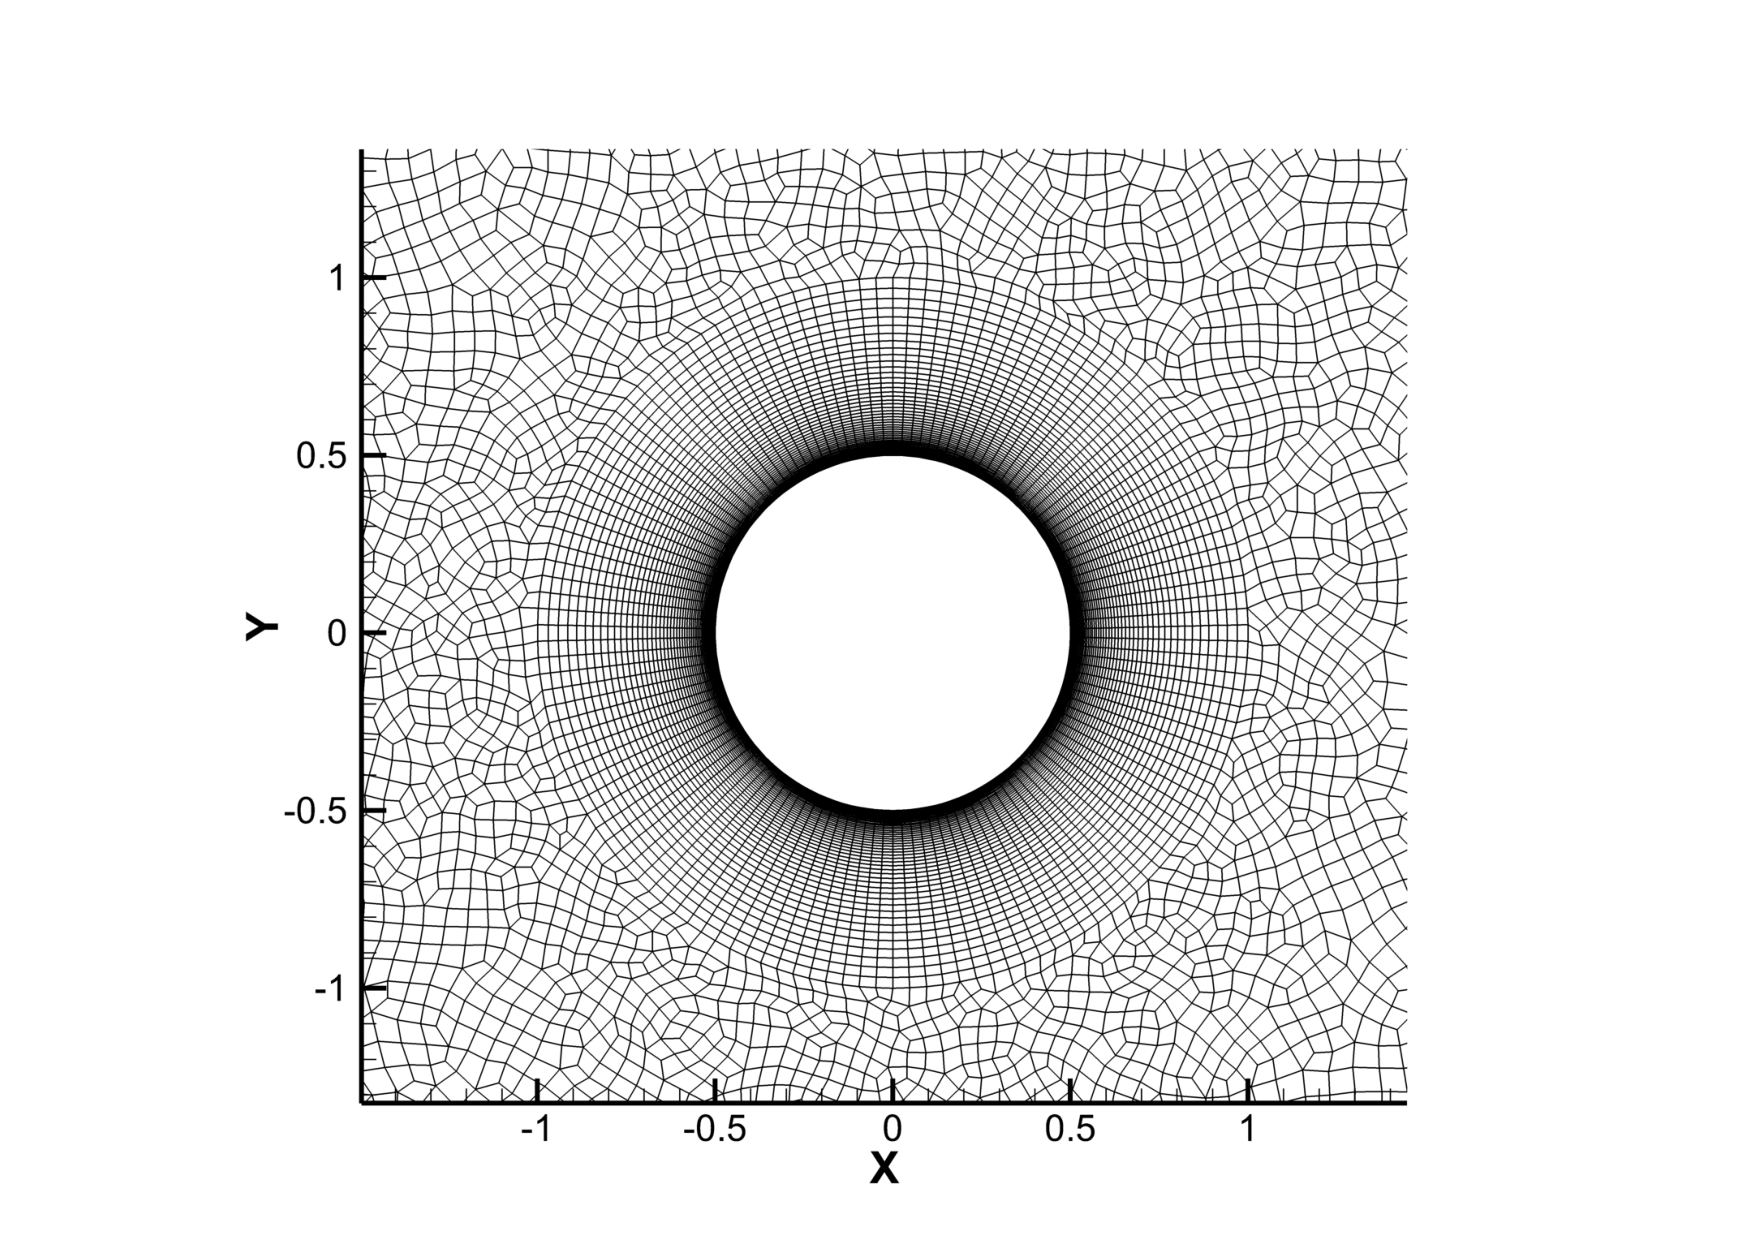
\includegraphics[width=0.8\textwidth]{Figs/single_cylinder}
%	\caption{Computational mesh around the single cylinder used for validation case}
%	\label{fig:singlecylinder}
%\end{figure}
%\begin{figure}[tbp]	
%	\centering
%	\captionsetup{justification=centering}
%	%\captionsetup[subfigure]{labelsep = none}
%	%\captionsetup[subfigure]{labelformat = empty}
%	\begin{subfigure}[t]{\textwidth}
%		\centering
%		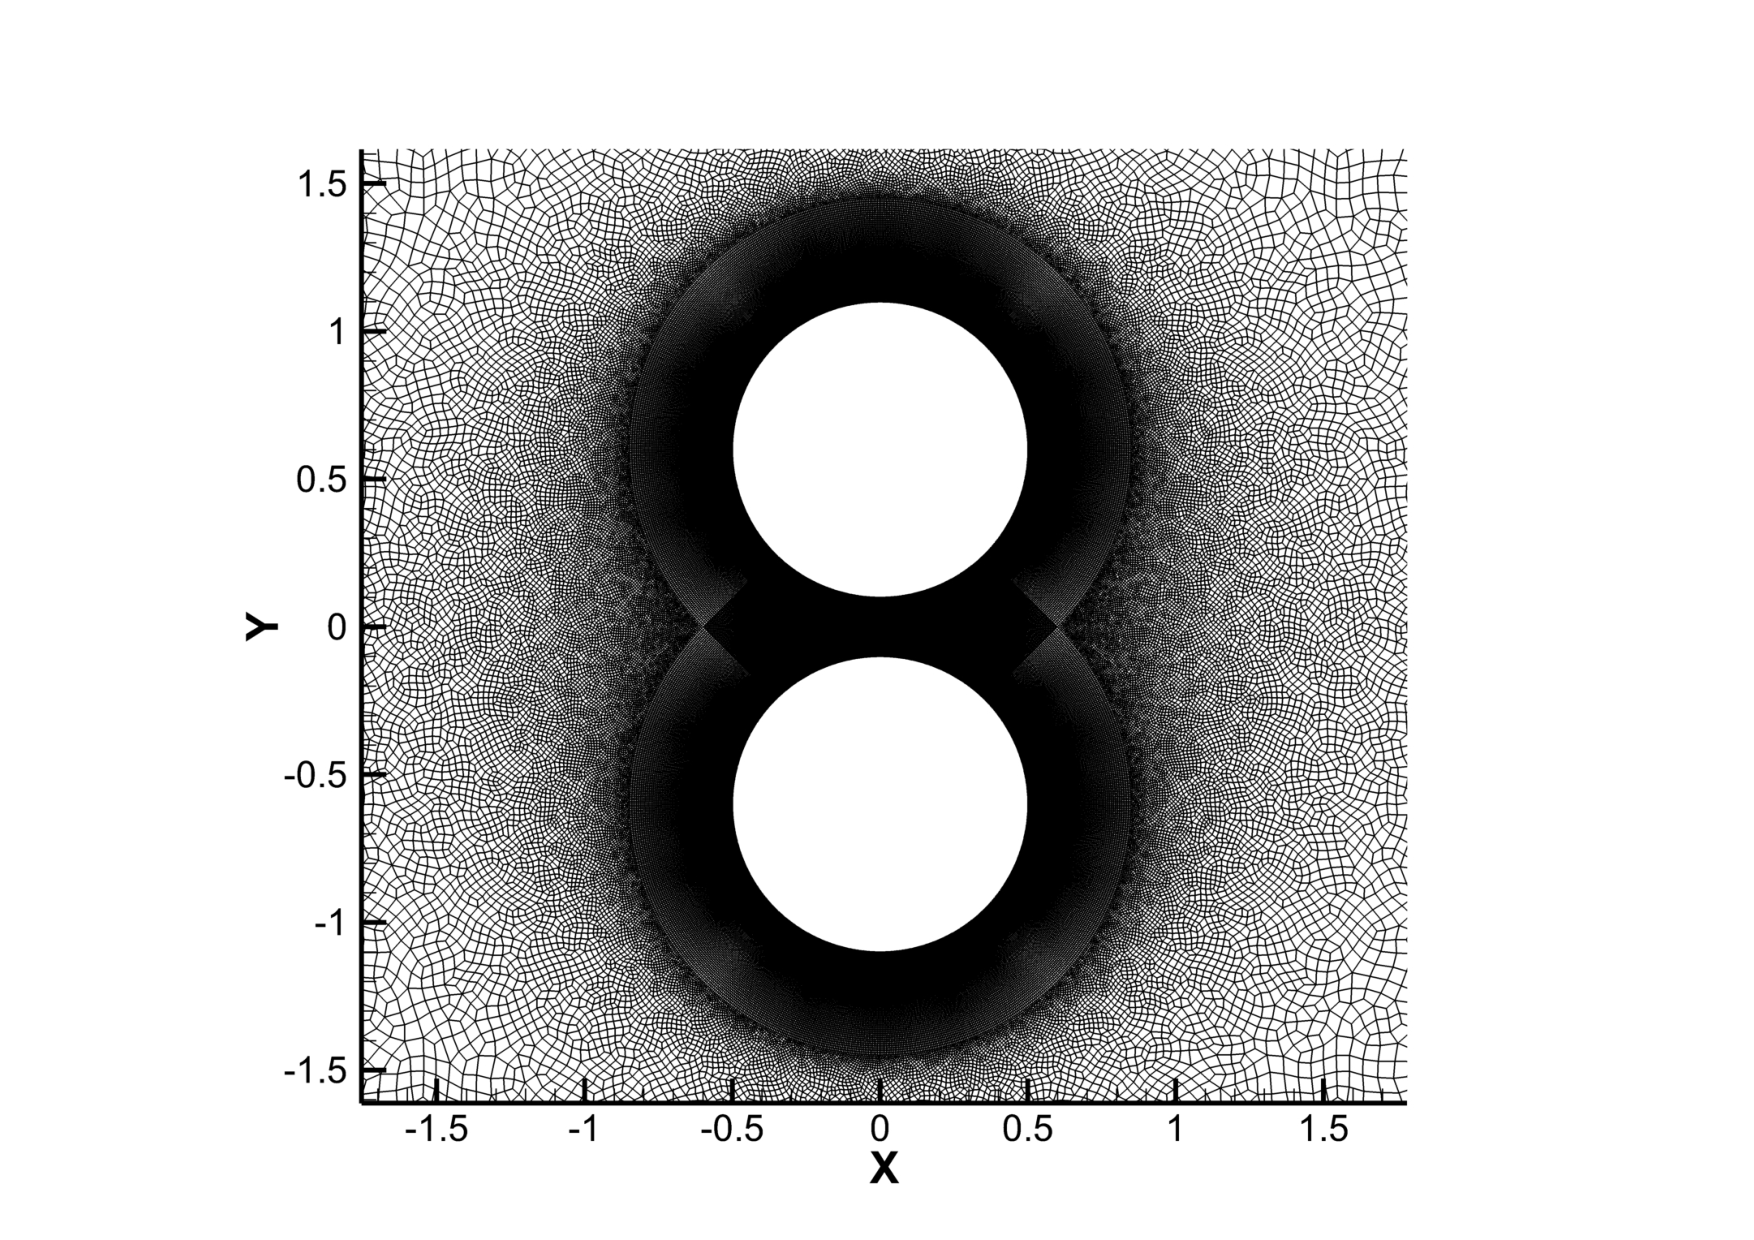
\includegraphics[width=\textwidth]{Figs/two_cylinders}
%		\caption{}
%		\label{fig:twocylinders}
%	\end{subfigure}\\%
%	\begin{subfigure}[t]{\textwidth}
%		\centering
%		\includegraphics[width=\textwidth]{"Figs/two cylinders_gap_zone"}
%		\caption{}
%		\label{fig:two-cylindersgapzone}
%	\end{subfigure}%
%	\caption{
%		Computational mesh for two cylinders with G=0.2. (a) General setting. (b) Details in the gap.
%	}
%	
%\end{figure}


\begin{figure}[tb]		
	\newcommand\widthp{0.5}
	\centering
	\captionsetup{justification=centering}
	%\captionsetup[subfigure]{labelsep = none}
	%\captionsetup[subfigure]{labelformat = empty}
		\centering
		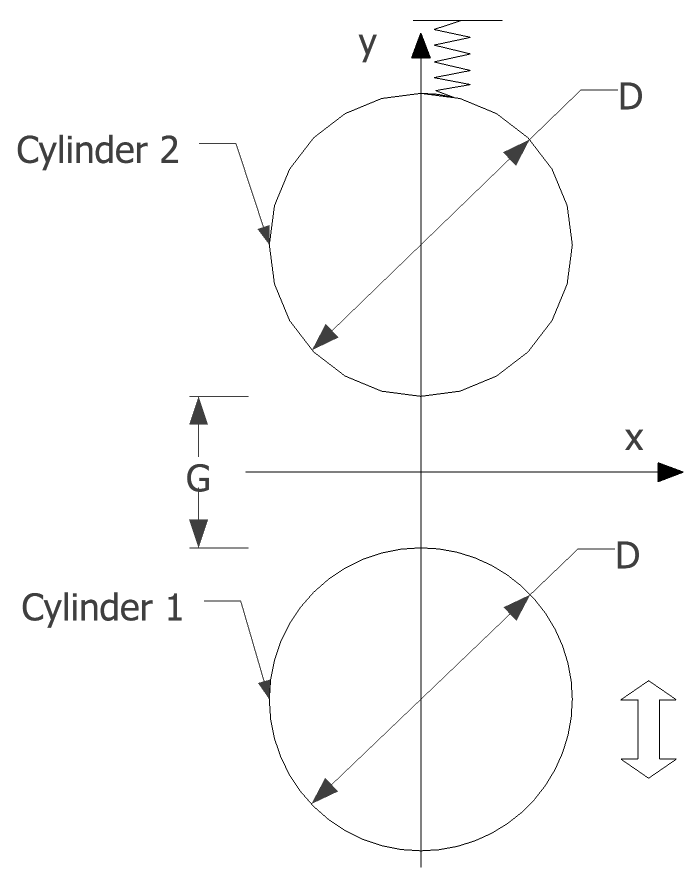
\includegraphics[width=0.4\linewidth]{Figs/Case_drawing}
	\caption{Interaction between two cylinders: Cylinder 1 (C1) undergoes harmonic forced vibration while Cylinder 2 (C2) responds with 1DOF along y-axis with restoring force. 
	}
		\label{fig:casesetup}
\end{figure}


%{==============

\section{Dimensional Analysis} \label{sec:nondim}

	%\setlength{\belowdisplayskip}{0.3pt} \setlength{\belowdisplayshortskip}{0.3pt}
	%\setlength{\abovedisplayskip}{0.3pt} \setlength{\abovedisplayshortskip}{0.3pt}
	
%	\begin{figure}[tbp]
%		\centering
%		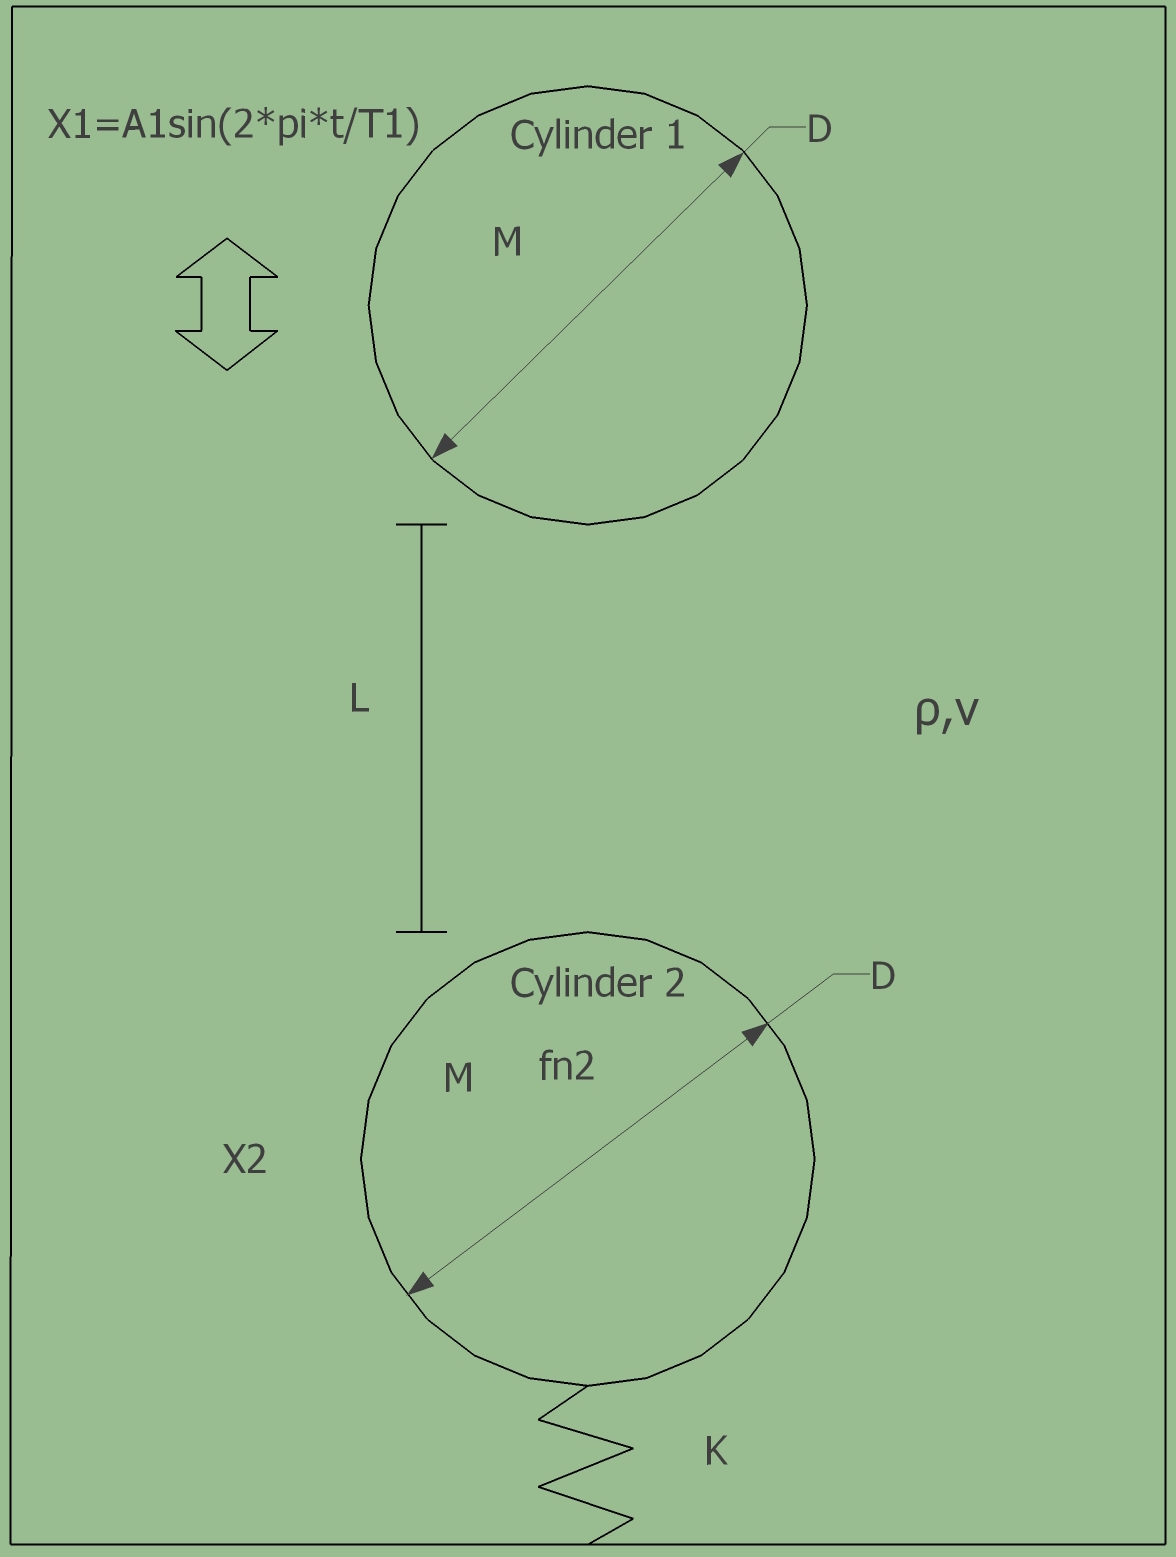
\includegraphics[width=0.7\linewidth]{Figs/nondim}
%		\caption{Scheme for case setup}
%		\label{fig:nondim}
%	\end{figure}

Dimensional analysis is a mathematical method used to predict physical parameters that influence the flow in fluid mechanics, heat transfer in thermodynamics, and so forth. The analysis involves the fundamental units of dimensions [M], [L] and [T] (i.e. mass, length, and time). It is helpful in experimental studies as it offers a guide to factors that significantly affect the studied phenomena. \cite{wiki:DimAnalysis}
%Dimensional analysis is commonly used to determine the relationships between several variables when an exact functional relationship is unknown.

For the case studied in this research (see \Cref{fig:casesetup}), Buckingham theorem is applied to find out the dimensionless groups influencing the simulation results. The procedure is as follows:

By my experience on the topic, for this case, there are 9 quantities and 3 dimensions:
	\begin{center}
		
		$\begin{bmatrix}
		D 	&  f_{n}  &  m &  \widetilde{A}_1 &  \widetilde{f}_1   &  \widetilde{G}  &  \rho   &  \nu  & \widetilde{A}_2\\  
		0	&0  			&1  	&0  			&0  		&0   &1  		&0   & 0 \\ 
		1	&0  			&0  	&1  			&0  		&1   &-2  		&2  &  1 \\
		0	&-1  			&0  	&0 			&-1 	  &0    &0  		&-1    &  0  \\
		\end{bmatrix}$
		$\begin{matrix}
		\\
		M \\
		L \\
		T \\
		\end{matrix}$
	\end{center}
where $ D $ is diameter of cylinder; $ f_{n2} =\sqrt{k/m}/2\pi $, structural natural frequency of C2 (Cylinder 2); $ m $, mass of C2; $ U_{m1}=2\pi \widetilde{A}_1 \widetilde{f}_1 $, maximum velocity of C1 (Cylinder 1); $ \widetilde{f}_1 $, vibration frequency of C1; $ \widetilde{G} $, distance between C1 and C2; $ \rho $, density of fluid; $ \widetilde{\nu} $, kinematic viscosity. $ A_{2} $, vibration amplitude of C2, is the variable I am interested in.
%The units of these parameters are based on the modern MLT system: mass, length, time. All other quantities can be expressed in terms of these basic units.

According to Buckingham theorem, these quantities can be reduced to $ 9-3=6 $ independent dimensionless groups.

If $D$, $ f_{n}  $, and $m $ are selected as repeating variables, the 6 groups can be written as follows:
	\begin{align*}
	\pi_1&=\frac{\widetilde{A}_1}{D}, &
	\pi_2&=\frac{\widetilde{f}_1}{f_{n2}}, &
	\pi_3&=\frac{\widetilde{G}}{D}, & 	
	\pi_4&=\frac{\rho}{m D^{-2}}=\frac{4}{\pi m^*}, &
	\pi_5&=\frac{\widetilde{\nu}}{f_{n} D^2}=\frac{2 \pi {A}_1 {f}_1}{Re_m},&
	\pi_6&=\frac{\widetilde{A}_2}{D}.
	\end{align*}
In other words, $ A_2 $ can be determined by 5 independent dimensionless groups: $ A_1 $, $f_1 $, $ G $, $ m^* $, $ Re_m $, as seen in \Cref{equ:nondim}:
\begin{equation}\label{equ:nondim}
\frac{\widetilde{A}_2}{D}=f(\frac{\widetilde{A}_1}{D}, \frac{\widetilde{f}_1}{f_{n2}}, \frac{\widetilde{G}}{D},  m^*, Re_m)
\end{equation}

\bgroup
\def\arraystretch{2.2}%row height stretching coefficient
\begin{table}[thb]
	\caption{Non-dimensional groups to determine a case}
	\centering
	\label{tablecasegroups}
	\begin{tabular}{l c c }
		\toprule
		%		\multirow{2}{*}{Dental measurement} & \multicolumn{2}{c}{Species I} & \multicolumn{2}{c}{Species II} \\ 
		%		\cmidrule{2-5}
		%		& mean & SD  & mean & SD  \\ 
		%		\midrule
		Mass ratio & $\mr$ & {\Large $ \frac{m}{\rho D^2 \pi /4} $}  \\
		
		Gap ratio  & $  G $ &{\Large $ \frac{\widetilde{G}}{D} $}\\
		
		Amplitude ratio of C1 & $ A_1 $ &{\Large $ \frac{\widetilde{A}_1}{D} $  }\\
		
		Frequency ratio of C1  & $f_1$ &{\Large  $ \frac{\widetilde{f}_1}{f_n} $}\\
		
		Reynolds number regarding $ U_{1m} $ & $ Re_m $ &{\Large $ \frac{ 2\pi \widetilde{A}_1 \widetilde{f}_1 D}{\nu} $}\\
		\bottomrule
	\end{tabular}
\end{table}
\egroup

\section{Mesh Independence Study} \label{sec mesh indep}

The computational domain was divided into quadrilateral 4-node finite elements; the mesh for the validation case to be discussed is shown in \Cref{fig:singlecylinder}. It has a square non-dimensional computational domain with length \& width of 60 times the diameter, thus the ratio of the cylinder diameter to the computational domain width is 1.67\%. The mesh for a configuration with two cylinders with gap ratio $ G=0.2 $ is shown in figures \Cref{twocylinderssum}, which has a square non-dimensional computational domain with length and width both equal to 160. Separate meshes were generated for situations with different initial gap ratios (see \Cref{tablemeshes}). For the current simulations, the non-dimensional time steps were chosen as $ \Delta t = 0.002D/U_{1m}= 0.002/(2\pi A_1 f_1) $. The non-dimensional viscosity was calculated as $ \nu =2\pi f_1 A_1/Re_m $. 

\begin{figure}[tb]	
	\newcommand\widthp{0.5}
	\centering
	%\captionsetup{justification=centering}
	%\captionsetup[subfigure]{labelsep = none}
	%\captionsetup[subfigure]{labelformat = empty}
	\hspace*{\fill}%
	\begin{subfigure}[t]{\widthp\textwidth}
		\centering
		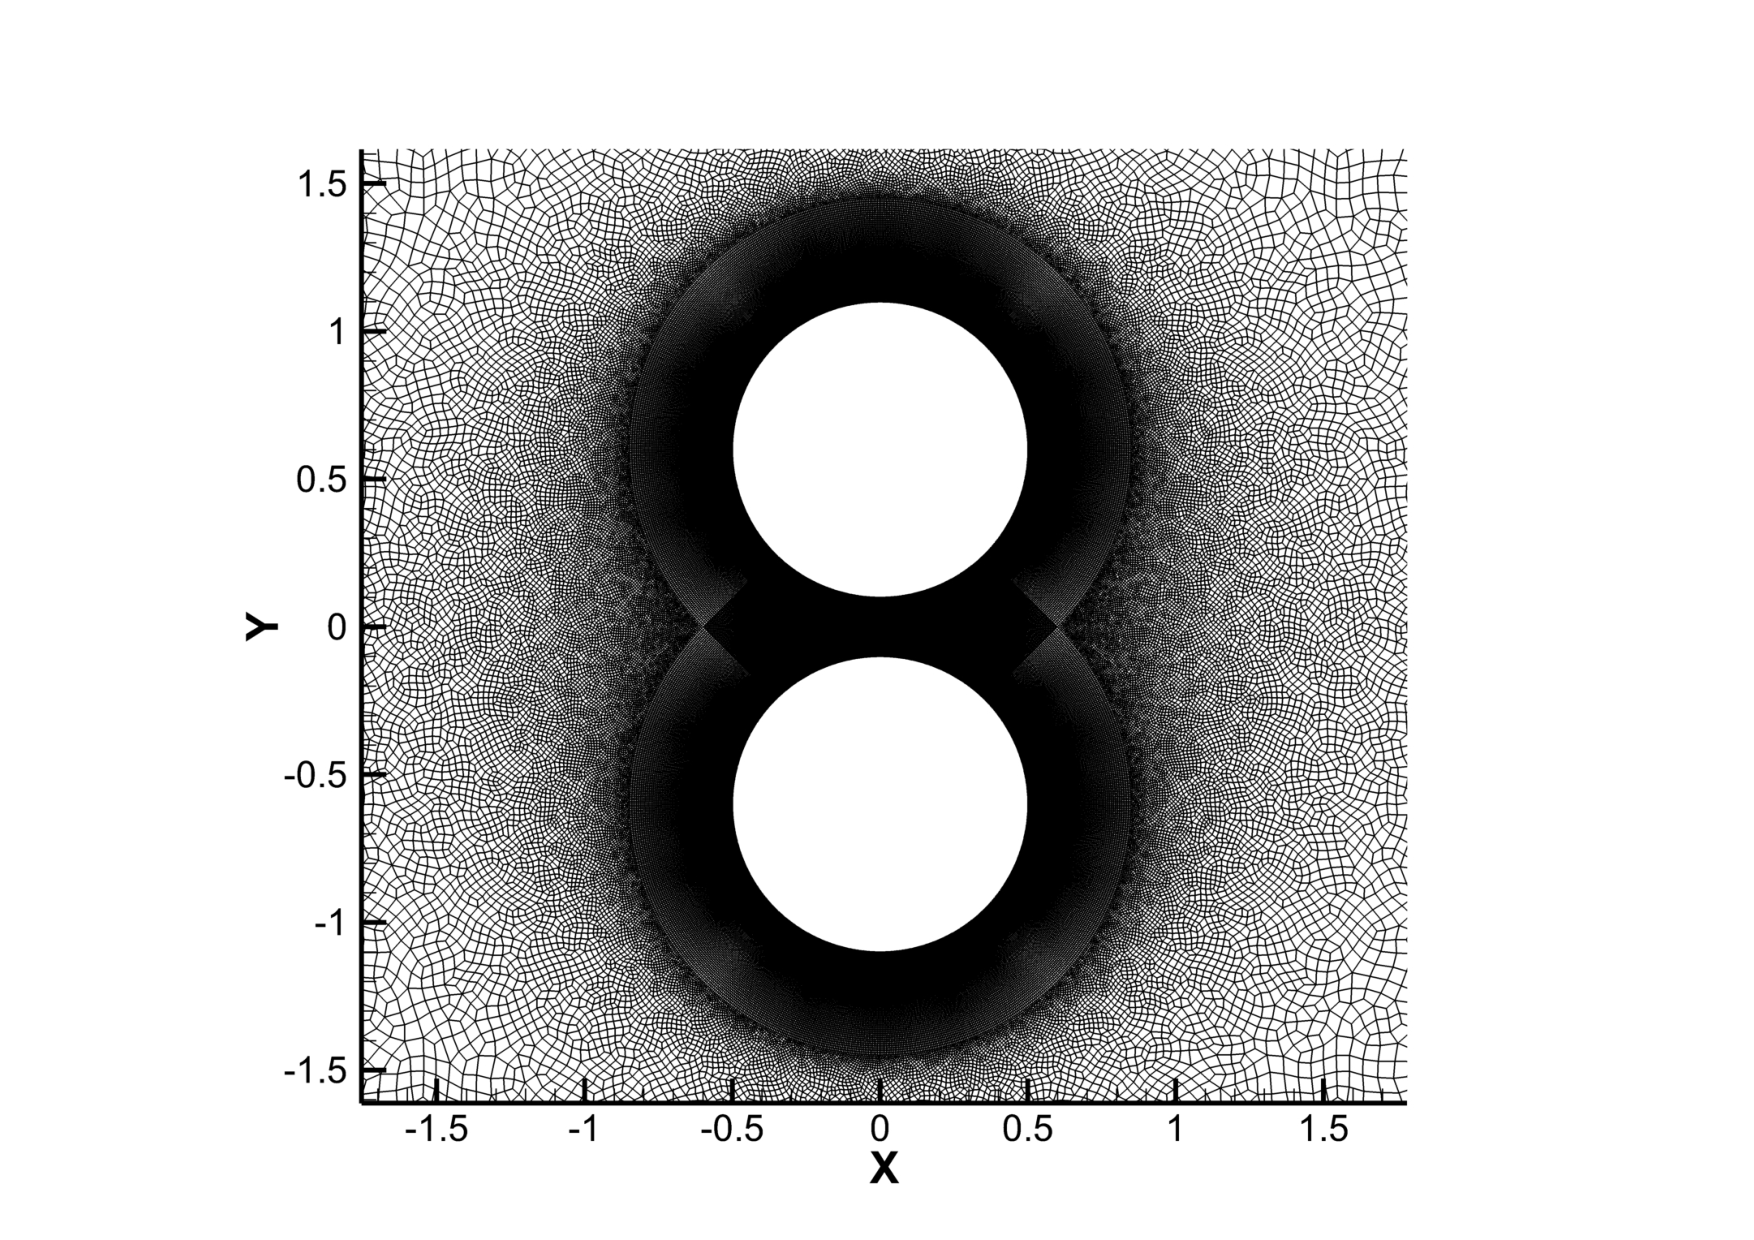
\includegraphics[width=\linewidth]{Figs/two_cylinders}
		\caption{General setting}
		\label{fig:twocylinders}
	\end{subfigure}%
	\begin{subfigure}[t]{\widthp\textwidth}
		\centering
		\includegraphics[width=\linewidth]{"Figs/two cylinders_gap_zone"}
		\caption{Details in the gap}
		\label{fig:two-cylindersgapzone}
	\end{subfigure}%
	\caption{
		Computational mesh for two cylinders with G=0.2.
	}
	\label{twocylinderssum}
	
\end{figure}

For Courant number on the radial direction, in the boundary layer near the cylinder boundary, the fluid velocity (relative to the cylinder velocity) is almost parallel to the solid surface. Therefore, the velocity in the radial direction near the cylinder surface is very small, leading to a small Courant number on the radial direction $C_r <1$. For Courant number on the circumferential direction, the number of finite elements on the circumference of the cylinder ranges from 134 to 876 (see \Cref{tablemeshes}), which means the non-dimensional element size along the circumferential direction is $ \Delta s= 0.004\sim 0.023$. As a result, the Courant number on the circumferential direction is $C_s=0.002/\Delta s \approx 0.085 \sim 0.558 <1$.



To ensure that the meshes are dense enough to produce accurate results, a mesh dependency study was conducted. The case of $ G=0.2,\ A_1=0.1,\ f_1=0.825 $ was selected for the study, because the vibration in this case has the greatest $ A_2/A_1 $. A series of meshes with various $ N_c $ (i.e.\ element number along each cylinder surface) and $ \Delta r_{min} $ (i.e.\ minimum non-dimensional element size on the radial direction of the mesh) was simulated for this case. The frequency of C2 remained constant ($ f_2=f_1=0.825 $) with the variation of $ N_c\ \&\ \Delta r $, yet the amplitude of C2 slightly changed, as seen in \Cref{fig:nca2}. It can be seen in \Cref{fig:meshindep} that, at $ \Delta r_{min} =0.000902 $ \& $ 116 \leq N_c \leq 266 $, $ A_2 $ slightly varies by $ 0.113\% $ and converges at $N_c \geq 266 $. \Cref{fig:rmina2} shows that $ A_2 $ converges with the decrease of $ \Delta r_{min} $ and varies for a mere $ 3\% $, at $ N_c=296 $ \& $ 0.00105\leq \Delta r_{min} \leq 0.0045$. For all the applied meshes (see \Cref{tablemeshes}), $ \Delta r_{min}$ was less than 0.0045 and the $ N_c $ was larger than 144. In other words, the applied meshes are dense enough for the simulations. 





\begin{table} [tb]
	\centering
	\caption{Computational meshes for various gap ratios}
	\label{tablemeshes}
	{\renewcommand{\arraystretch}{1.2}
		\begin{tabular}{|c|c|c|c|c|} \hline 
			G & \Centerstack{Total\\nodes} &\Centerstack{Nodes along\\two cylinders} & \Centerstack{Nodes along\\each cylinder} & \Centerstack{Length of\\square boundary}\\ \hline 
			Single  & 55 159 & N/A & 134 & 60 \\ \hline 
			3.00 & 136 711 & 384 & 192 & 160 \\ \hline 
			1.25 & 129 295 & 384 & 192 & 160 \\ \hline 
			1.00 & 127 791 & 288 & 144 & 160 \\ \hline 
			0.50 & 178 437 & 952 & 476 & 160 \\ \hline 
			0.40 & 170 129 & 952 & 476 & 160 \\ \hline 
			0.30 & 180 299 & 952 & 476 & 160 \\ \hline 
			0.20 & 242 329 & 1752 & 876 & 160 \\ \hline 
			0.10 & 183 599 & 952 & 476 & 160 \\ \hline 
			0.05 & 131 746 & 952 & 476 & 160 \\ \hline 
		\end{tabular}
	}
\end{table}


\begin{figure}[tbh]	
	\newcommand\widthp{0.5}
	\centering
	%\captionsetup{justification=centering}
	%\captionsetup[subfigure]{labelsep = none}
	%\captionsetup[subfigure]{labelformat = empty}
	\hspace*{\fill}%
	\begin{subfigure}[t]{\widthp\textwidth}
		\centering
		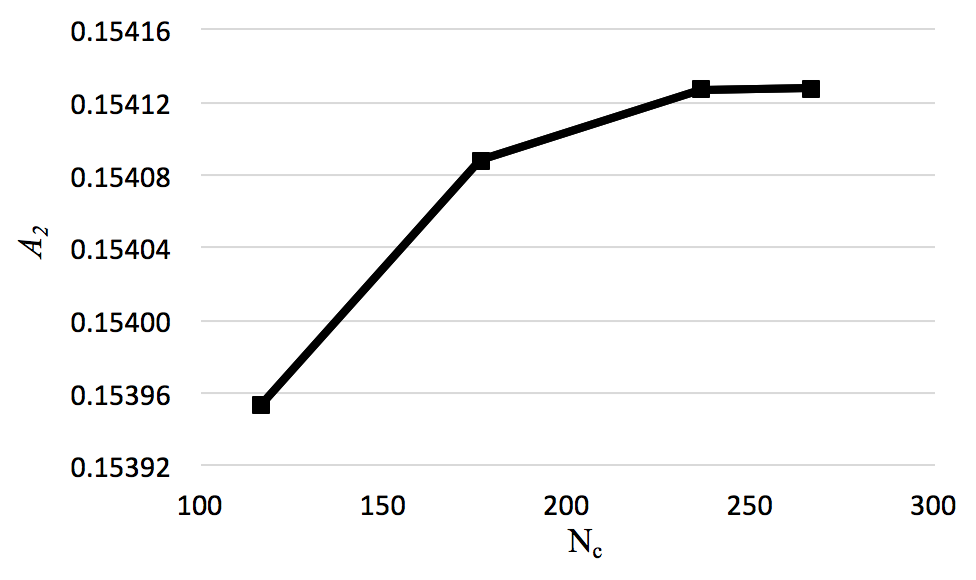
\includegraphics[width=\linewidth]{Figs/NcA2}
		\caption{effect of $ N_c $ on $ A_2 $ with $ \Delta r_{min} =0.000902$}
		\label{fig:nca2}
	\end{subfigure}%
	\begin{subfigure}[t]{\widthp\textwidth}
		\centering
		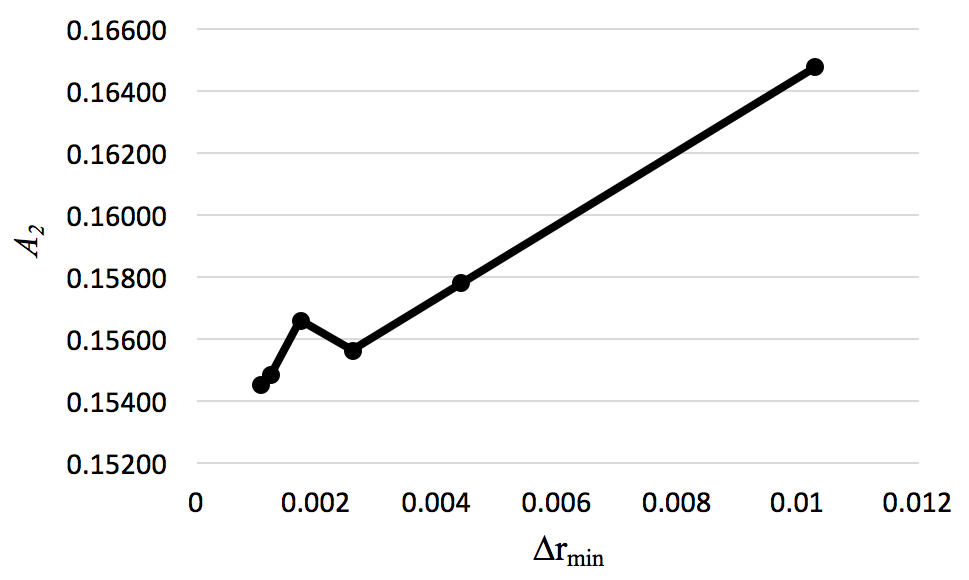
\includegraphics[width=\linewidth]{Figs/rminA2}
		\caption{effect of $ \Delta r_{min} $ on $ A_2 $ with $  N_c=296$}
		\label{fig:rmina2}
	\end{subfigure}%
	\caption{ The results of the mesh dependency study. 
	}
	\label{fig:meshindep}
\end{figure}



\section{Validation} \label{sec validation}
The validation case was set to be a single cylinder (see \Cref{fig:singlecylinder} and \Cref{tablemeshes}) oscillating harmonically in still fluid at $KC=U_{max}/(fD)=5$, $Re_m=U_mD/\nu =100$. The simulation results were compared with the experimental data obtained by Dutsch \cite{DUTSCH1998}, as seen in \Cref{fig:validation}. The horizontal \& vertical velocity components ($u$ \& $v$) of the predicted and measured data are compared along $y/D$ = 0.6, 0, -0.6 and -1.2 for phases $\psi =180^{\circ}$, $210^{\circ}$, $330^{\circ}$. In \Cref{fig:validation}, the lines represent the simulation results, while symbols stand for experimental data. It can be seen that the simulation results match with the experimental data well. In addition, the applied numerical model has been validated in several VIV-studies \cite{Zhao2013,Cui2014,Zhao2014,Zhao2013e}.
\begin{figure}[hb!]
		\centering
		\captionsetup{justification=centering}
		\includegraphics[width=0.40\linewidth]{"Figs/single_cylinder"}
		\caption{Single cylinder mesh for validation case with $ N_c=134 $ and $ \Delta r\approx0.00183 $}
		\label{fig:singlecylinder}
\end{figure}

\begin{figure}[tbp]
	\centering
	\captionsetup{justification=centering}
	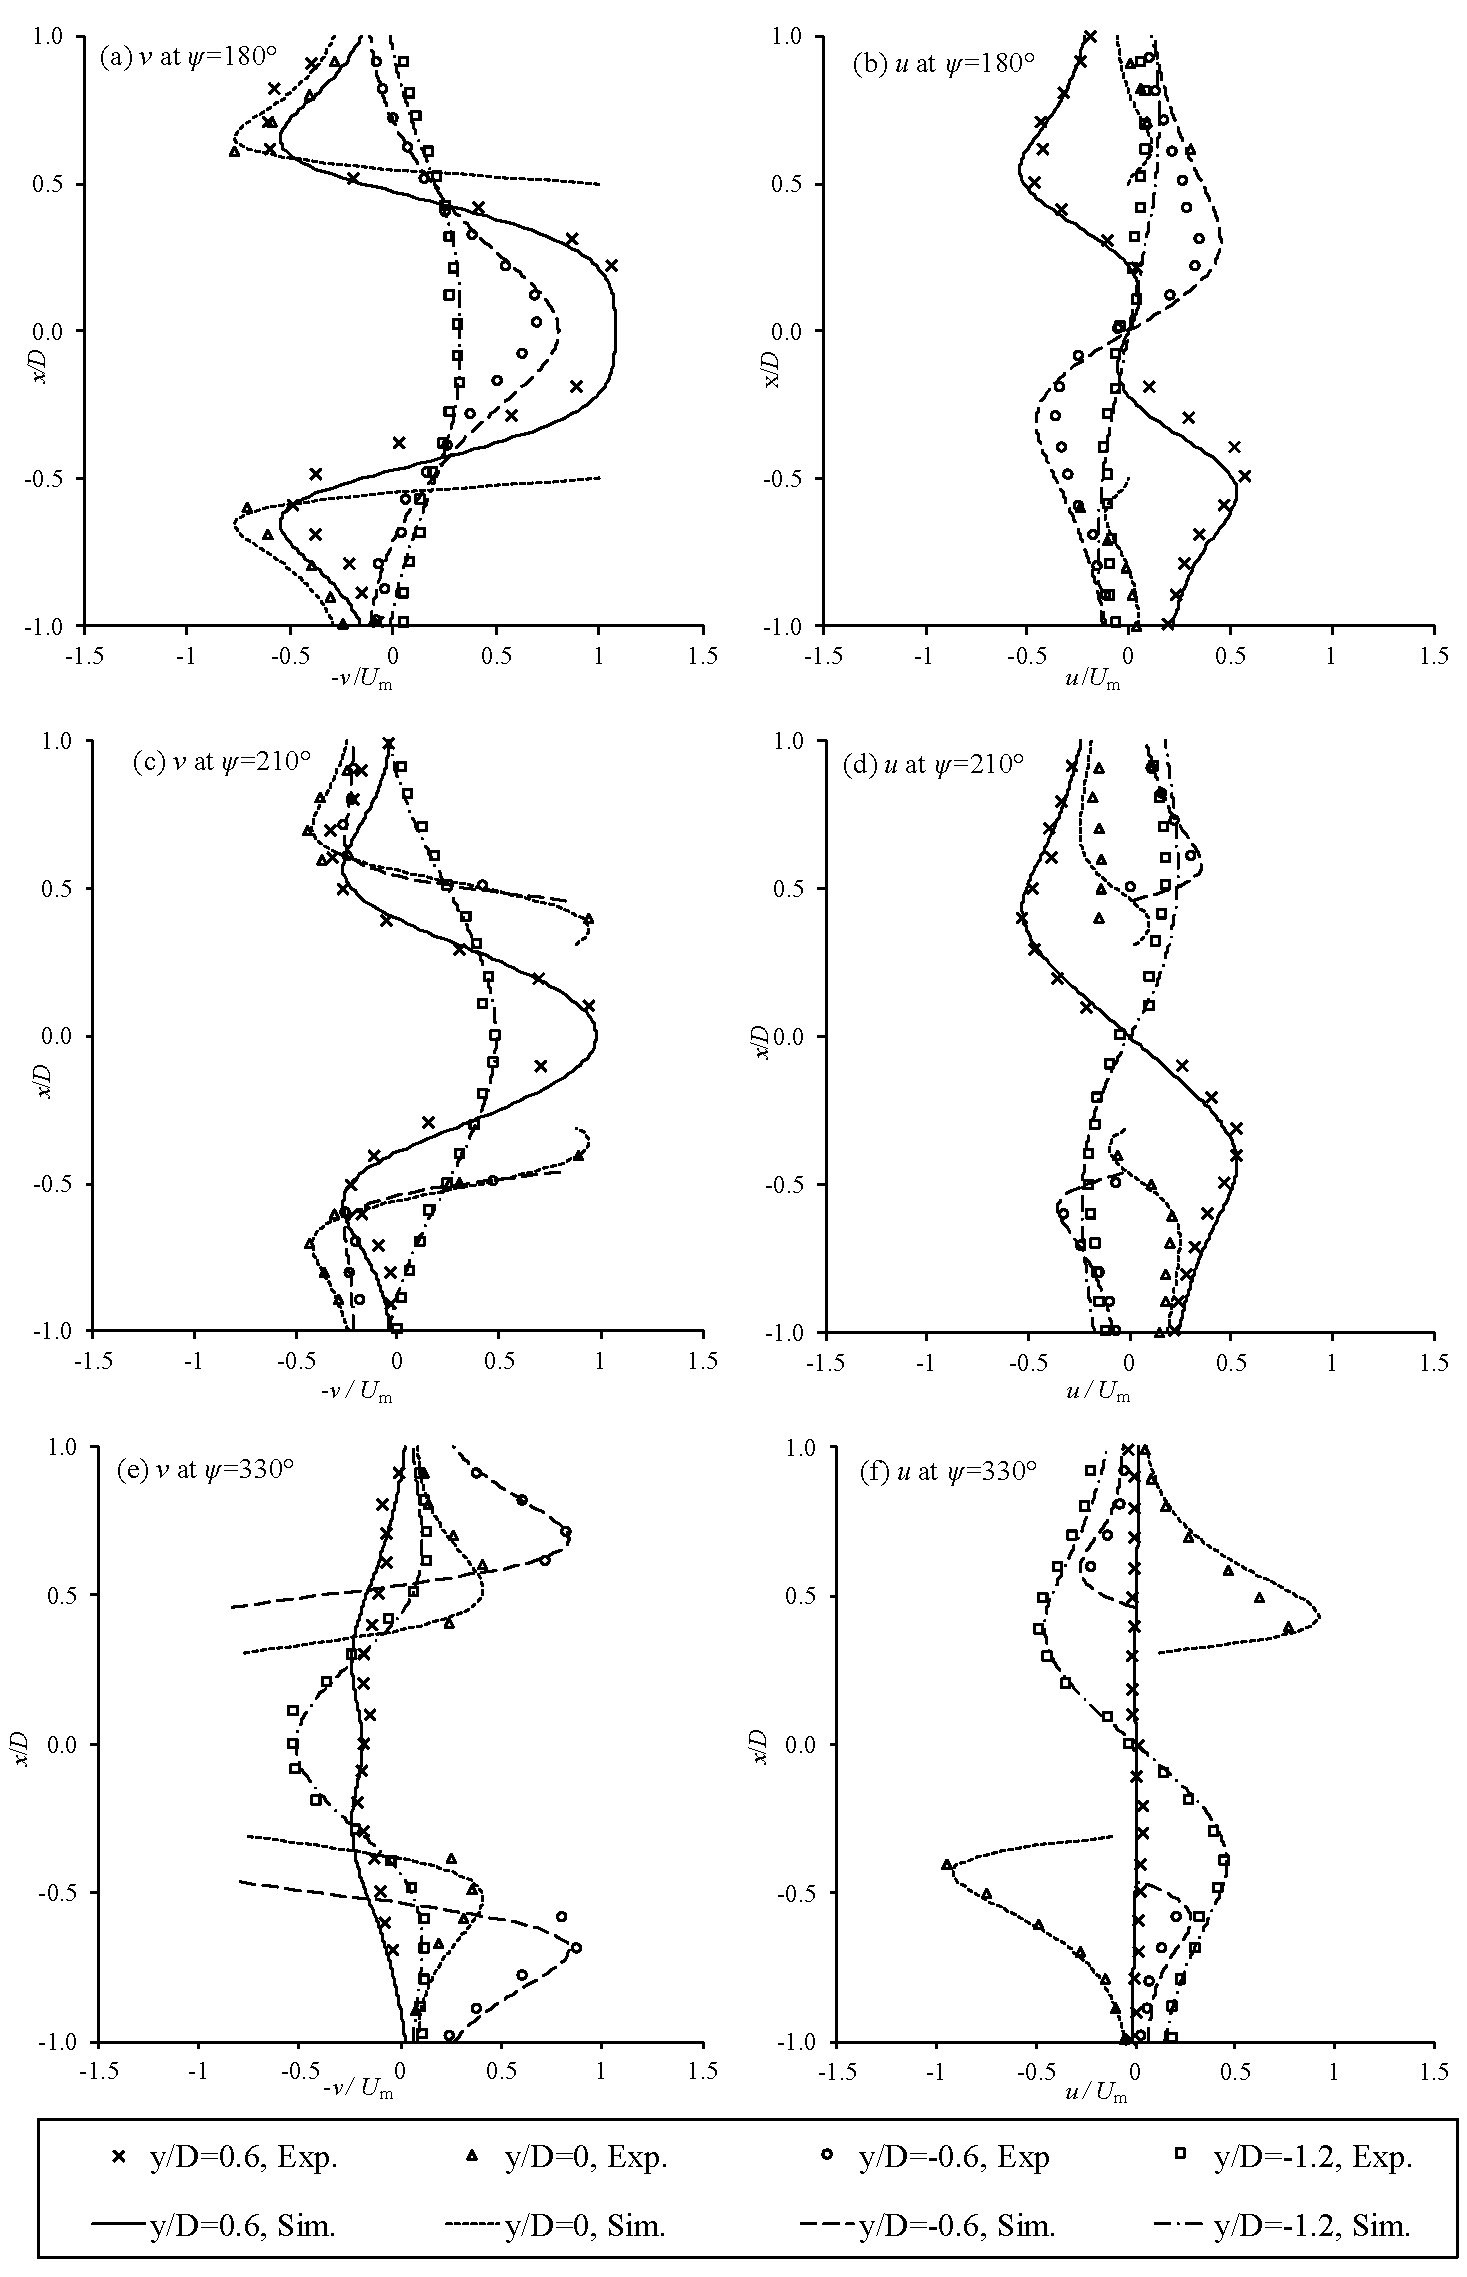
\includegraphics[height=\textheight]{Figs/validation}
	\caption{Comparison of fluid velocity distribution between the numerical simulation results and the experimental data by Dutsch \cite{DUTSCH1998}}
	\label{fig:validation}
	\captionsetup{justification=centering}
\end{figure}


% **************************** Define Graphics Path **************************
 \graphicspath{{Figs/}}

%T: f1=f2 ? check again, search for code online


\clearpage

\section{Cylinder-interaction Results} \label{sec results}

As Cylinder 1 (C1) experiences forced vibration, the surrounding fluid is disturbed, generating vortices around C1. The disturbed fluid induces the vibration of Cylinder 2 (C2), which also generates its own vortices. The vortices adjacent to C1 and C2 interact with one another, lending extra complication to the situation. 

The interaction between C1 and C2 was simulated with a series of initial gap ratios G, such that $G=0.025 \sim3$.  C1's forced vibrational amplitude was configured to be smaller than the corresponding gap ratio to avoid collision between cylinders, and C1's non-dimensional frequency ranges from 0.05 to 2.4.


%The interaction between C1 and C2 has been simulated with 9 initial gap ratios $ G $, such that $ G\in \[0.025, 3\]$.  C1's forced vibration amplitude was configured to be smaller than the corresponding gap ratio to avoid collision between cylinders, and C1's non-dimensional frequency ranges from 0.05 to 2.4. The study of the interaction between two cylinders mainly focused on the C2's amplitude, $ A_2 $.

For all the cases simulated, the frequency of C2 was identical to C1 ($f_1=f_2  $), as seen in \Cref{fig:freqcheck}. In addition, it is interesting that, as $ f_1 $ increased from 0.05 to 2.5, the motion of C1 and C2 gradually changed from being in anti-phase (see \Cref{fig:freq0.65}) to being in phase (see \Cref{fig:freq2.0}), and $ A_2 $ reaches maximum when $ f_1 $ is slightly less than the critical value (around 0.8) between in anti-phase and in phase. After $ A_2 $ reaches maximum, the motion of C1 and C2 remains in phase (see \Cref{fig:freq1.6,fig:freq2.0}). 

\begin{figure}[tbp]	
	\newcommand\widthp{0.5}
	\centering
	\captionsetup{justification=centering}
	%\captionsetup[subfigure]{labelsep = none}
	%\captionsetup[subfigure]{labelformat = empty}
	\hspace*{\fill}%
	\begin{subfigure}[t]{\widthp\textwidth}
		\centering
		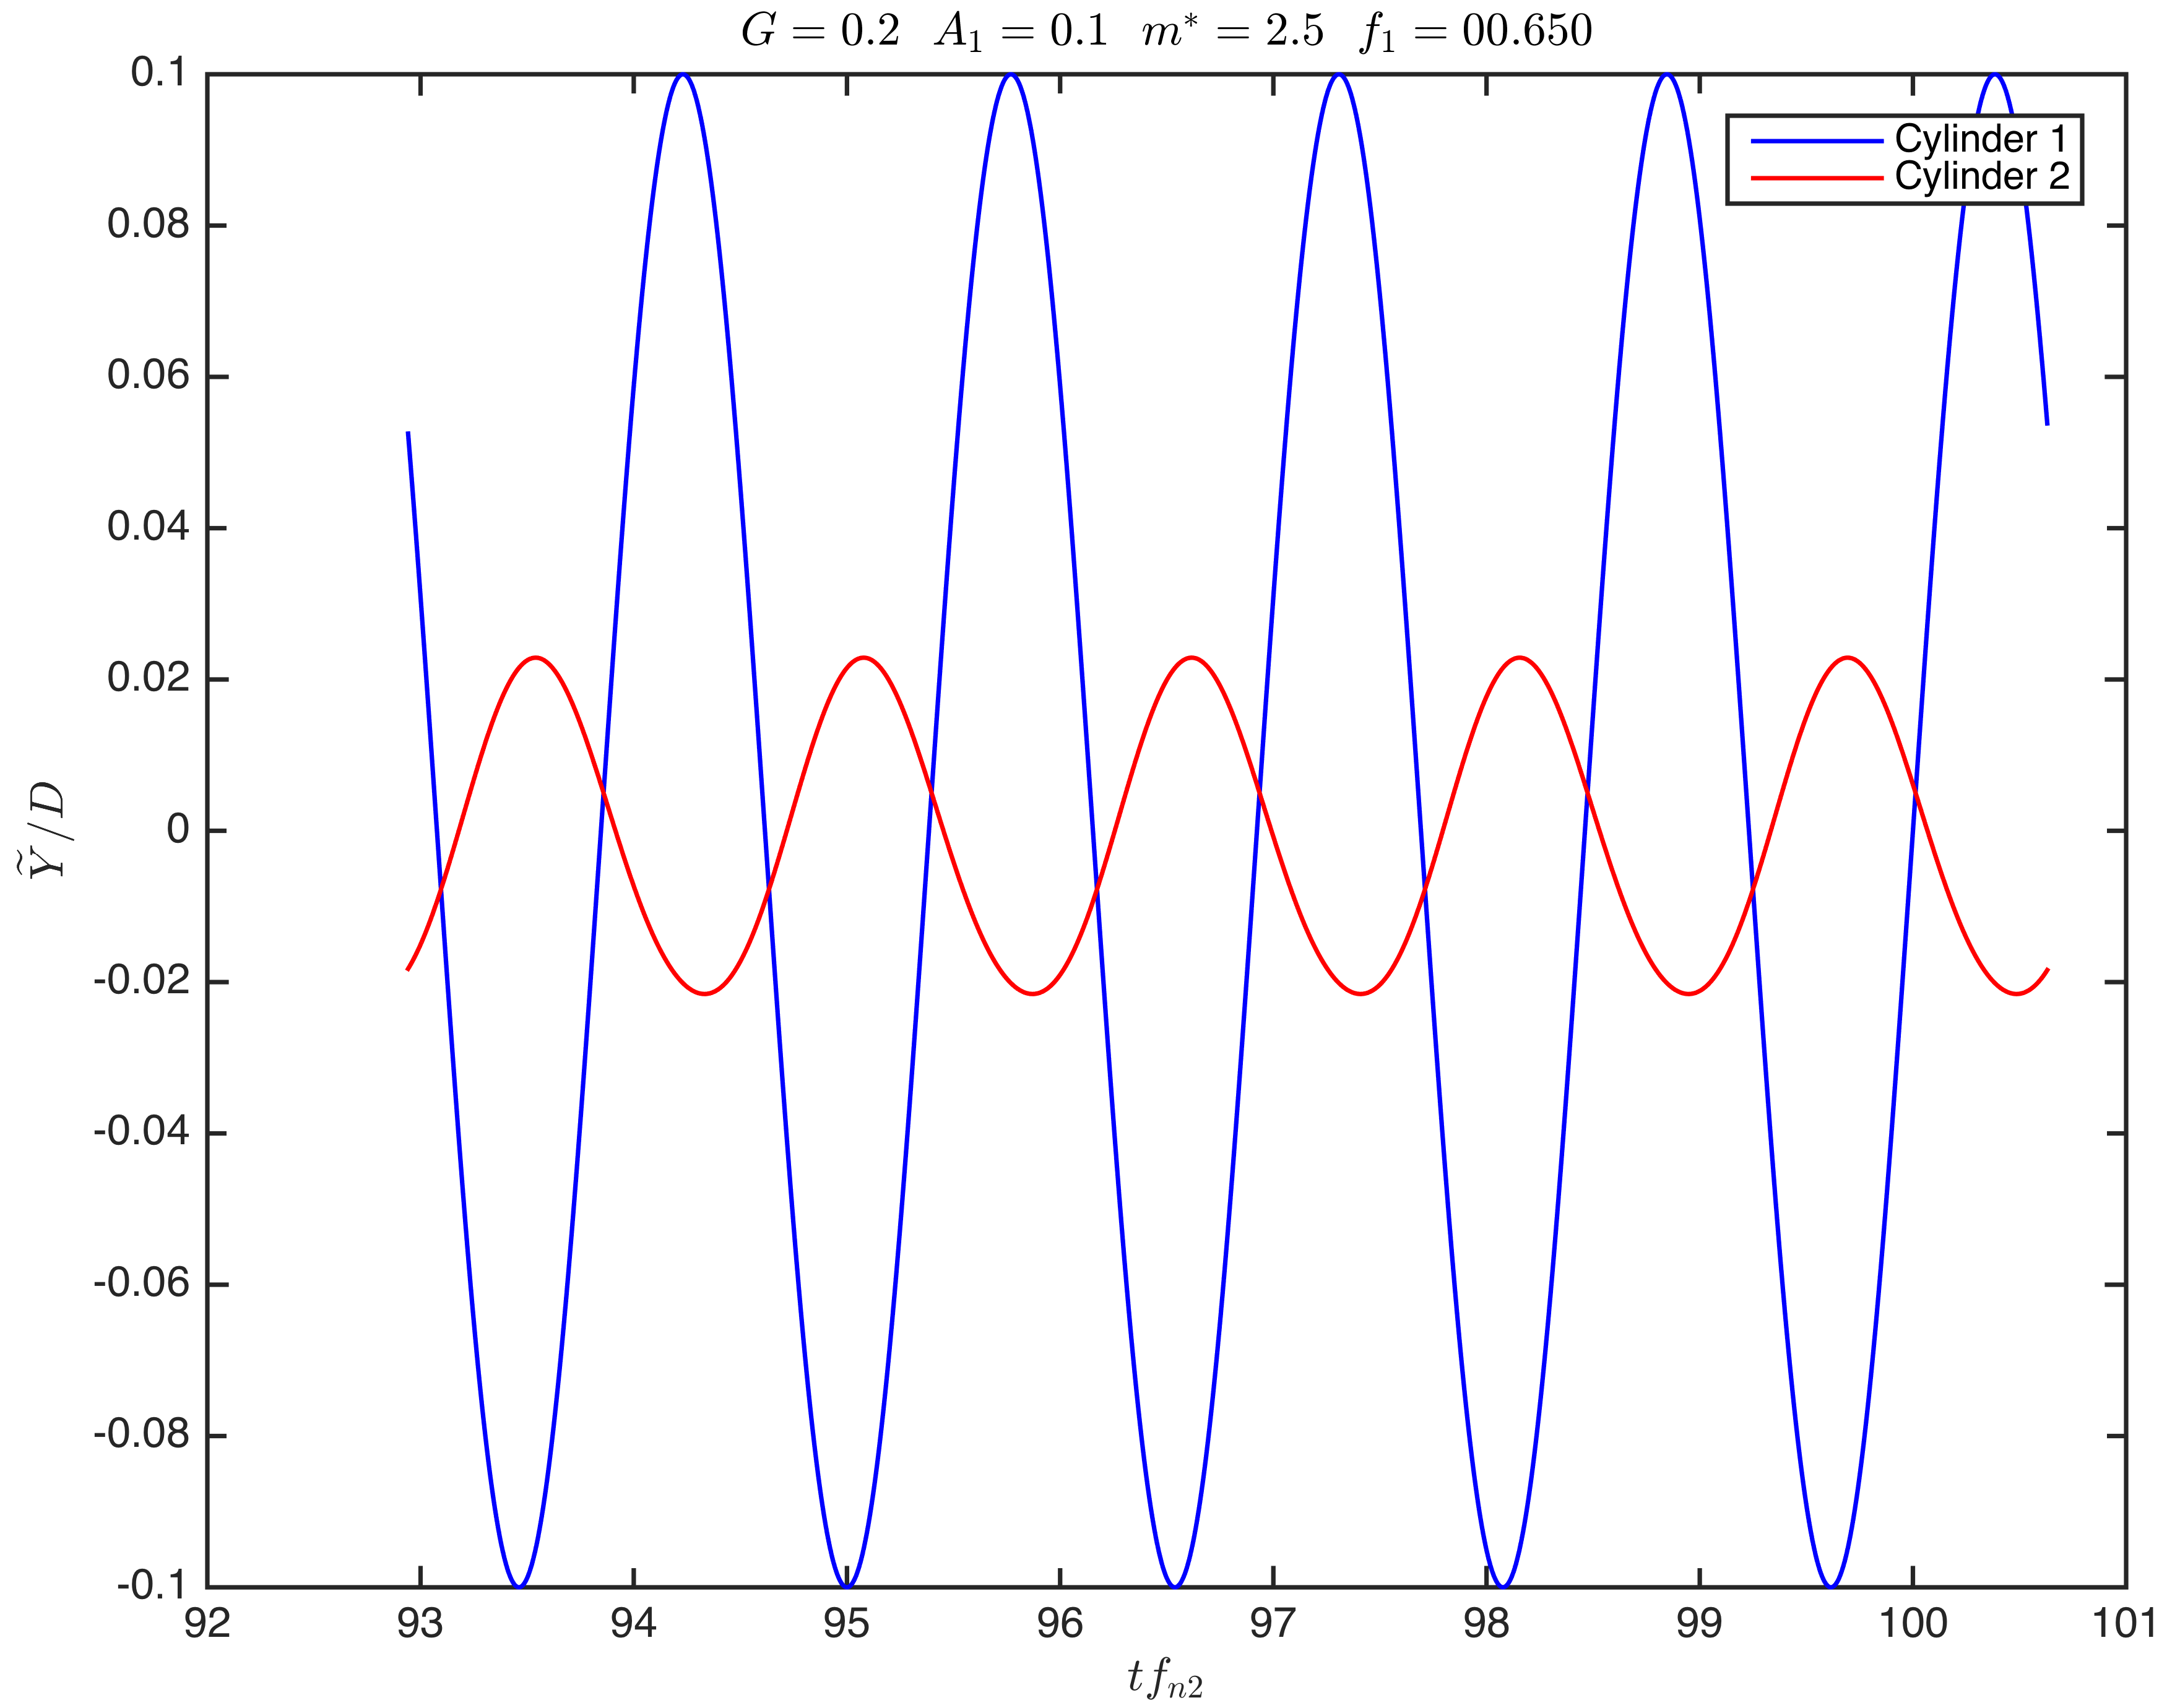
\includegraphics[width=1\linewidth]{Figs/Plotting_g0.20a0.100m2.5zl_r48_00.650_VIV02}
		\caption{$ f_1=0.65 $, anti-phase}
		\label{fig:freq0.65}
	\end{subfigure}%
	\begin{subfigure}[t]{\widthp\textwidth}
		\centering
		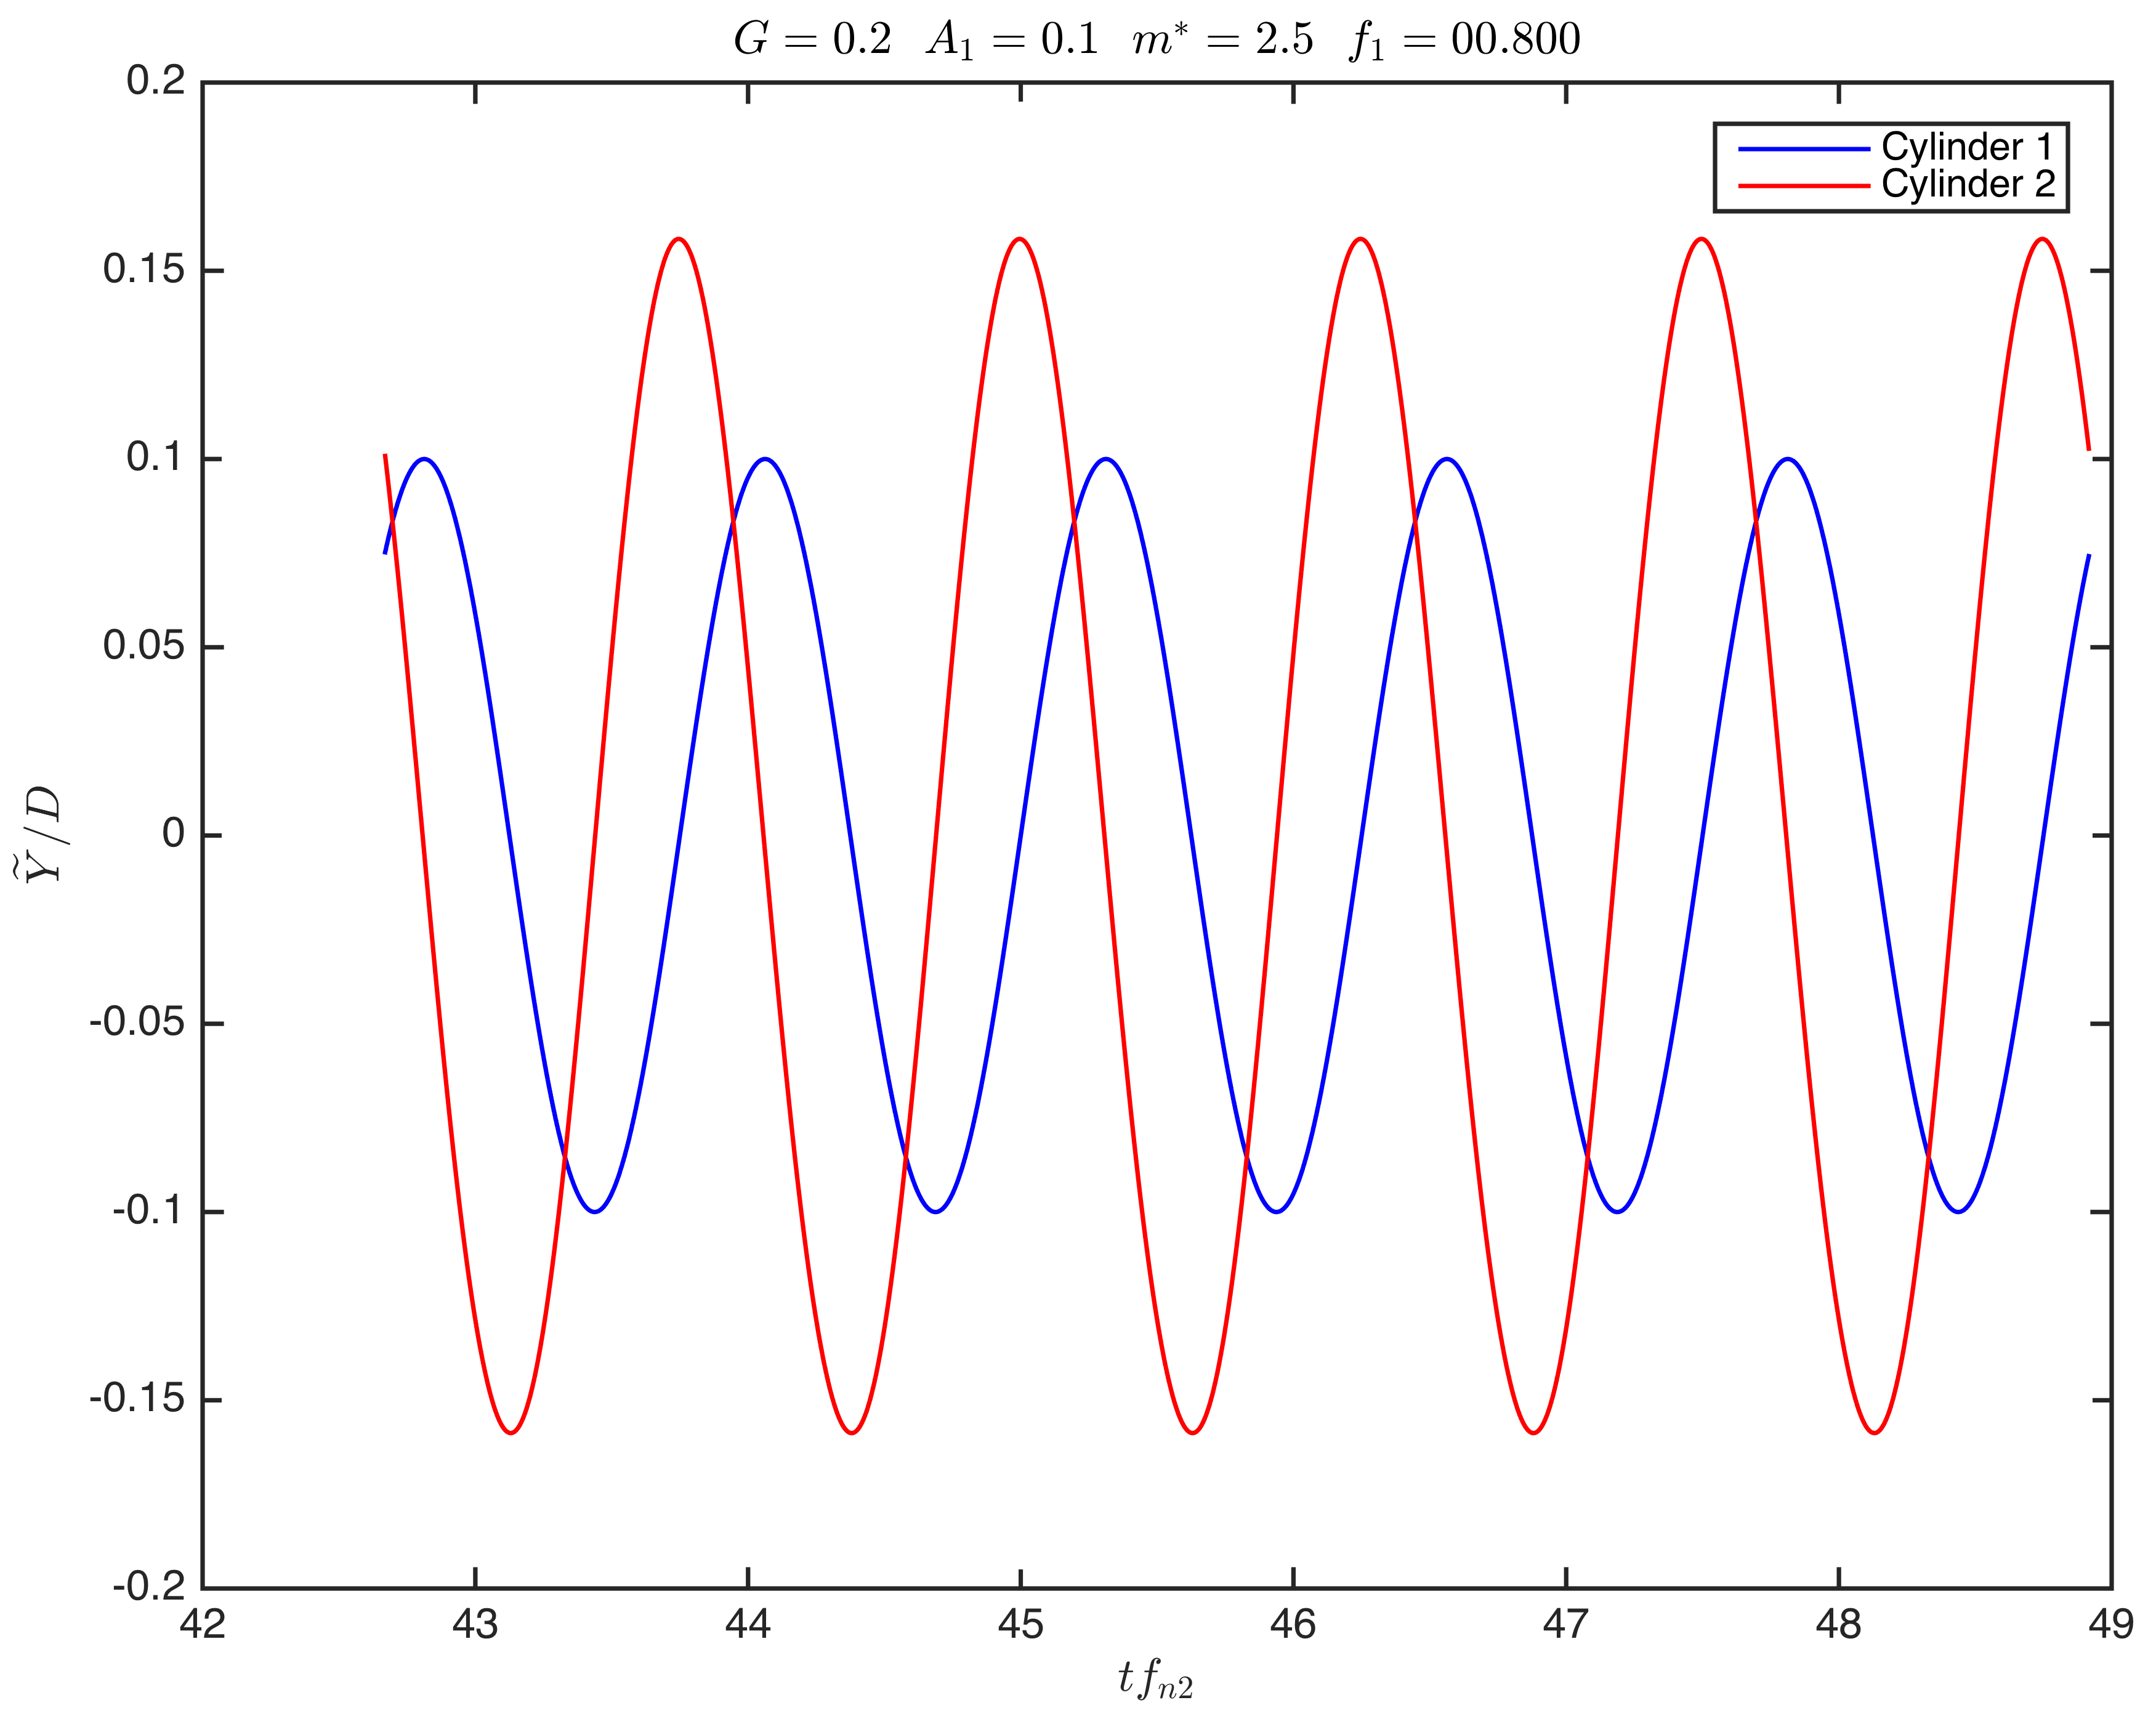
\includegraphics[width=1\linewidth]{Figs/Plotting_g0.20a0.100m2.5zl_r48_00.800_VIV02}
		\caption{$ f_1=0.8 $}
		\label{fig:freq0.8}
	\end{subfigure}\\%
	\begin{subfigure}[t]{\widthp\textwidth}
		\centering
		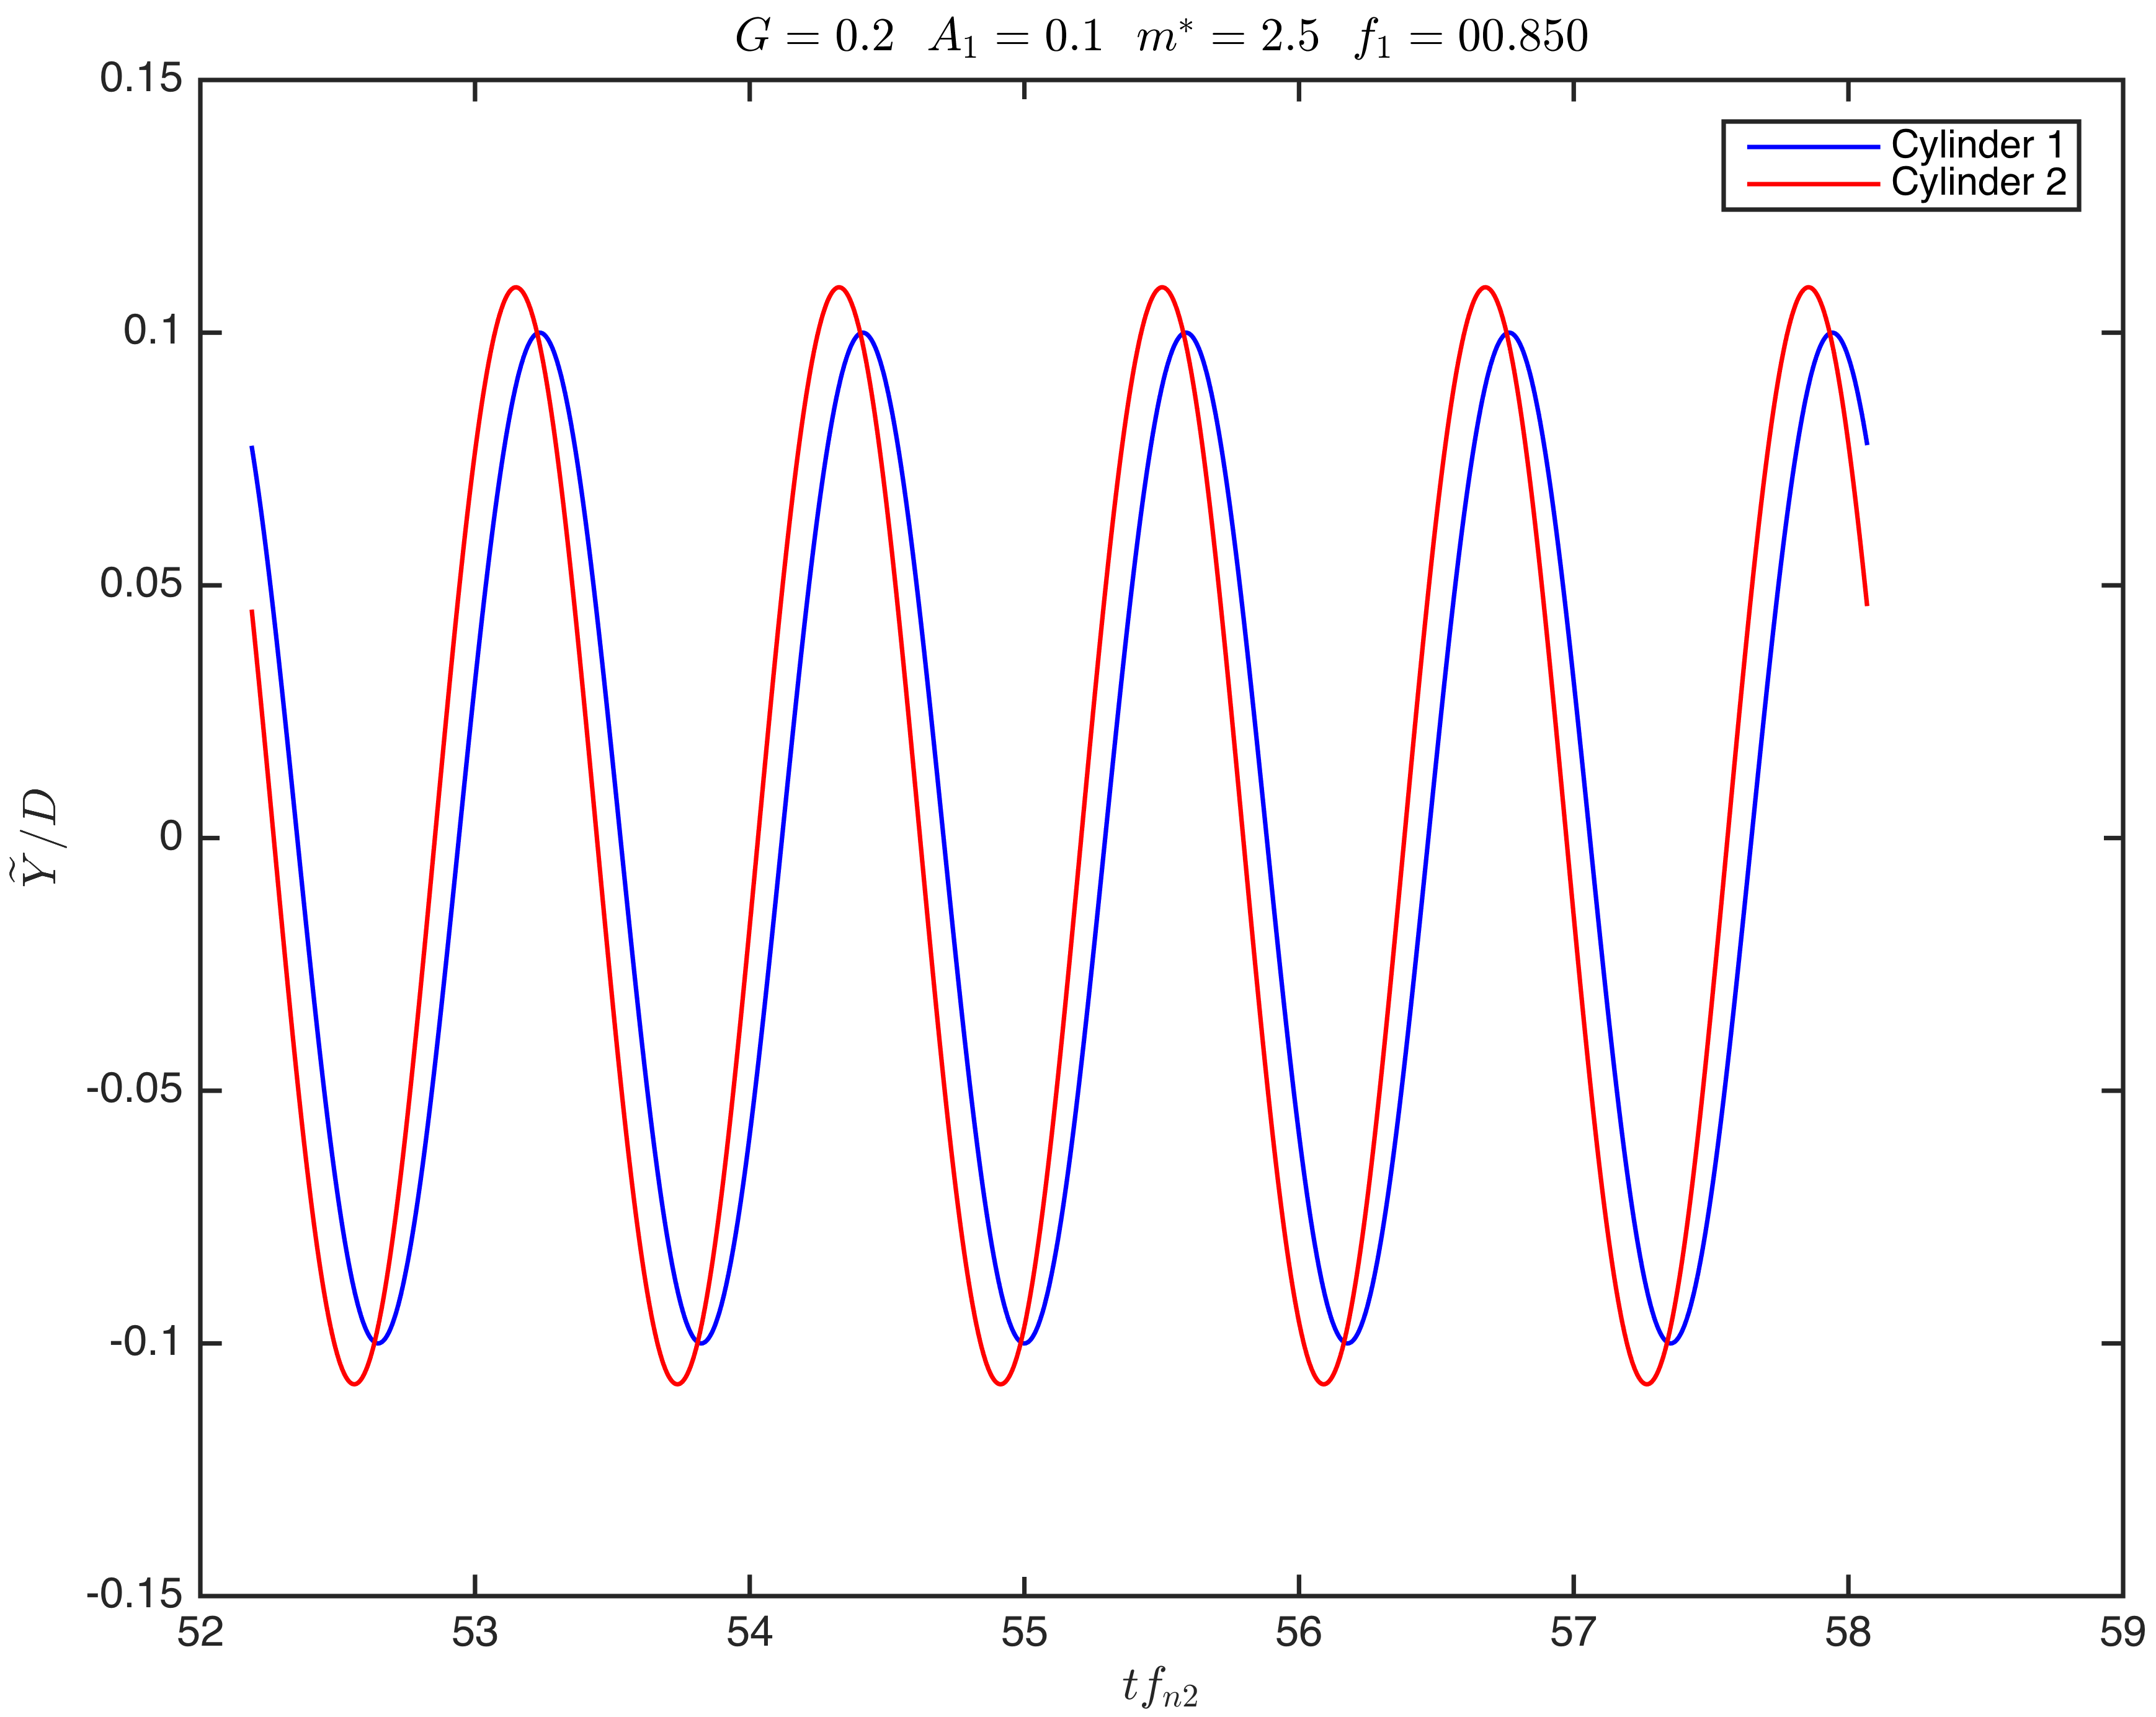
\includegraphics[width=1\linewidth]{Figs/Plotting_g0.20a0.100m2.5zl_r48_00.850_VIV02}
		\caption{$ f_1=0.85 $}
		\label{fig:freq0.85}
	\end{subfigure}%	
	\begin{subfigure}[t]{\widthp\textwidth}
		\centering
		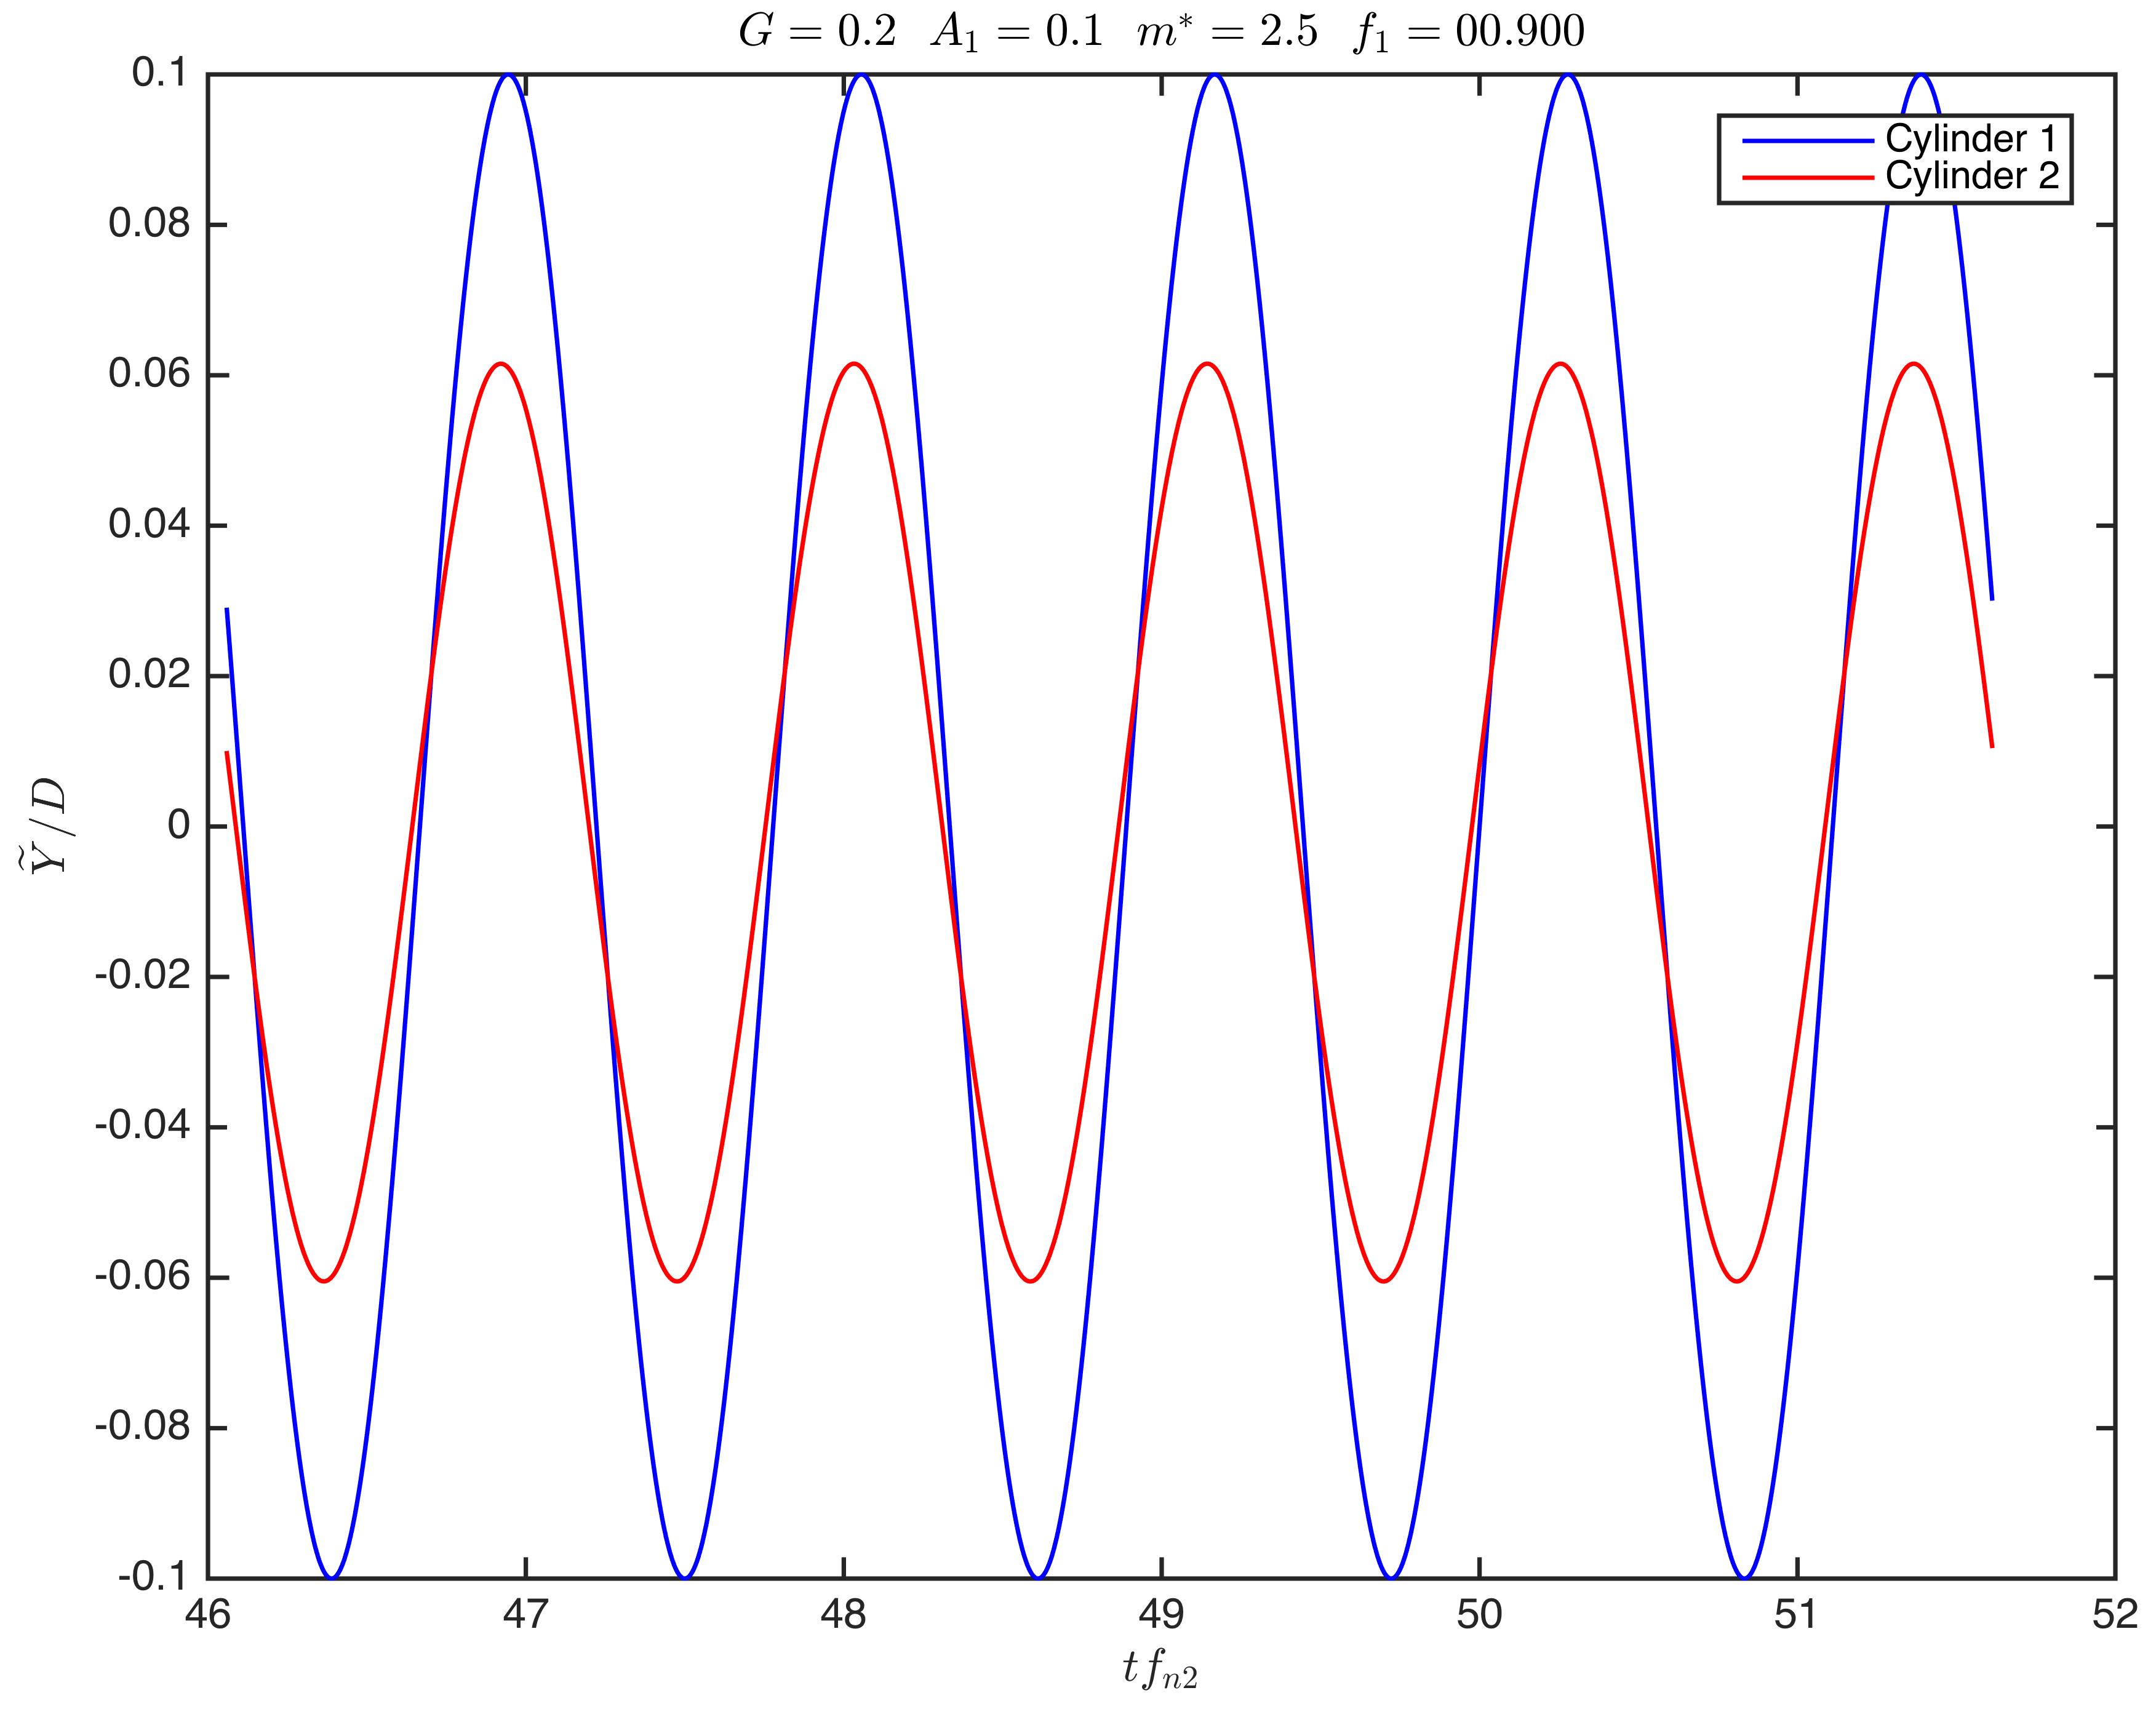
\includegraphics[width=1\linewidth]{Figs/Plotting_g0.20a0.100m2.5zl_r48_00.900_VIV02}
		\caption{$ f_1=0.9 $}
		\label{fig:freq0.9}
	\end{subfigure}\\%
	\begin{subfigure}[t]{\widthp\textwidth}
		\centering
		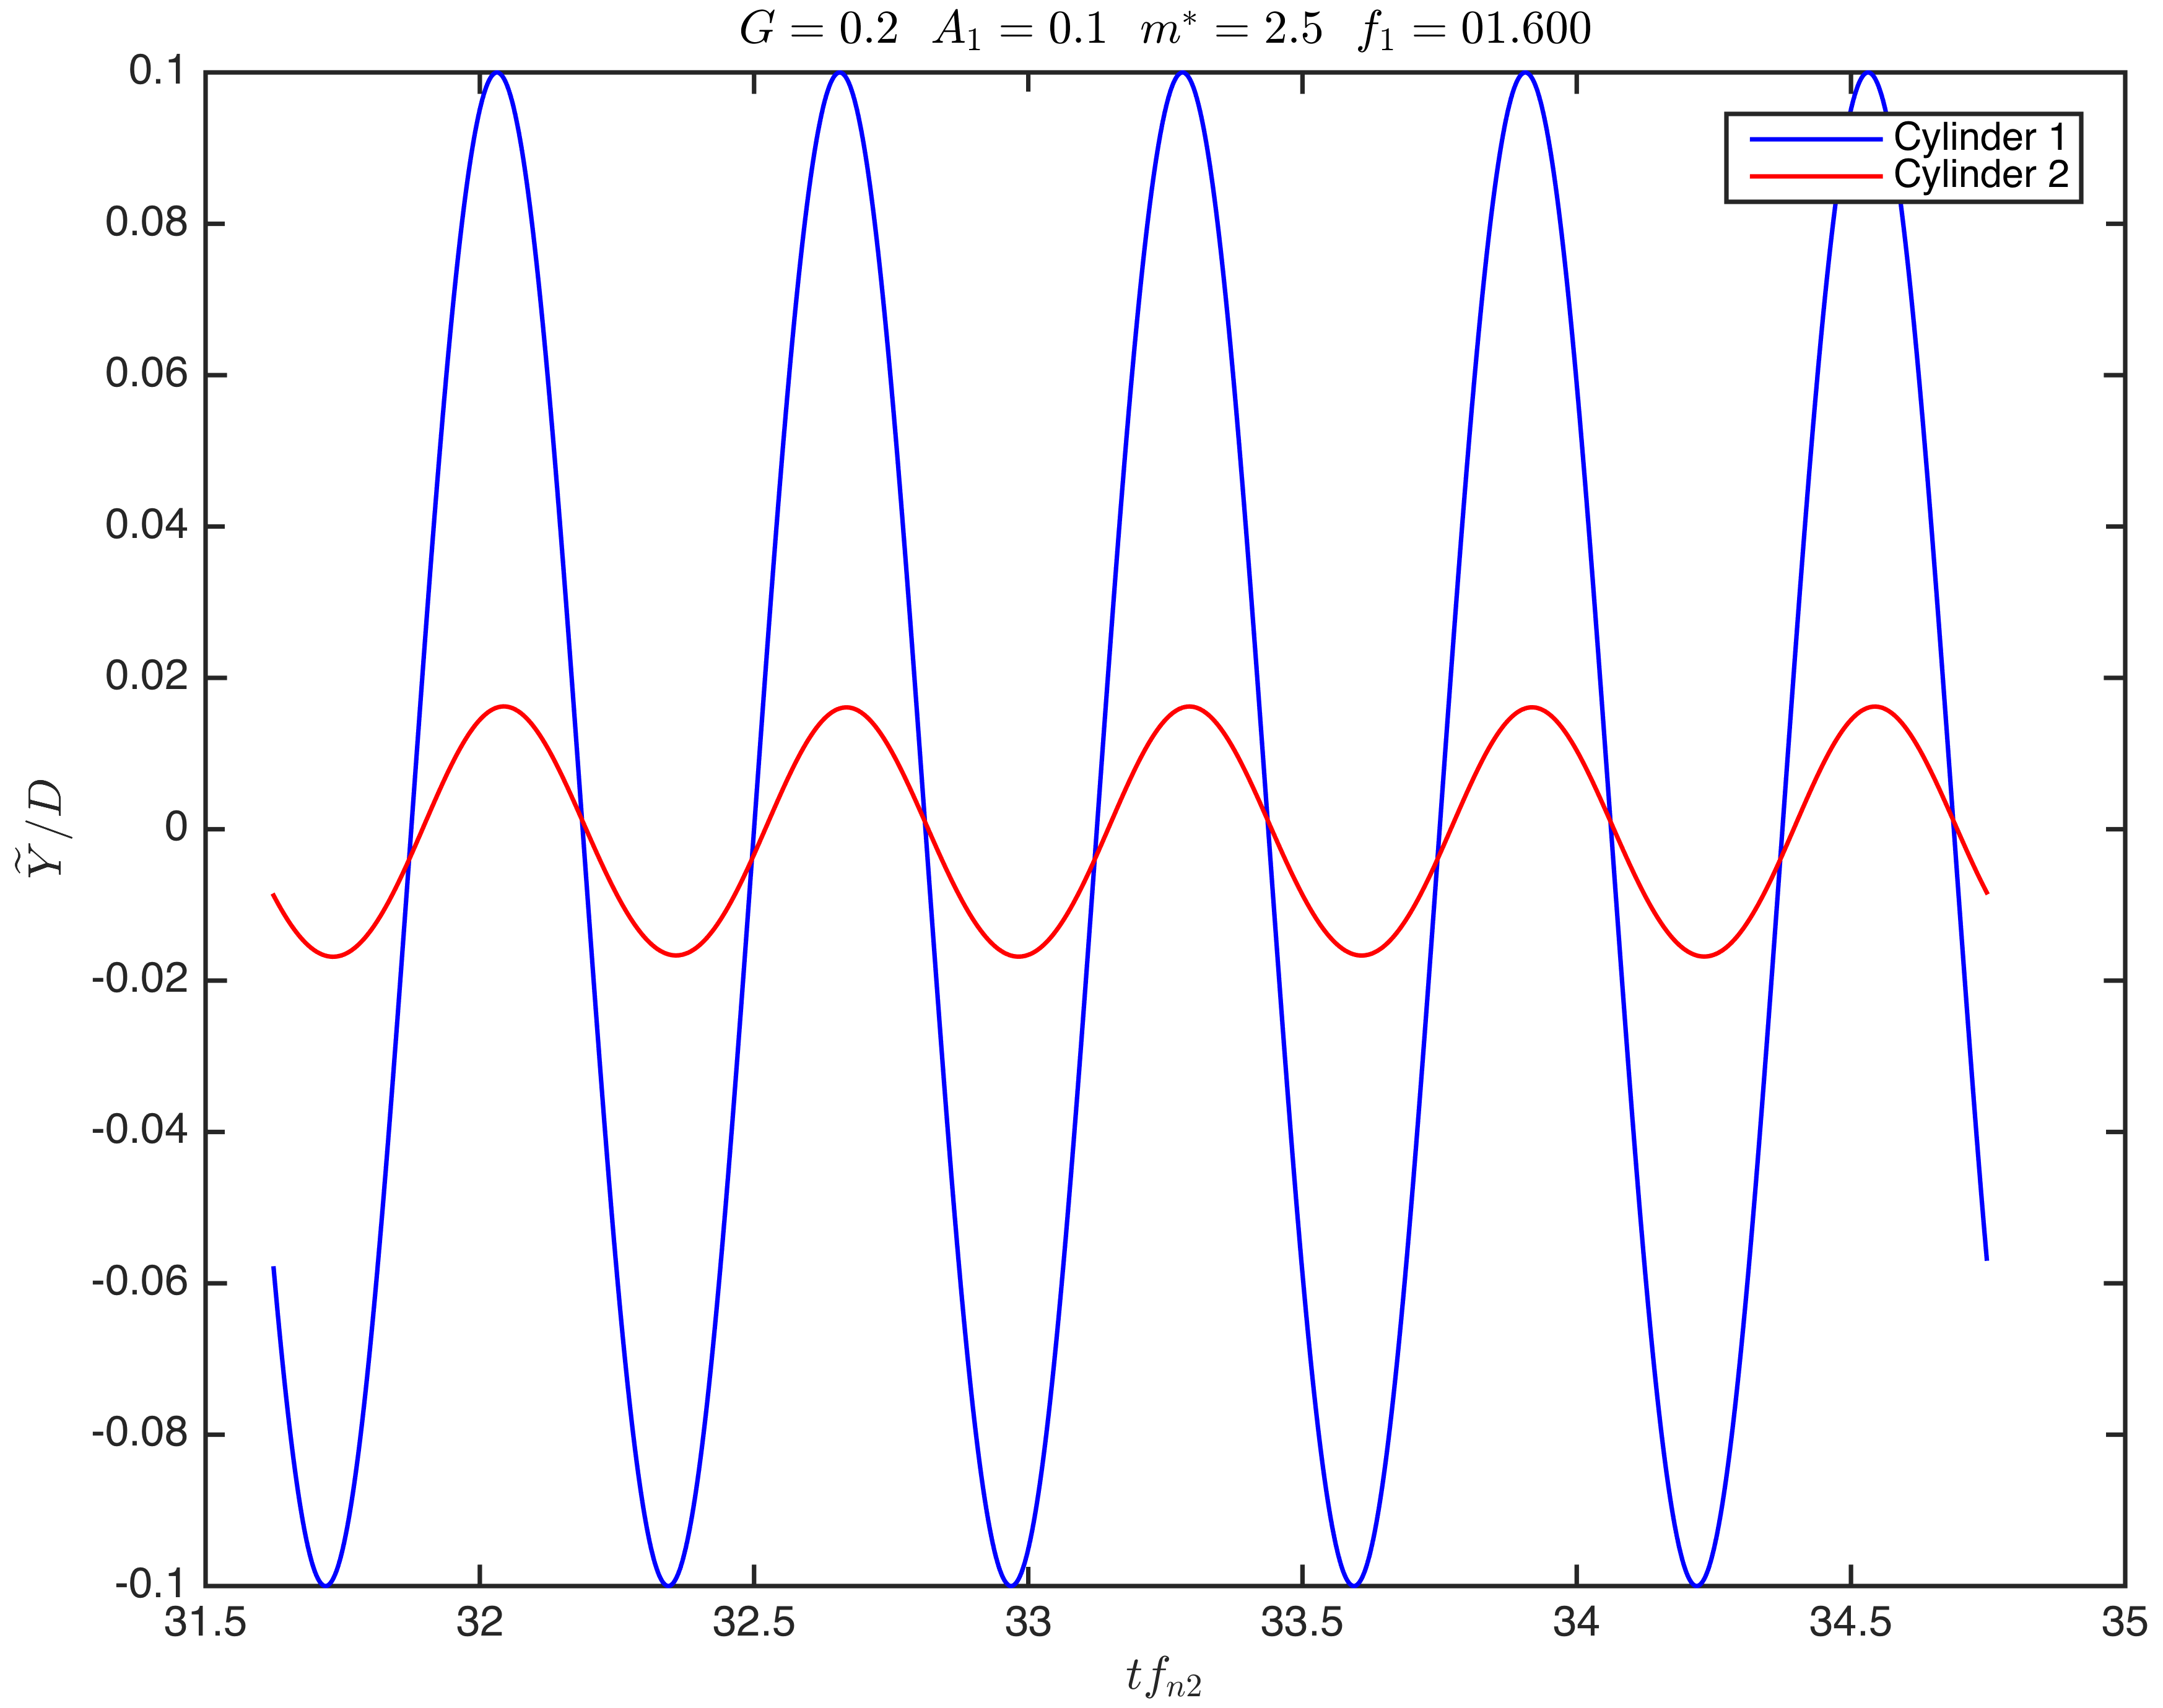
\includegraphics[width=1\linewidth]{Figs/Plotting_g0.20a0.100m2.5zl_r48_01.600_VIV02}
		\caption{$ f_1=1.6 $}
		\label{fig:freq1.6}
	\end{subfigure}%
	\begin{subfigure}[t]{\widthp\textwidth}
		\centering
		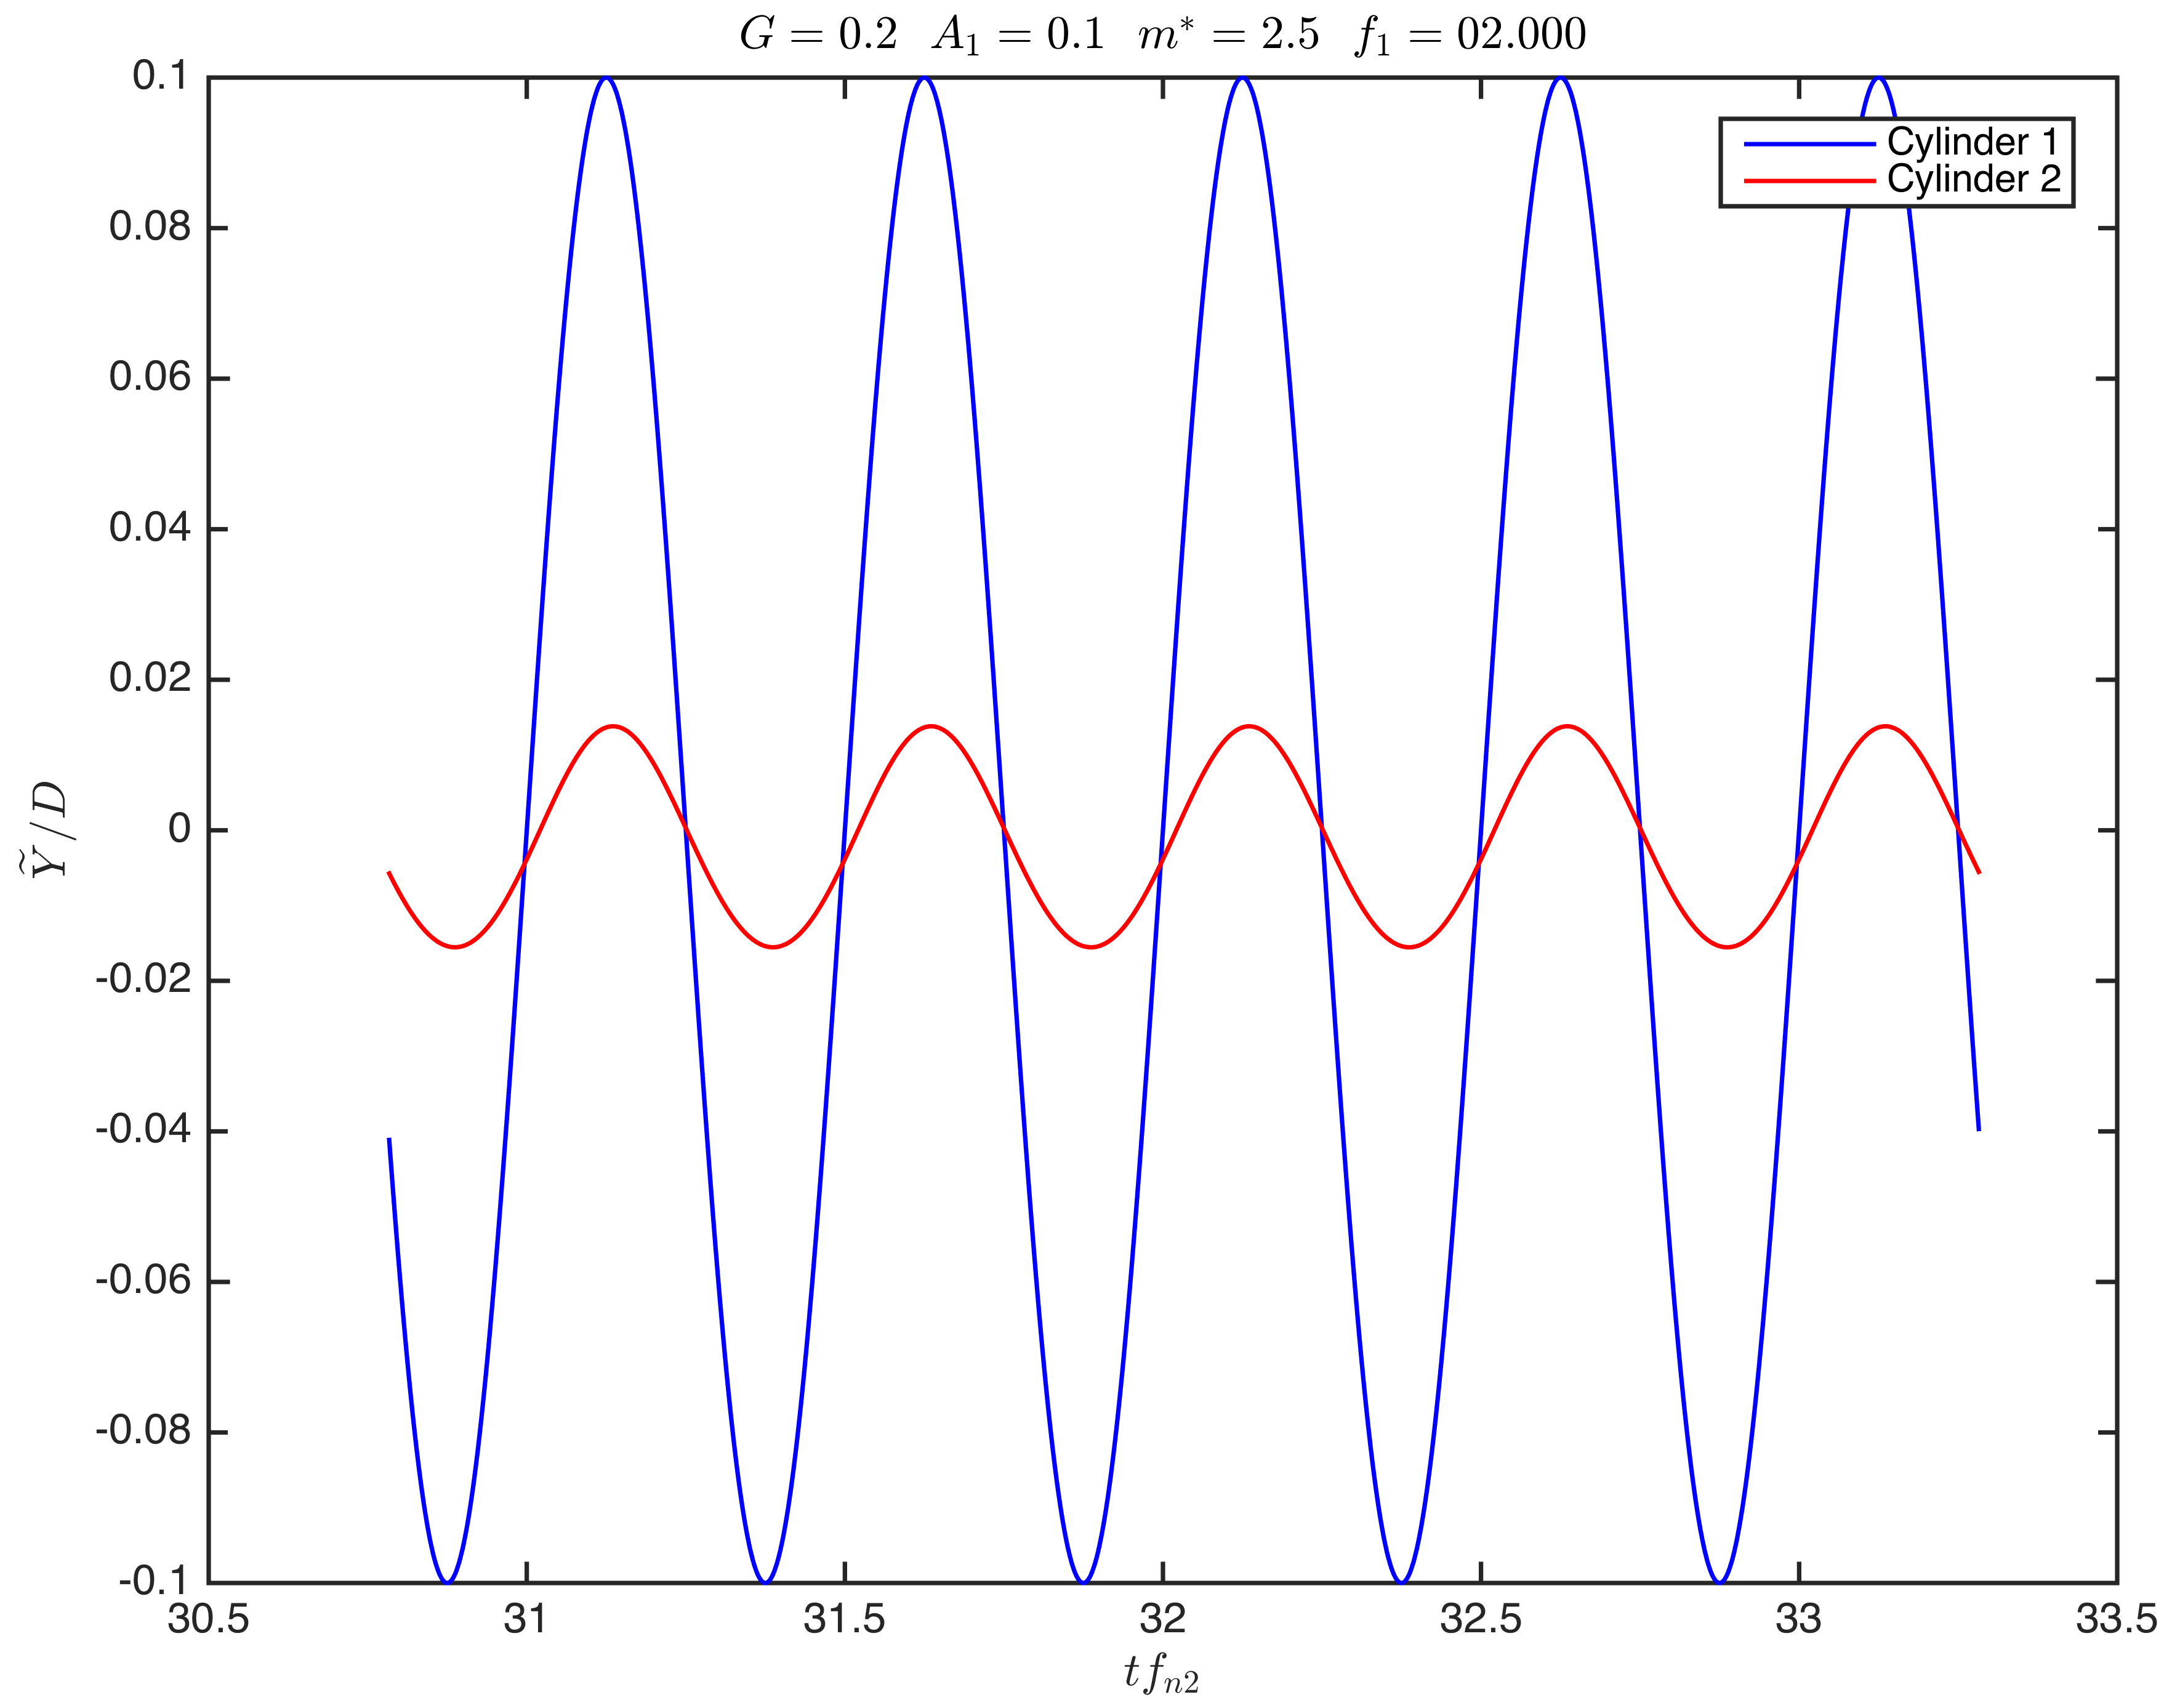
\includegraphics[width=1\linewidth]{Figs/Plotting_g0.20a0.100m2.5zl_r48_02.000_VIV02}
		\caption{$ f_1=2.0 $, in phase}
		\label{fig:freq2.0}
	\end{subfigure}\\%
	\caption{
		Comparison between Cylinder 1 and Cylinder 2's displacement histories at $ G=0.2,\ A_1=0.1,\ f_1=0.65,\ 0.8.\ 0.85,\ 0.9,\ 1.6,\ 2.0$. The blue line denotes Cylinder 1, while red line denotes Cylinder 2.
	}
	\label{fig:freqcheck}
\end{figure}

\begin{figure}[tbp]	
	\newcommand\widthp{0.5}
	\centering
	%\captionsetup{justification=centering}
	%\captionsetup[subfigure]{labelsep = none}
	%\captionsetup[subfigure]{labelformat = empty}
	\hspace*{\fill}%
	\begin{subfigure}[t]{\widthp\textwidth}
		\centering
		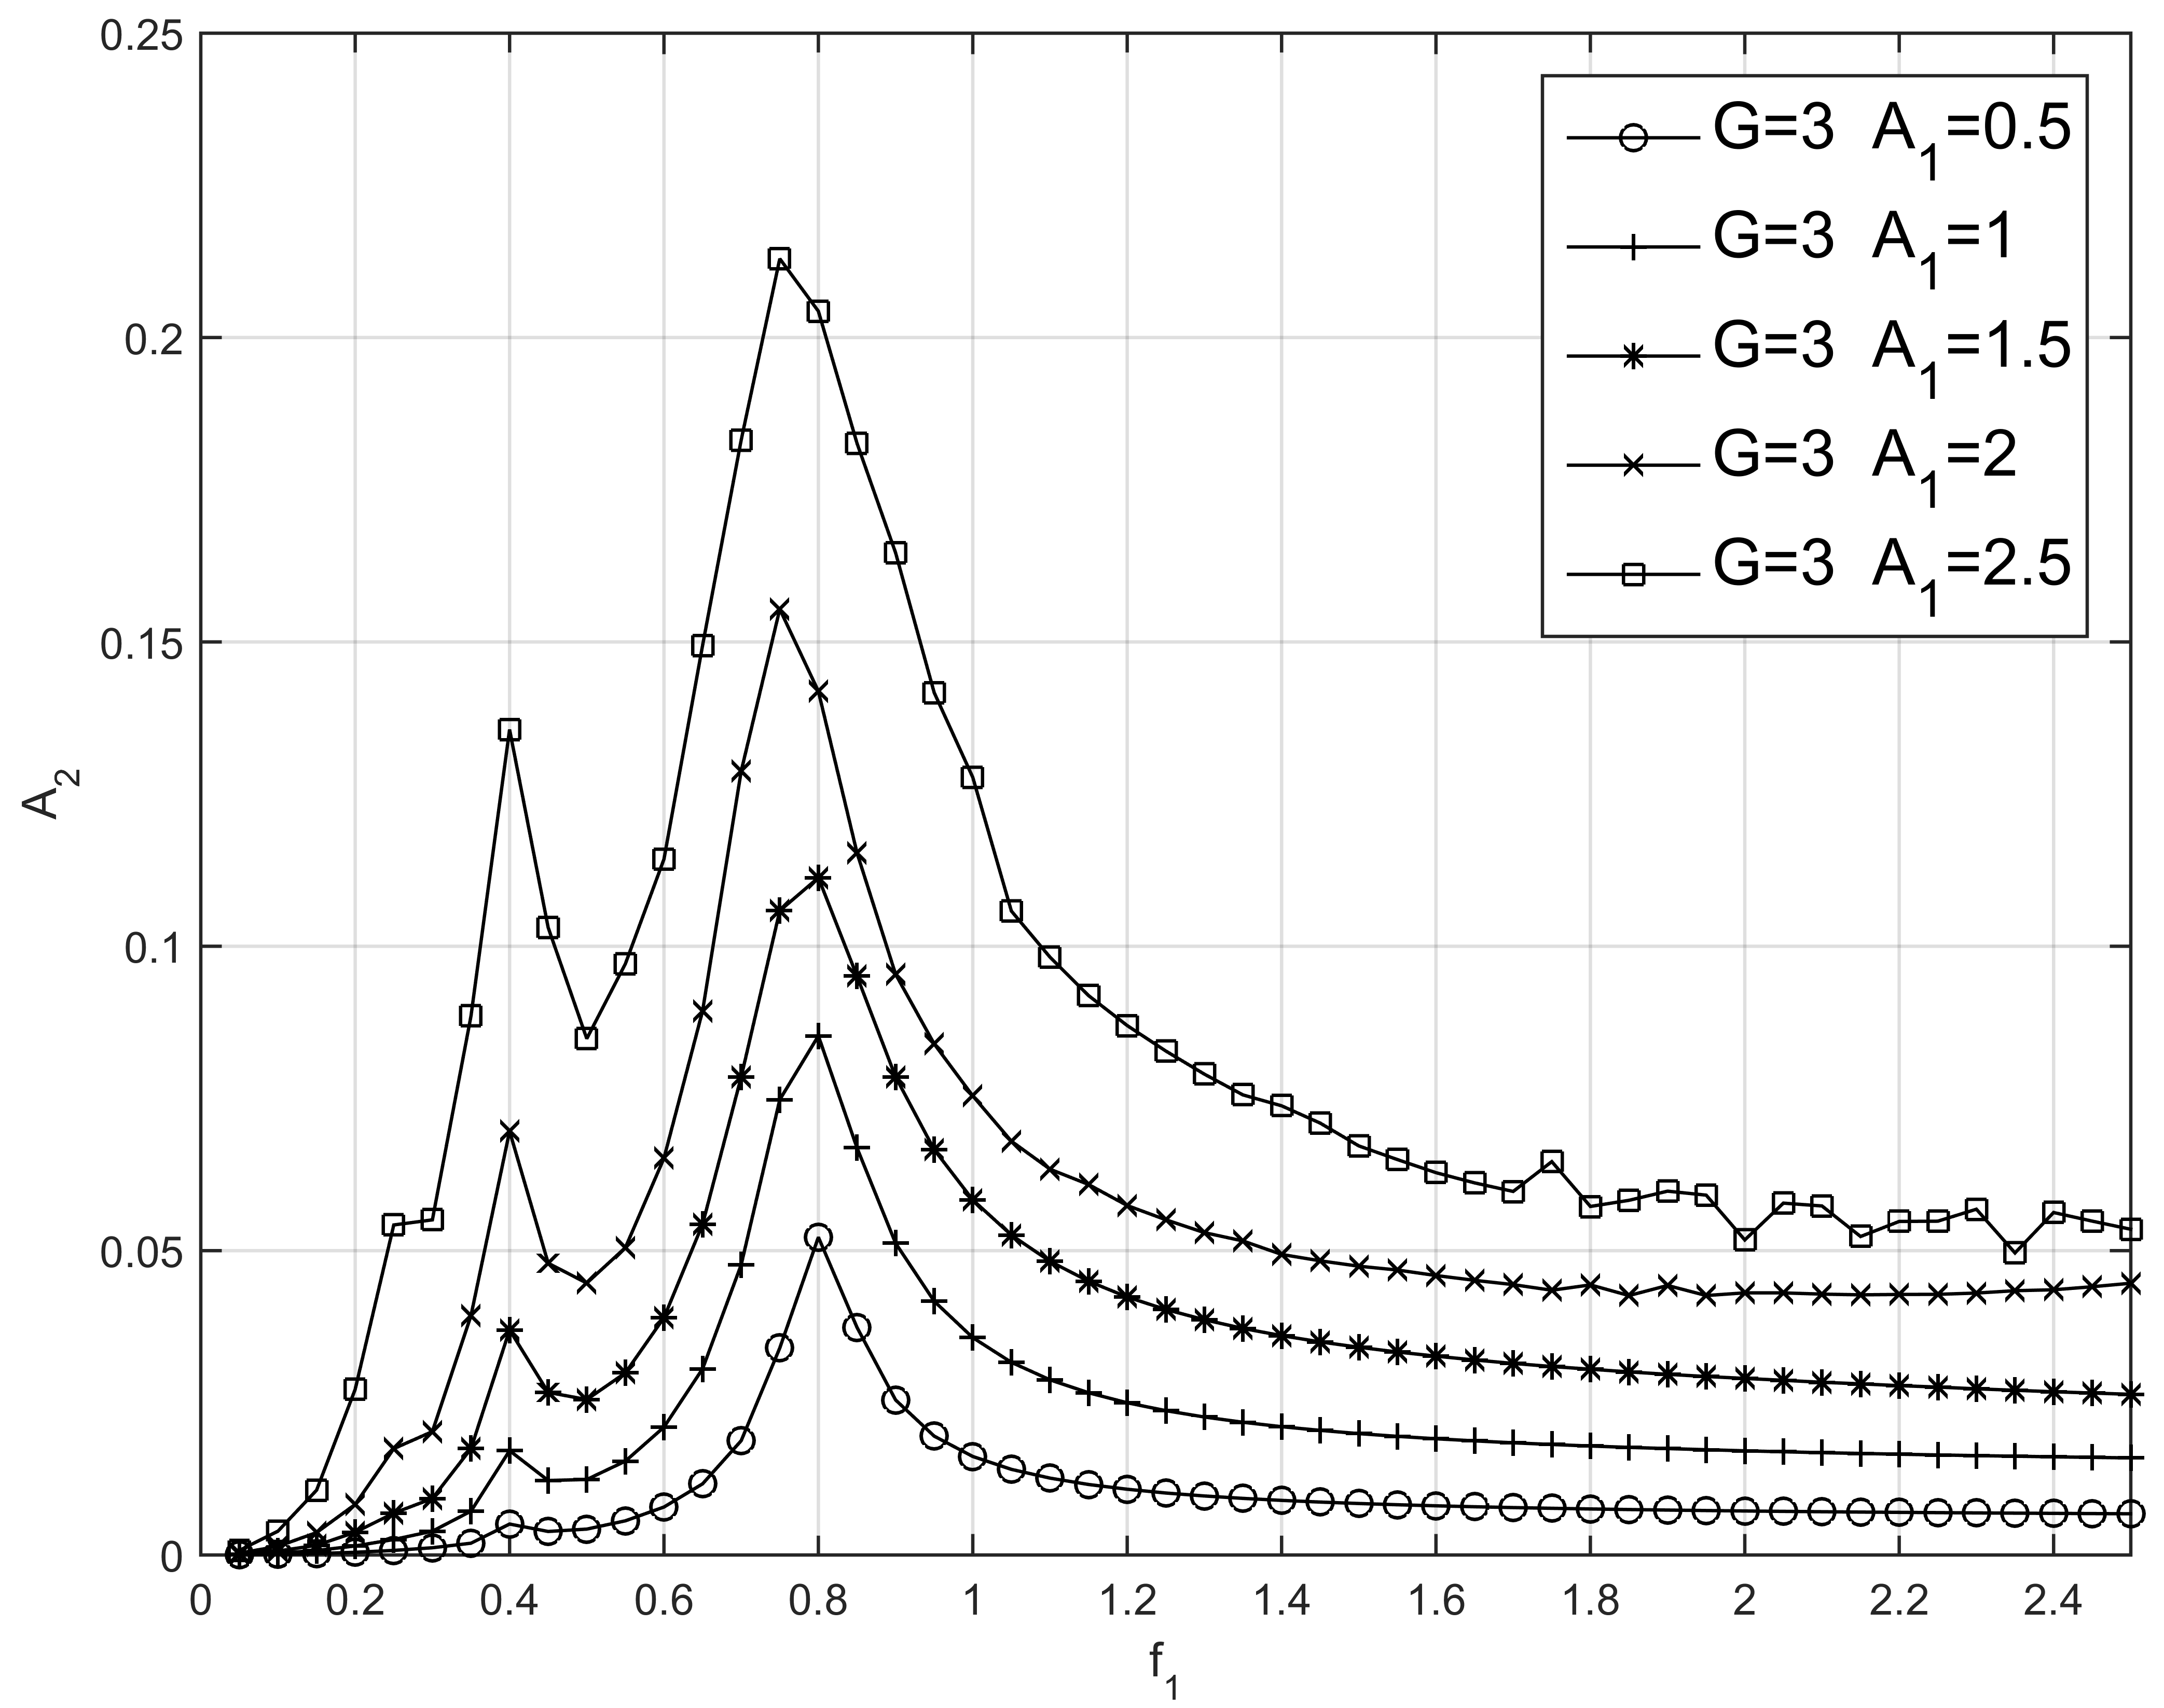
\includegraphics[width=\linewidth]{Figs/G=3_A2}
		\caption{$ G=3 $, $ f_1$-$A_2 $}
		\label{fig:g3a2}
	\end{subfigure}%
	\begin{subfigure}[t]{\widthp\textwidth}
		\centering
		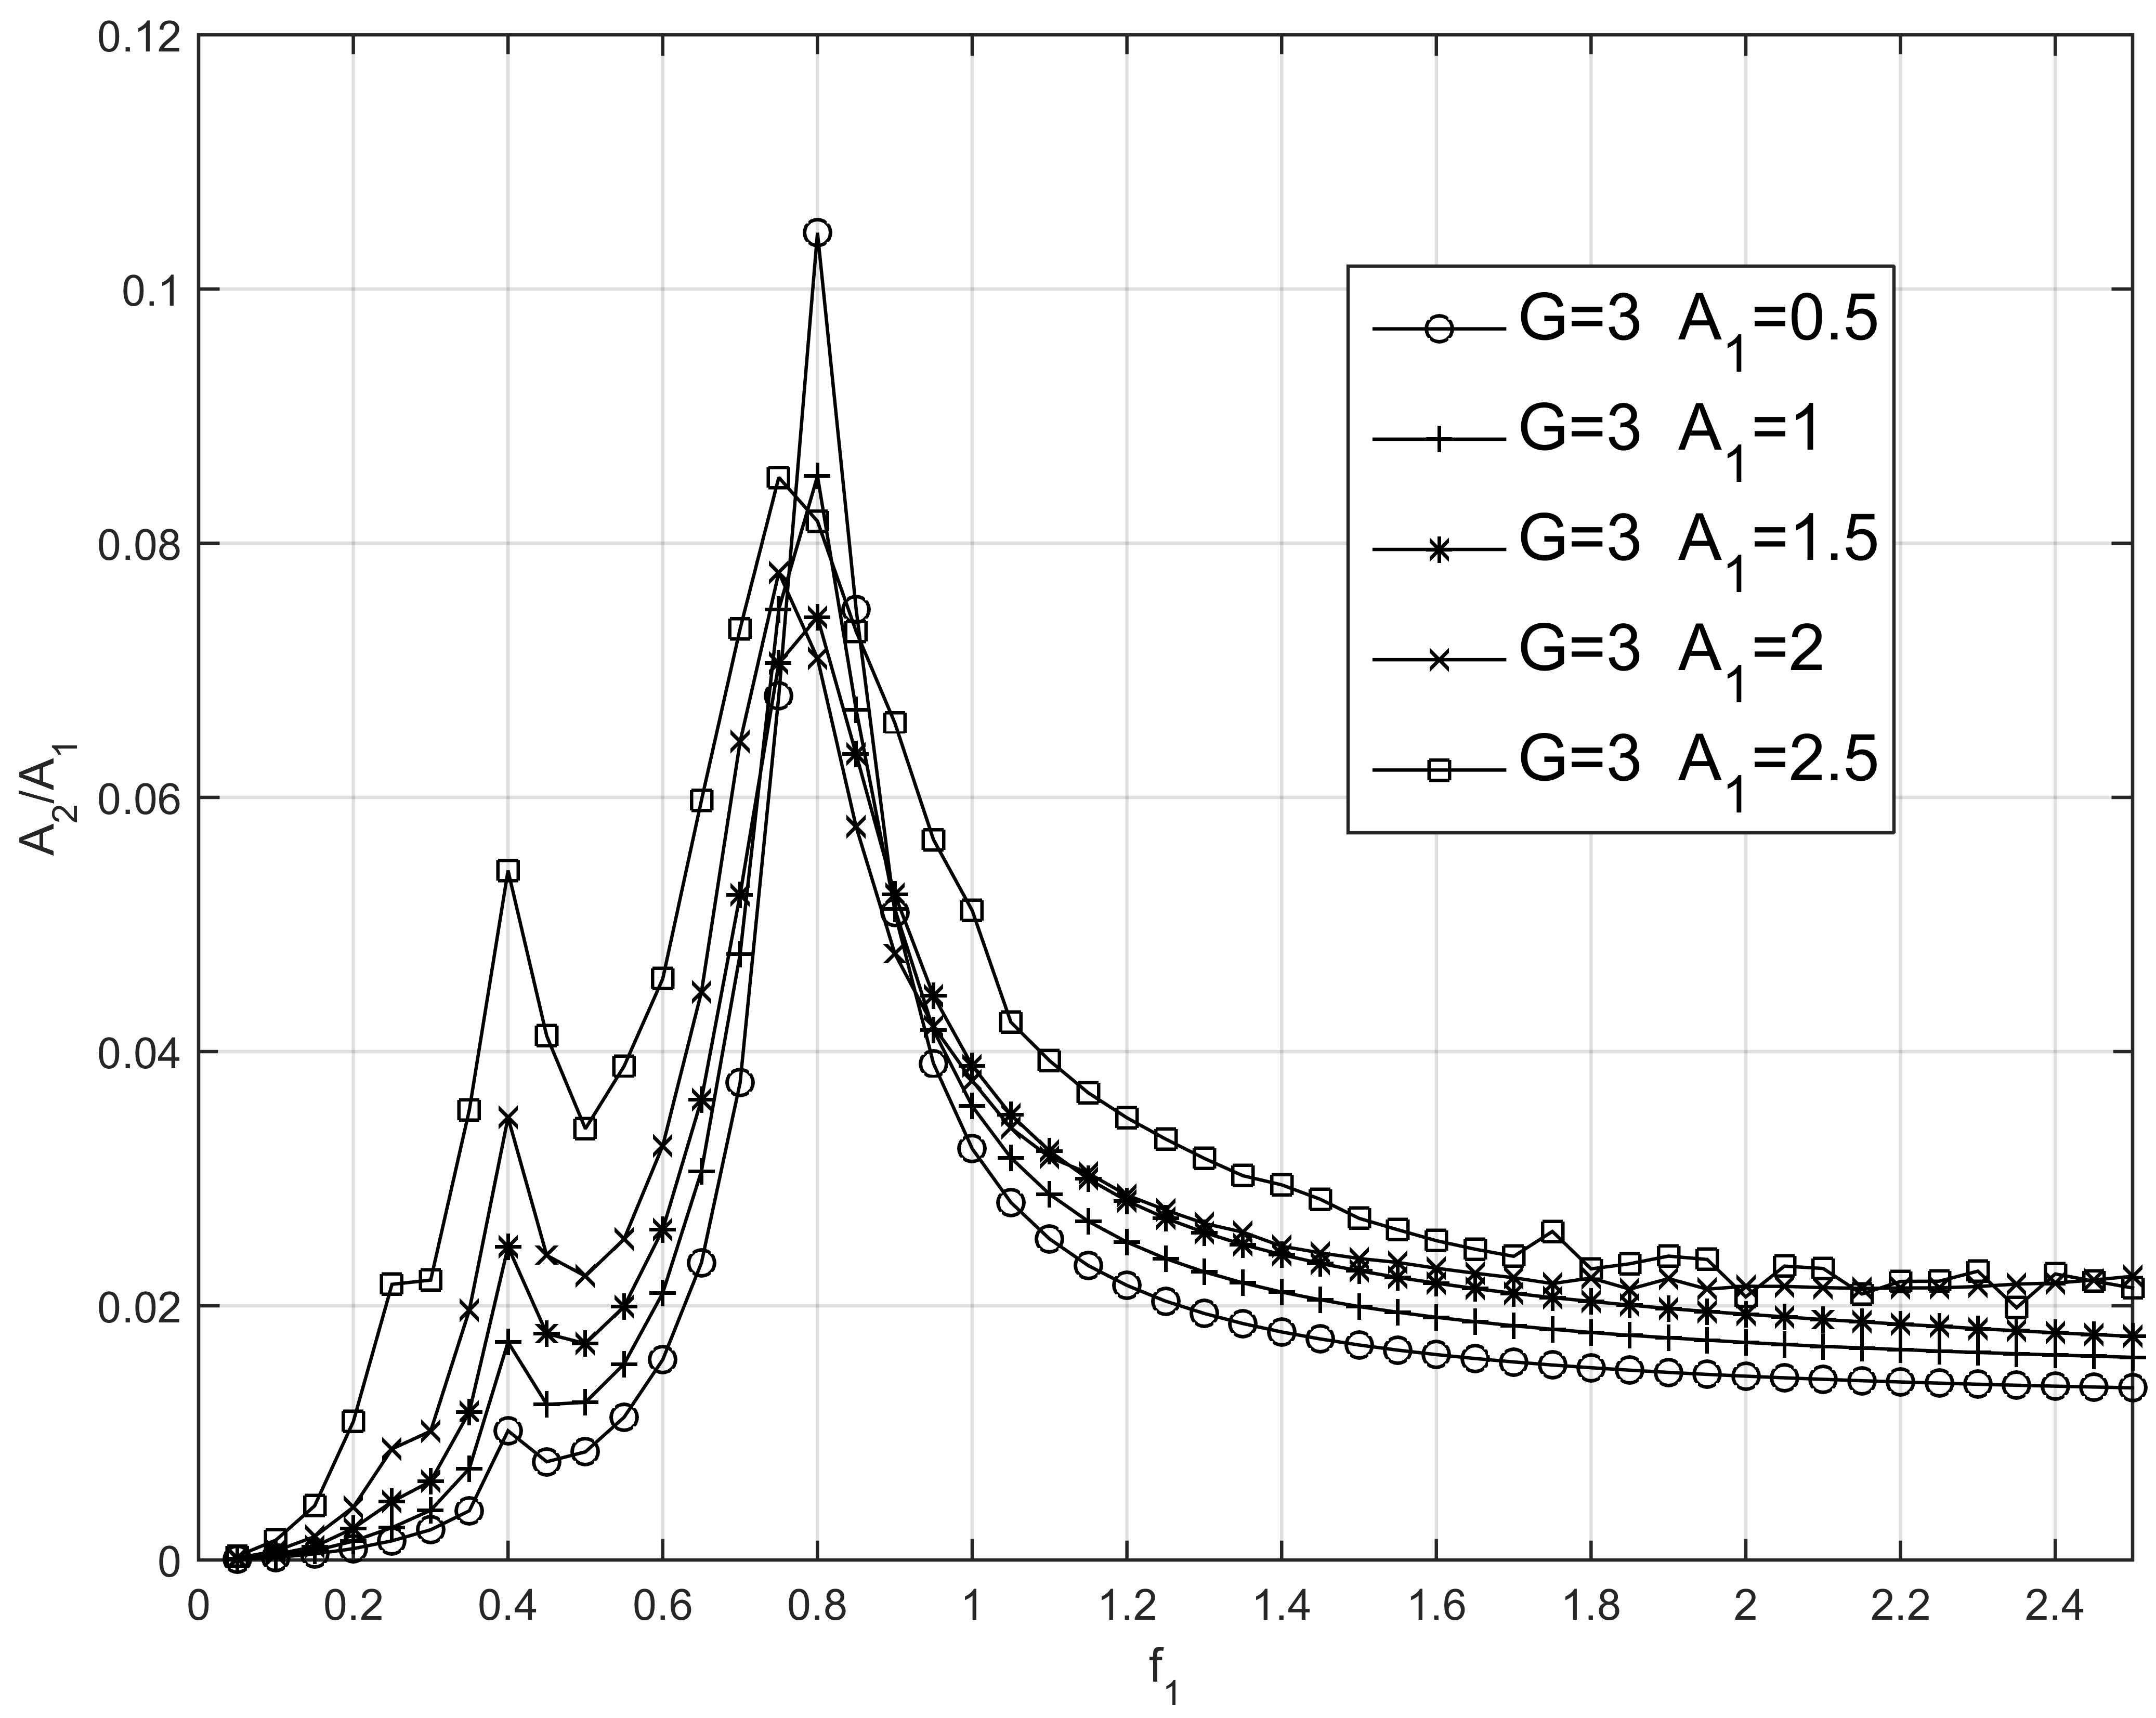
\includegraphics[width=\linewidth]{Figs/G=3_A2dA1}
		\caption{$ G=3 $, $ f_1$-$(A_2/A_1)$}
		\label{fig:g3a2da1}
	\end{subfigure}%
	\caption{
		(a) Variation of C2's response amplitude with the frequency of C1 for $ G=3, A_1=0.5,\ 1.0,\ 1.5,\ 2.0,\ 2.5 $, and (b) Variation of C2's amplification factor with the frequency of C1, for $ G=3,\ A_1=0.5,\ 1.0,\ 1.5,\ 2.0,\ 2.5 $.
	}
	\label{fig:g3}
\end{figure}

\Cref{fig:g3a2} shows the relationship between C2's response amplitude ($ A_2 $) and the C1's frequency $ f_1 $. Generally speaking, C2's response amplitude in \Cref{fig:g3a2} ranges from almost 0 to 0.22. There are two peaks: a smaller one at $ 0.4f_n $ and a greater one at $ 0.8f_n $. For the same $ f_1 $, cases with greater $ A_1 $ always have greater $ A_2 $. As $ f_1 $ increases beyond 1.6, $ A_2 $ does not change significantly.

\Cref{fig:g3a2da1} demonstrates the amplification of the vibration, with the y-axis representing $A_{2}/A_{1}$. For the peak at $f_{n} = 0.4$, the pattern is similar to \Cref{fig:g3a2}. However, the major peak at $f_{n} = 0.8$ has a pattern that is different from \Cref{fig:g3a2}. The case with $A_{1} = 0.5$ has the largest value of $A_{2}/A_{1}$ being 0.104; the cases with $A_{1}= 1\ \&\ 2.5$ have the peak value of $A_{2}/A_{1}$ being 0.085; when $A_{1} = 1.5$ and 2.0, the peak $A_{2}/A_{1}$ are 0.078 and 0.075, respectively. The rise of $A_{1}$ causes the decrease of $(A_{2}/A_{1})_{peak}$ until $A_{1} = 1.5$, after which the change in $(A_{2}/A_{1})_{peak}$ is small. 

\Cref{fig:A2dA1} demonstrates the variation of $ A_2/A_1 $ with $ f_1 $ when $ G =0.2$, 1.0, 1.25 and $ A_1 =0.025 \sim 1$. On the whole, for the cases simulated, C2's relative response amplitude $ A_2/A_1 $ in \Cref{fig:A2dA1} varies from 0 to 2. Similar to \Cref{fig:g3a2da1}, there is one large peak around $ f_1 =0.8$ accompanied by a small peak at $ f_1 =0.4$. The values of $ A_2/A_1 $ for $ G =0.2 $ are generally larger than those for $ G =1,\ 1.25$, and the patterns of lines for $ G =0.2$, 1 and 1.25 are very similar. For $ G =0.2$, 1 and 1.25, $ A_1 $ and $ (A_2/A_1)_{peak} $ are inversely related. Moreover, $ A_1 $ is also inversely related to the resonance frequency, i.e.\ the $ f_1 $ corresponding to $ (A_2/A_1)_{peak} $. As $ f_1 $ increases above 1.0, $ A_2/A_1 $ gradually drops.


\begin{figure}[p]	
	\newcommand\widthp{0.5}
	\centering
	%\captionsetup{justification=centering}
	%\captionsetup[subfigure]{labelsep = none}
	%\captionsetup[subfigure]{labelformat = empty}
	\hspace*{\fill}%
	\begin{subfigure}[t]{\widthp\textwidth}
		\centering
		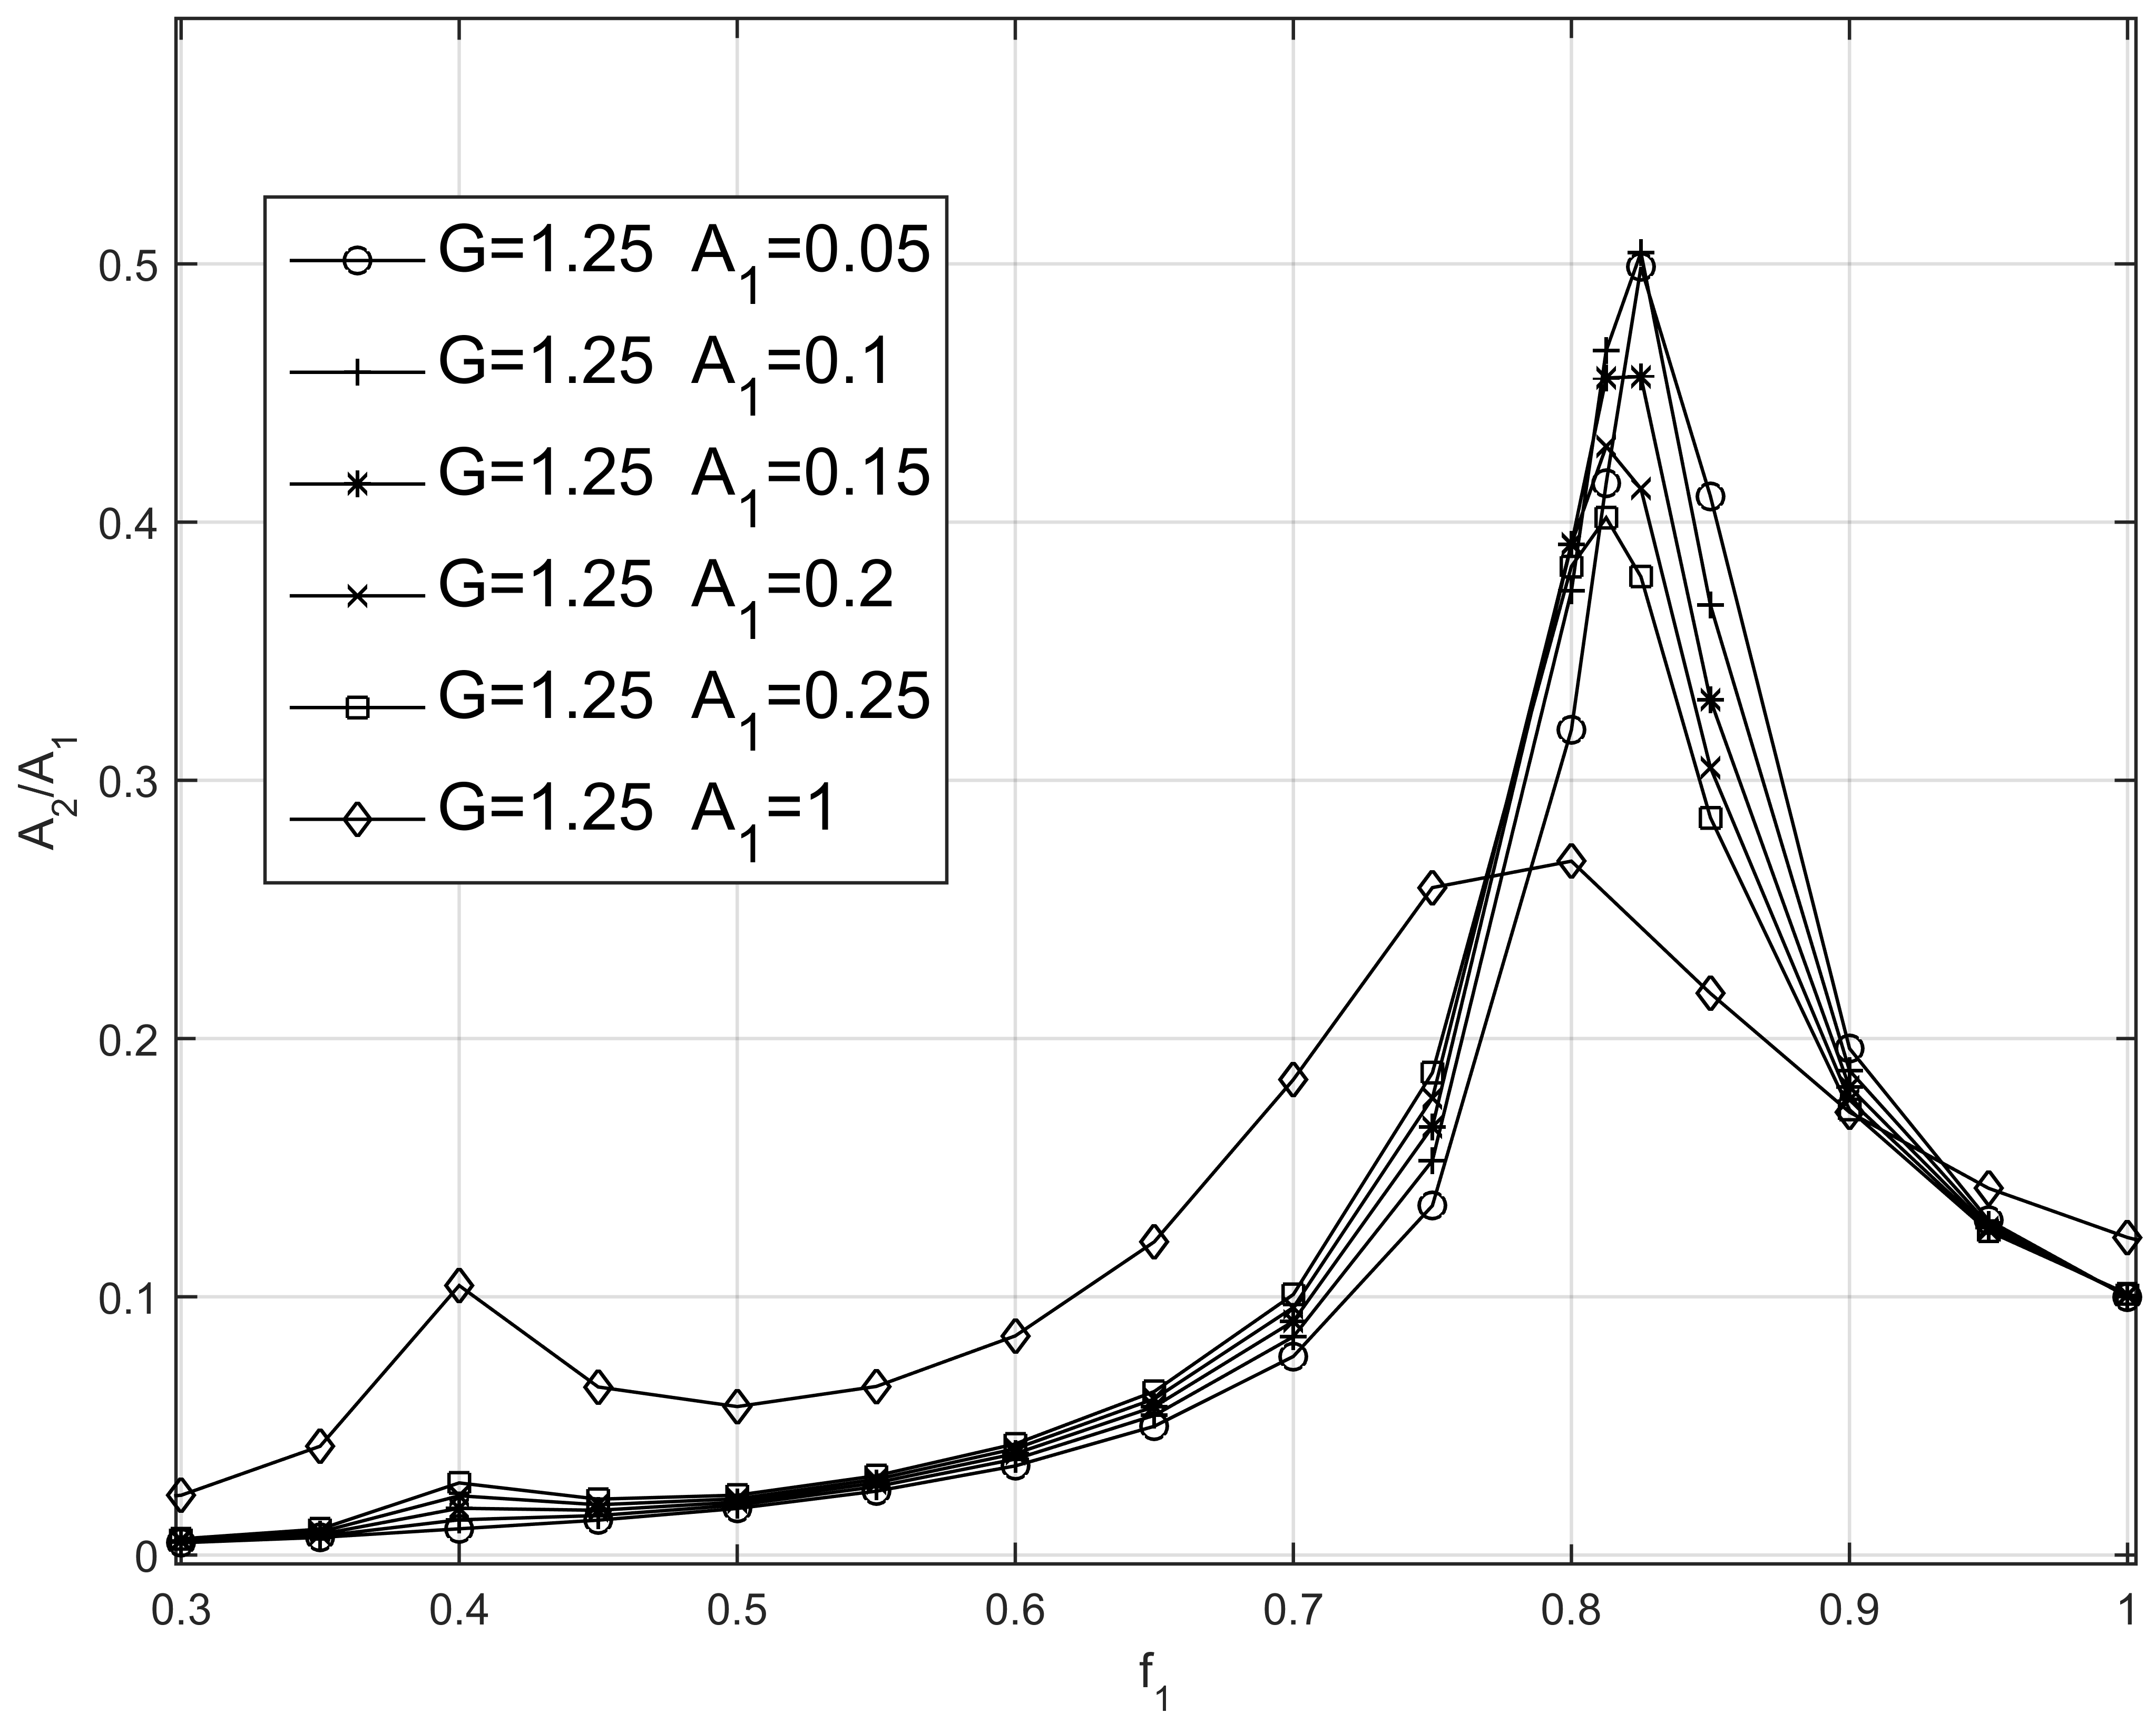
\includegraphics[width=\linewidth]{Figs/G=1.25_A2dA1.png}
		\caption{$ G=1.25 $, overview}
		\label{fig:g125a2da1}
	\end{subfigure}%
	\begin{subfigure}[t]{\widthp\textwidth}
		\centering
		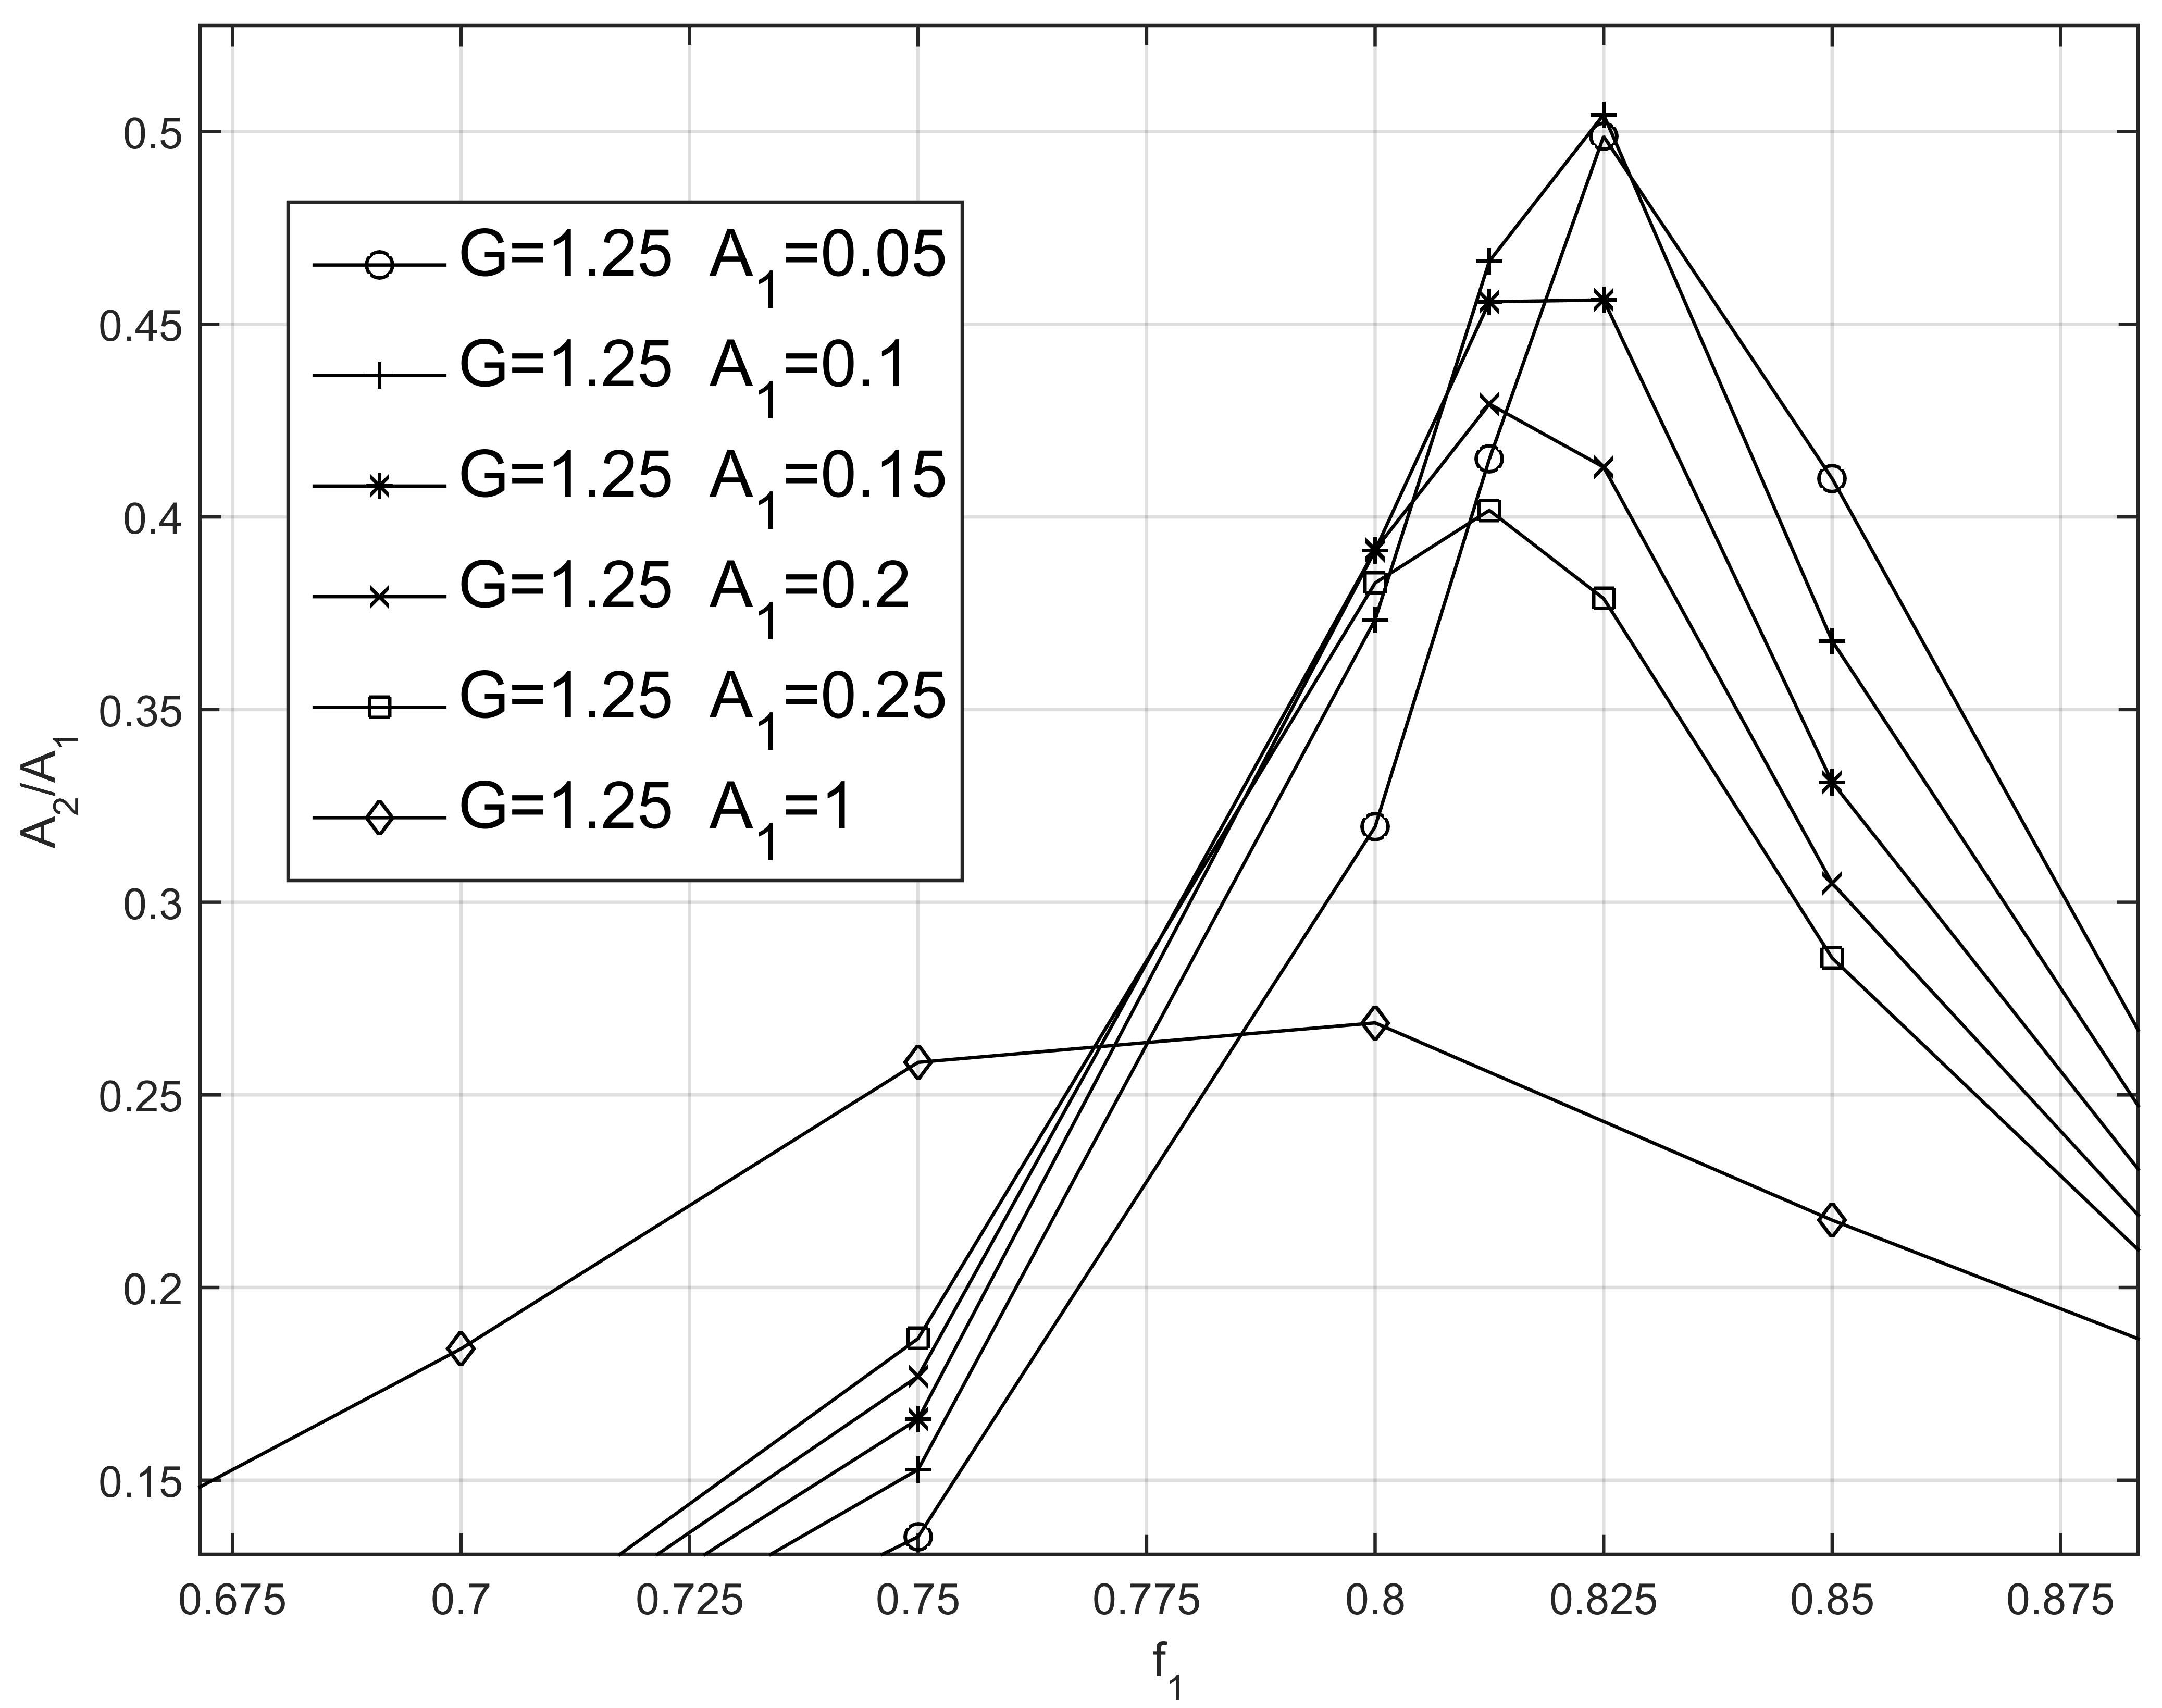
\includegraphics[width=\linewidth]{Figs/G=1.25_A2dA1_details.png}
		\caption{$ G=1.25 $, close-up}
		\label{fig:g125a2da1details}
	\end{subfigure}\\%	
	\begin{subfigure}[t]{\widthp\textwidth}
		\centering
		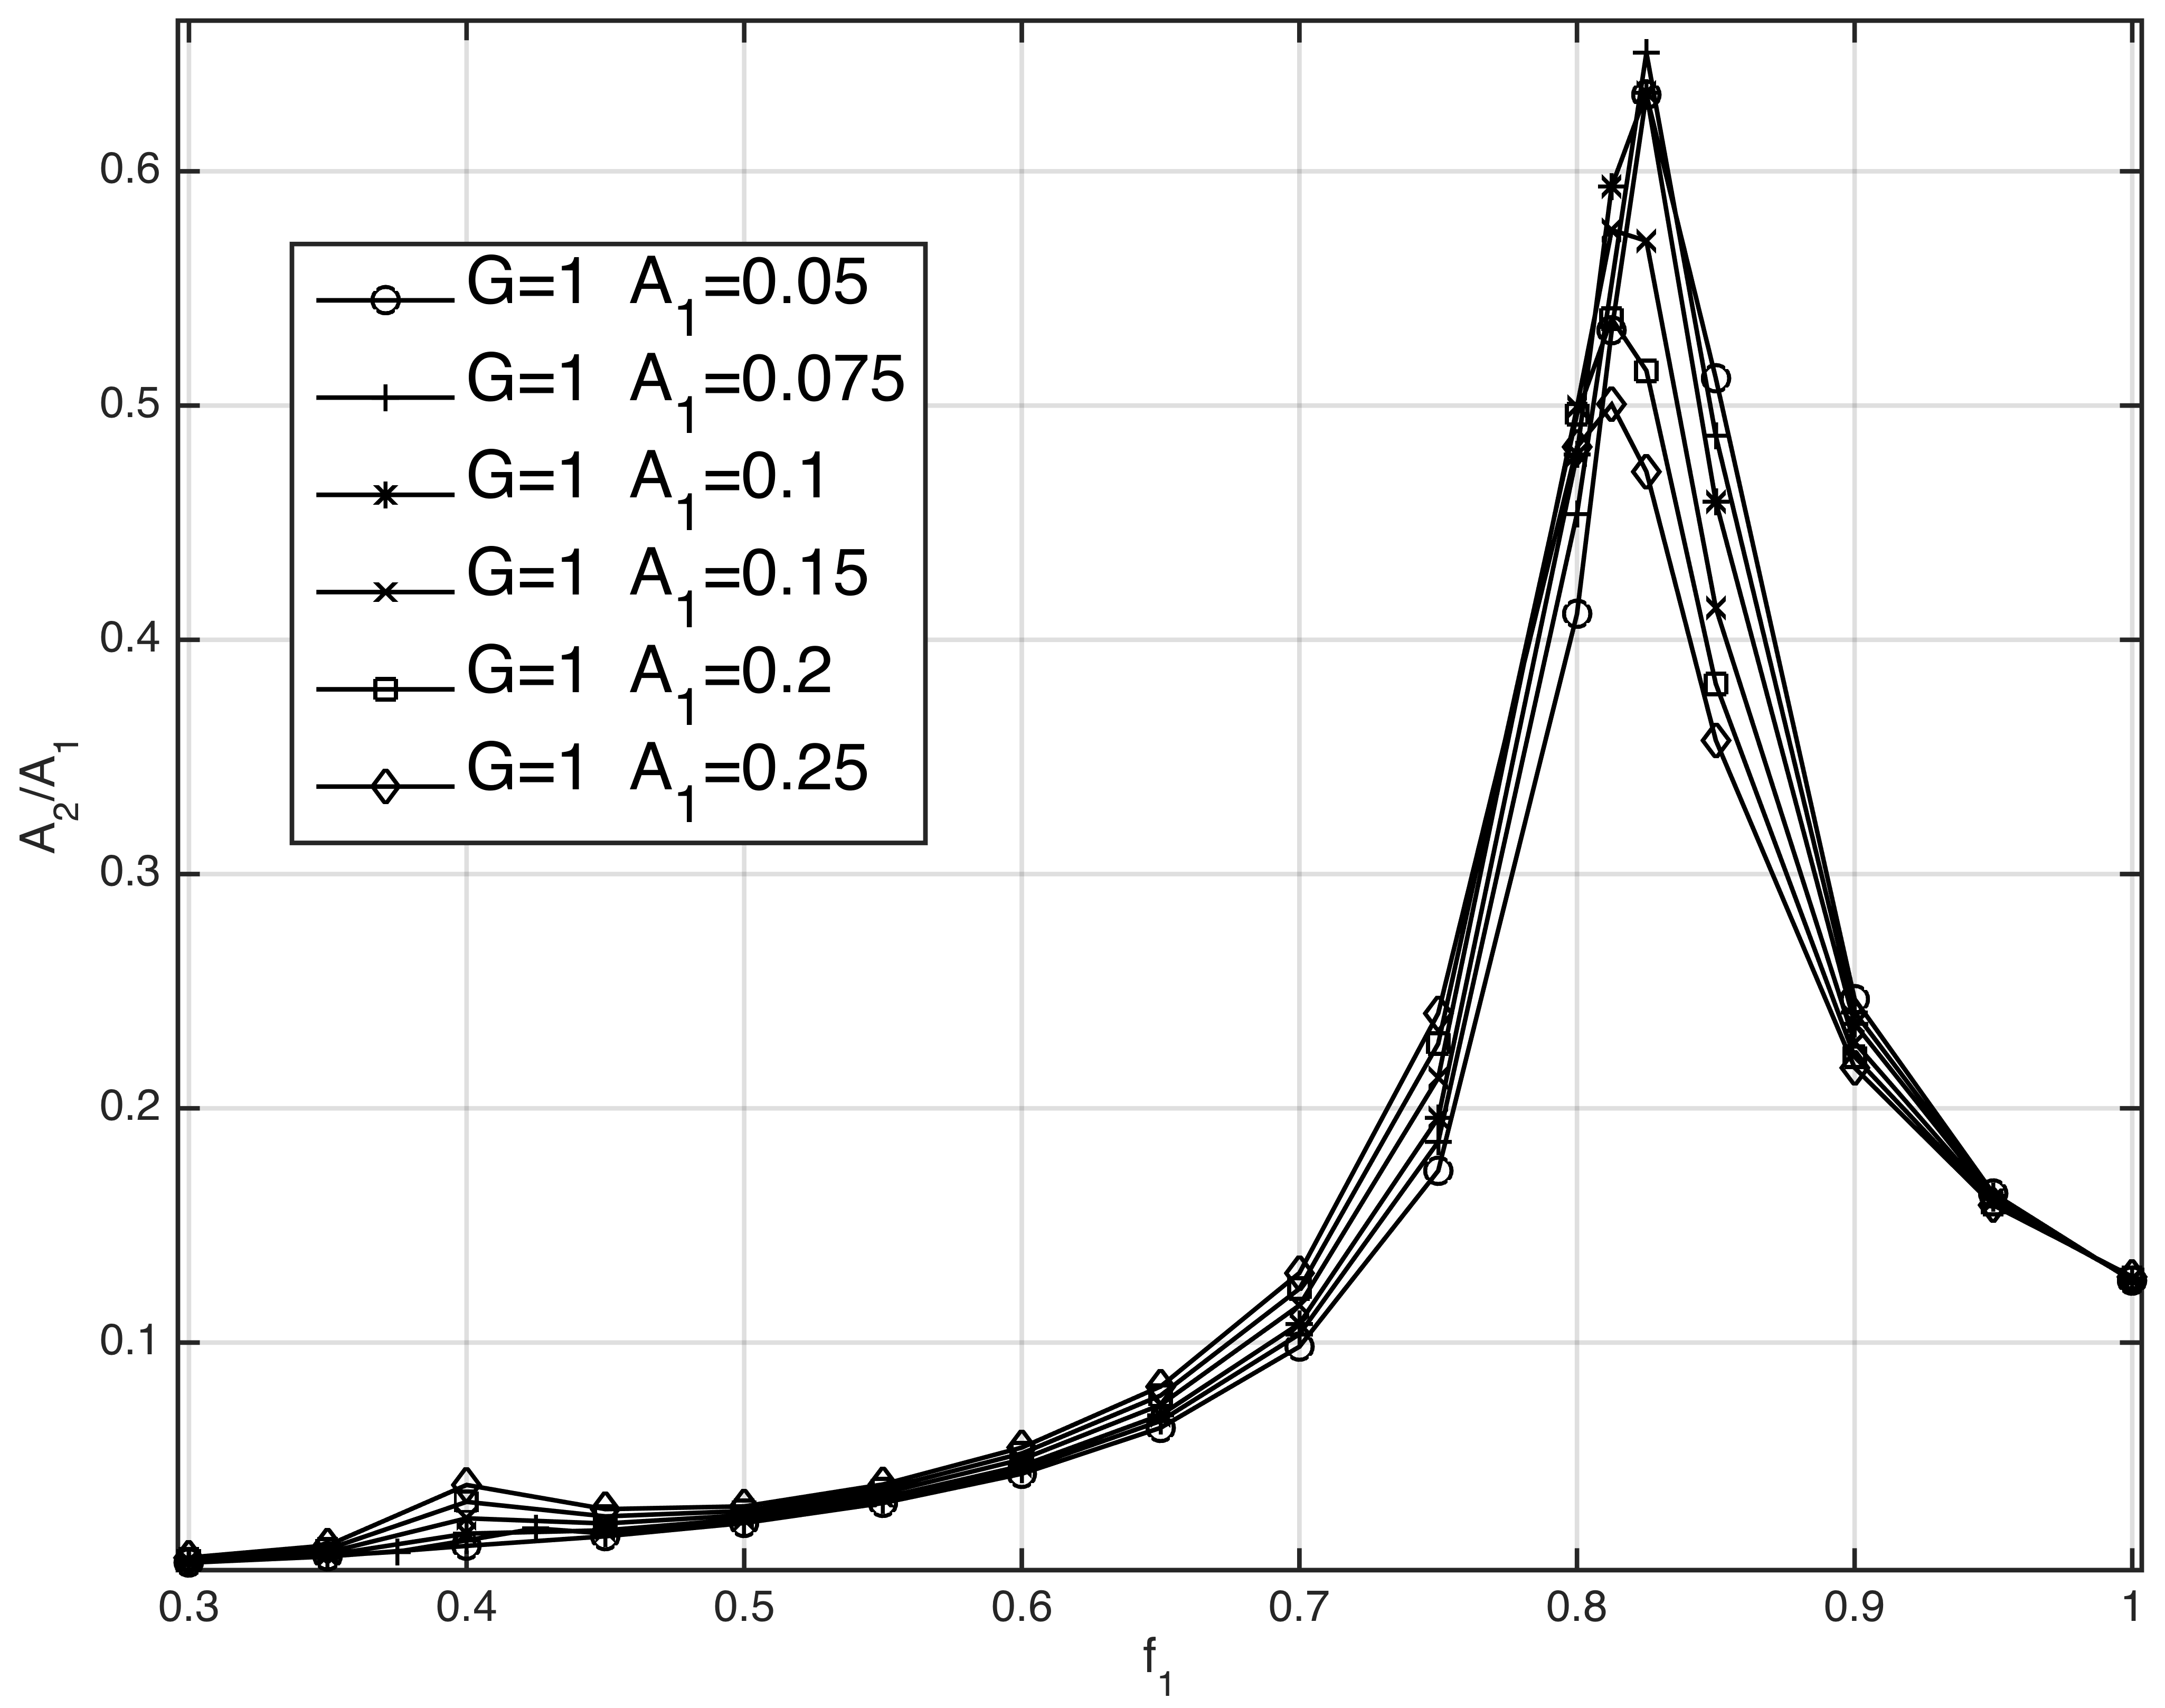
\includegraphics[width=\linewidth]{Figs/G=1_A2dA1}
		\caption{$ G=1 $, overview}
		\label{fig:g1a2da1}
	\end{subfigure}%
	\begin{subfigure}[t]{\widthp\textwidth}
		\centering
		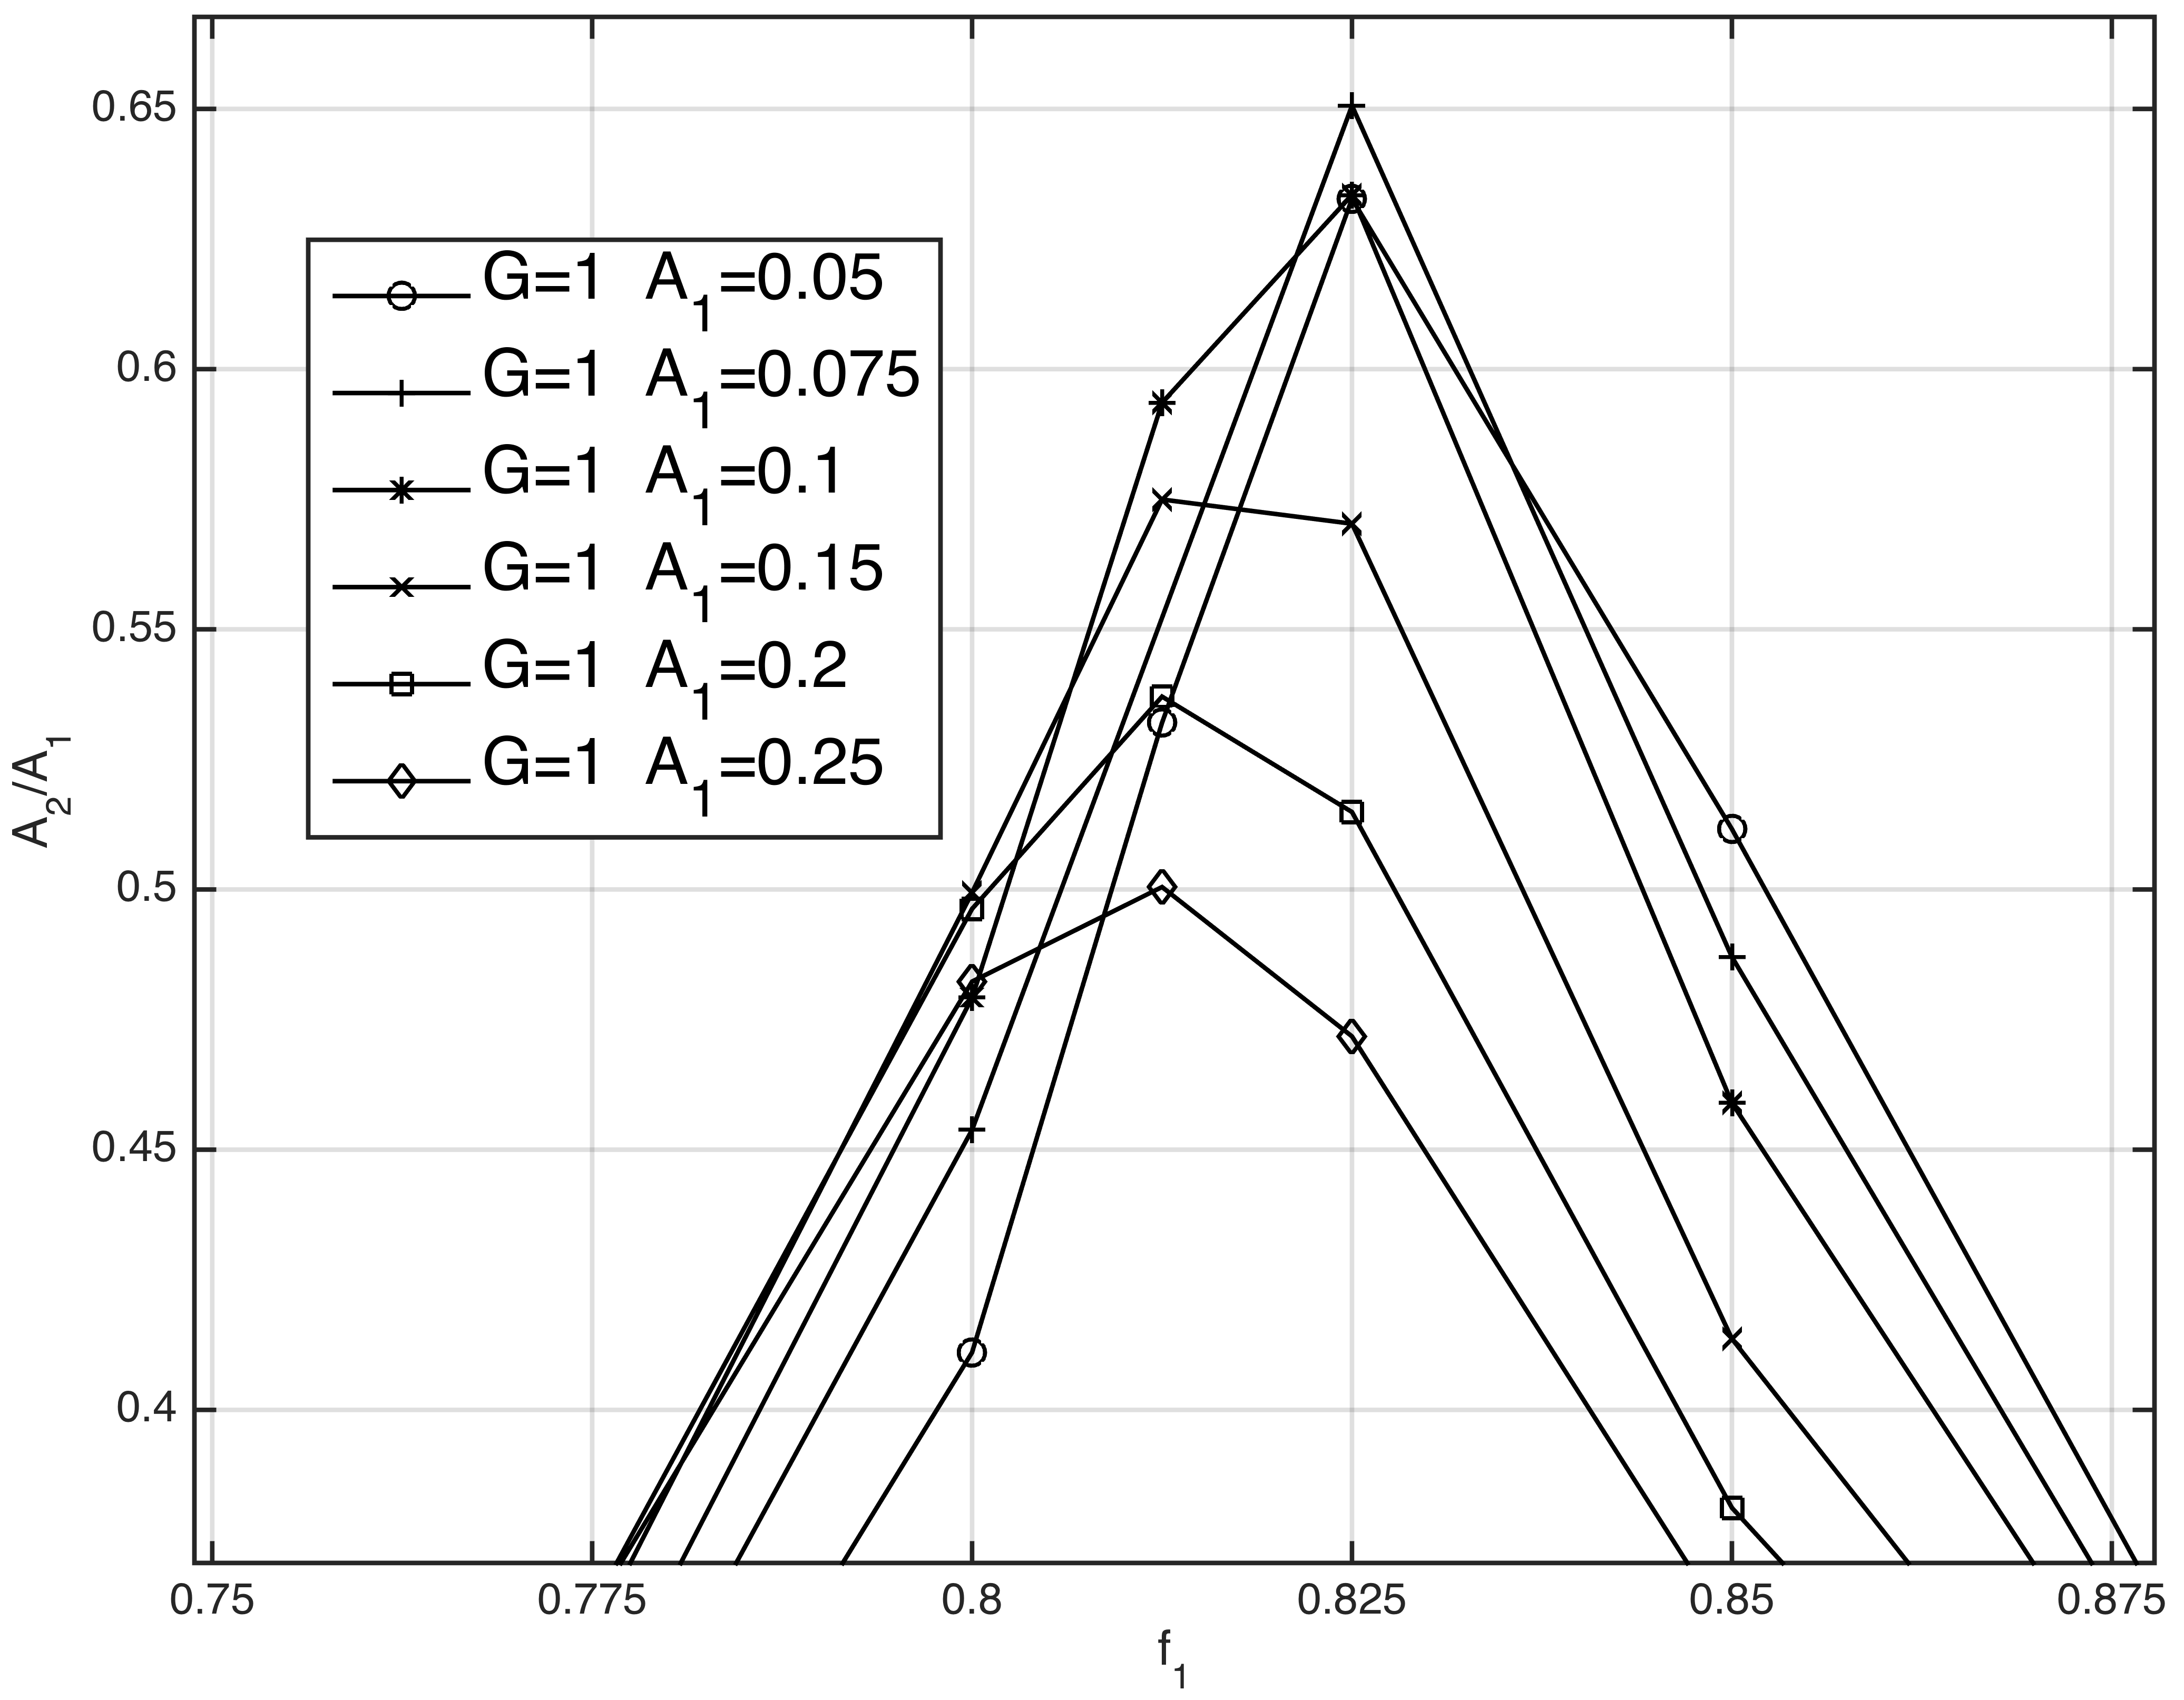
\includegraphics[width=\linewidth]{Figs/G=1_A2dA1_details}
		\caption{$ G=1 $, close-up}
		\label{fig:g1a2da1details}
	\end{subfigure}\\%
	\begin{subfigure}[t]{\widthp\textwidth}
		\centering
		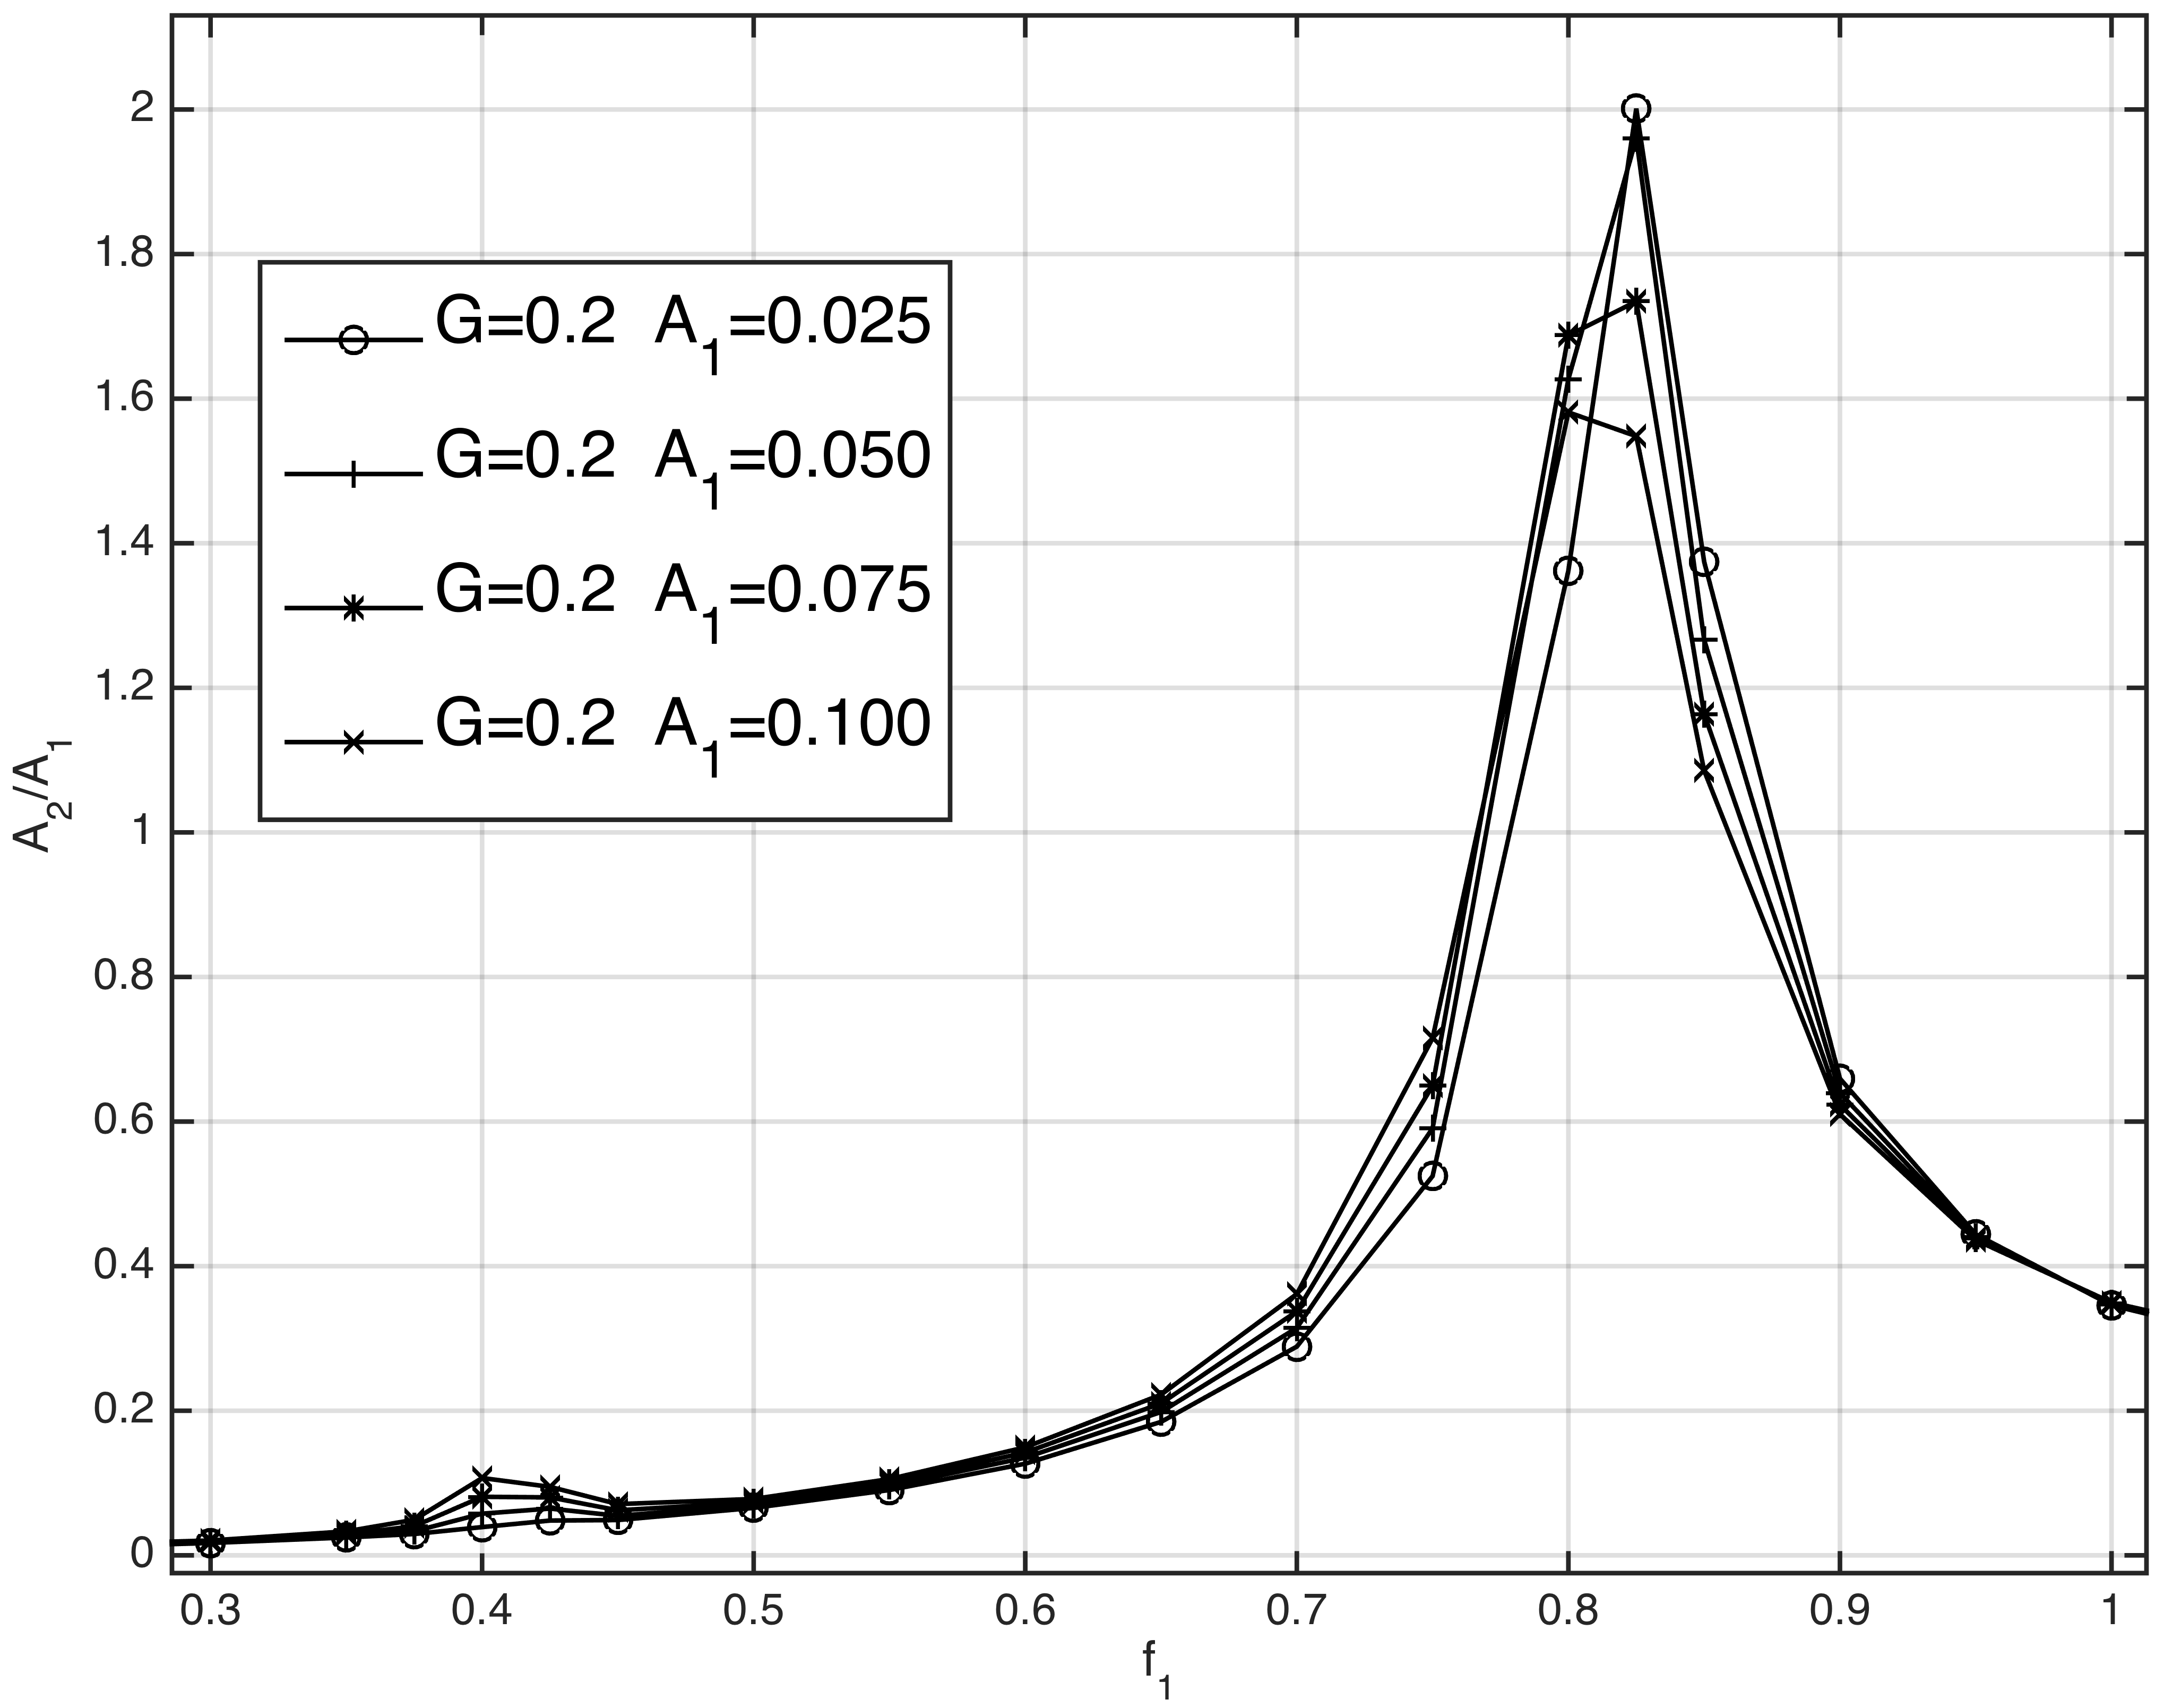
\includegraphics[width=\linewidth]{Figs/G=0.2_A2dA1}
		\caption{$ G=0.2 $, overview}
		\label{fig:g0.2A2dA1}
	\end{subfigure}%
	\begin{subfigure}[t]{\widthp\textwidth}
		\centering
		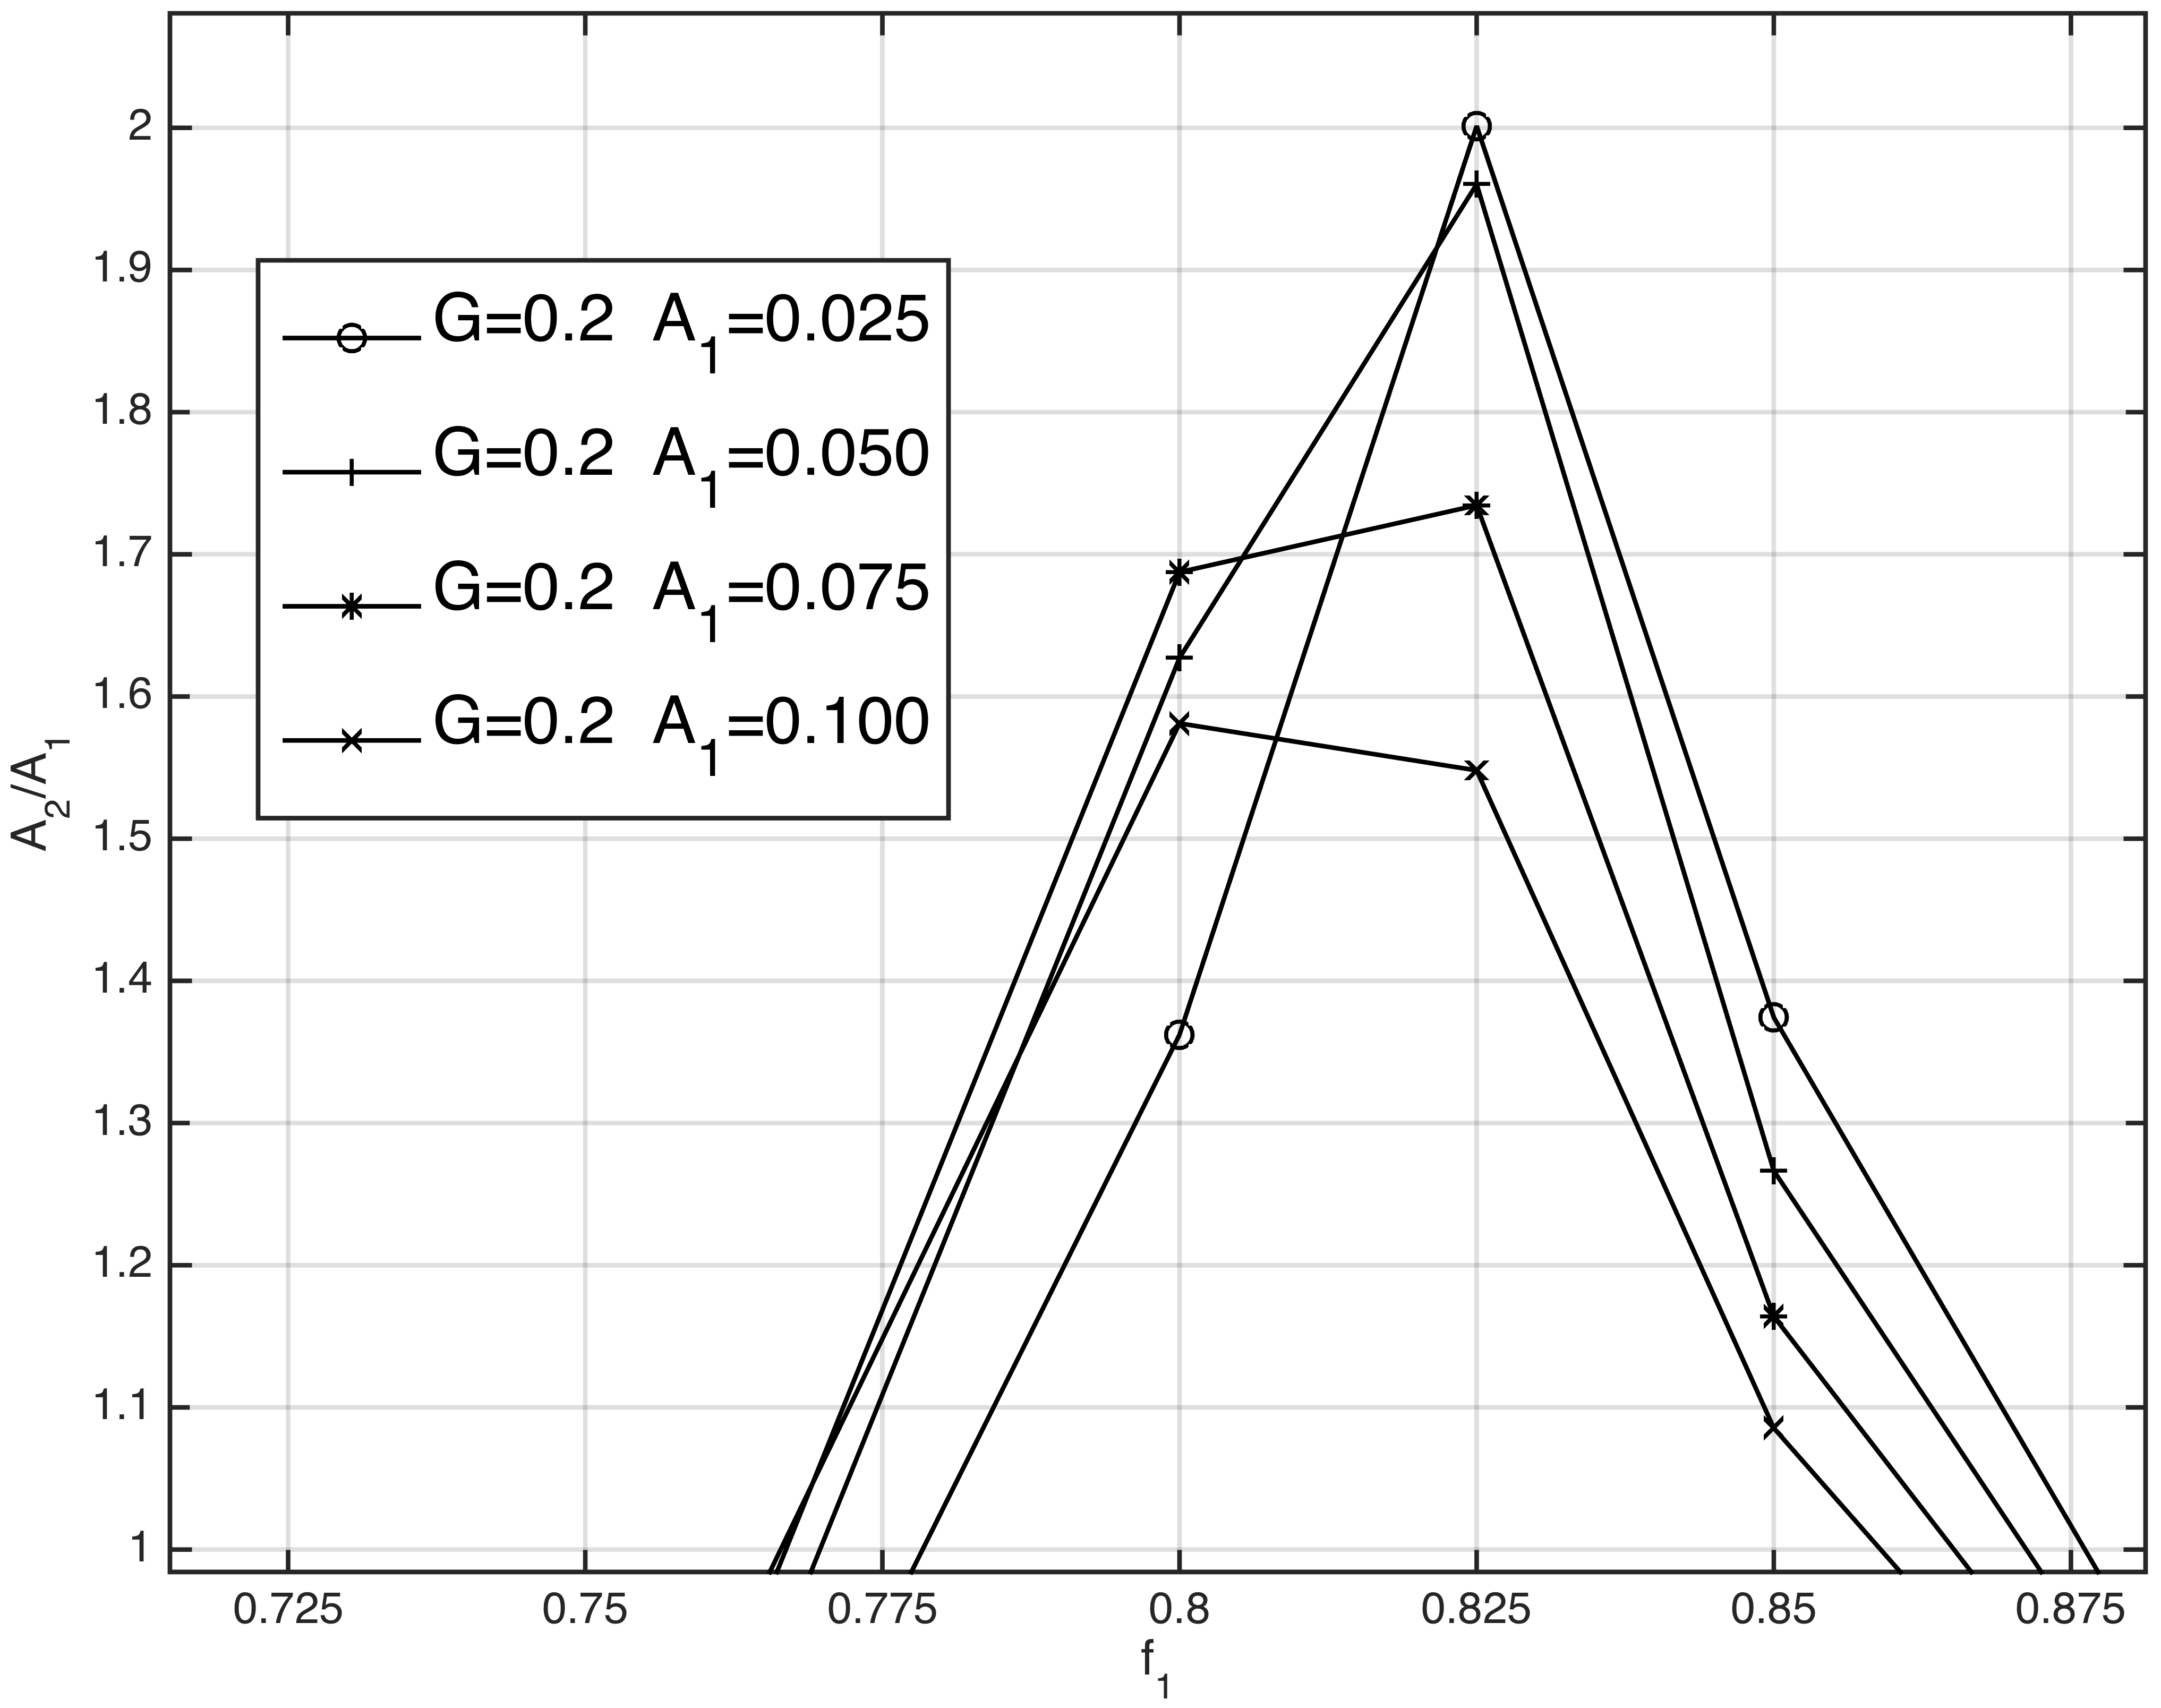
\includegraphics[width=\linewidth]{Figs/G=0.2_A2dA1_details}
		\caption{$ G=0.2 $, close-up}
		\label{fig:g0.2A2dA1details}
	\end{subfigure}%		
	\caption{
		(a) \& (c) \& (e) Variation of C2's amplification factor with the frequency of C1, for $G=0.2,\ 1$, 1.25; $A_1=$ 0.025, 0.05, 0.075, 0.1, 0.15, 0.2, 0.25, 1. (b) \& (d) \& (f) Close-up view near resonance. 
	}
		\label{fig:A2dA1}
\end{figure}

In \Cref{fig:g3,fig:A2dA1}, the maximum values of $A_2/A_1$ are always found to occur at around $ f_1 $=0.8, rather than $ f_1 $=1, which is because at low mass ratios the natural frequency of the structural in the fluid is less than the structural natural frequency \cite{Zhao2013}. The increase of $ A_1 $ leads to the reduction of the peak value of $ A_2/A_1 $ and the decrease in the resonance frequency. 

In terms of amplitude amplification, \Cref{fig:g0.2A2dA1,fig:g0.2A2dA1details} demonstrates the change in C2's amplitude $ (A_2/A_1) $ with the frequency of C1, with $ G=0.2 $ and $ A_1=0.05 $, 0.1. It is notable that the value of $ A_2/A_1 $ goes beyond 1.0 at $ f_1=0.8 $, meaning the consequent amplitude of C2 is greater than the input amplitude of C1. Moreover, \Cref{fig:gvsa2da1} shows the variation of peak values for $ A_2/A_1 $ with respect to $ G $. It can be seen that $ A_2/A_1 $ is above 1.0 when $ G\leq0.4 $, and stays almost constant when $ G\leq0.2 $.

In addition, the shift of vibration centre was observed in the cases with $ G =3$. Sometimes, the displacement of the vibration centre was even larger than the amplitude of the vibration. When $ G =3$, $ A_1 =1.0 \sim 2.5$ with increment of 0.5, and $ \fone=0.05\sim2.5 $ with increment of 0.05, the contour in \Cref{fig:contourdeltaydividedbya2gis3} shows combination of $ f_1 $ and $ A_1 $ for vibration centre displacement $\Delta\overline{Y}=A_2$. For the area above the red line (i.e. large $ f_1 $ and $ A_1 $), the vibration centre displacement becomes greater than the induced vibration amplitude $ A_2 $ and eventually exceeds 14 times of $ A_2 $ for the combination of greatest $ A_1 $ \& $ f_1 $. 
%The $\Delta\overline{Y}/A_2$ is always less than 1.0 for the case with $ G =3$ and $ A_1=0.5$.

Some examples of vibration centre shift are shown in \Cref{fig:centreshift}. \Cref{fig:centreshift01} depicts examples of C2's displacement histories for $ G=3.0 $, $A_{1}=0.5$, 1.0, 1.5, 2.0, and $f_{1}=2.5$. As the amplitude of C1 increases, the vibration centre of C2 keeps moving away from C1. A sudden drop of vibration centre from $+0.4$ to $-0.35$ occurs at $5\leq tf_{n}\leq 7$ and $A_{1}=2.0$. After the sudden drop, the vibration centre of C2 remains steady at -0.35, which is closer to C1 than at the start of the simulation. \Cref{fig:centreshift02} shows examples of C2's displacement histories for $ G=3.0 $, ${A}_{1}$=2.0, $\fone$=0.8, 2.0, 2.5. As frequency rises, the magnitude of C2's vibration centre shift becomes more apparent. While the vibration centre for $f_{1}=0.8$ remains constant at about $ +0.05 $, an abrupt decrease occurs for $f_{1}=2.0$ and 2.5. Although the vibration amplitude at $f_{1} = 2.0$ and 2.5 is smaller than that of $f_{1} = 0.8$, the vibration centre shift at these larger frequencies are much greater than the vibration amplitude. 
\begin{figure}[tbp]
	\centering
	\captionsetup{justification=centering}
	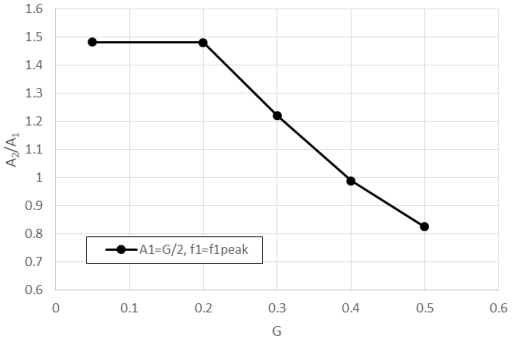
\includegraphics[width=0.65\linewidth]{Figs/GvsA2dA1}
	\caption{Variation of maximum $ A_2/A_1 $ with the gap ratio $ G $, where the value of $ A_1 $ is always $ G/2 $.}
	\label{fig:gvsa2da1}
\end{figure}
%done TD one more figure for frequency check
\begin{figure}[tbh!]	
	\newcommand\widthp{0.5}
	\centering
	\captionsetup{justification=centering}
	%\captionsetup[subfigure]{labelsep = none}
	%\captionsetup[subfigure]{labelformat = empty}
	\hspace*{\fill}%
	\begin{subfigure}[t]{\widthp\textwidth}
		\centering
		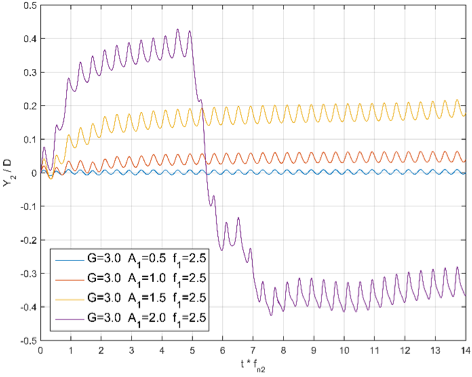
\includegraphics[width=\linewidth]{Figs/centreshift01}
		\caption{$G=3.0$, $f_1=2.5$, $A_1=0.5$, 1.0, 1.5, 2.0}
		\label{fig:centreshift01}
	\end{subfigure}%
	\begin{subfigure}[t]{\widthp\textwidth}
		\centering
		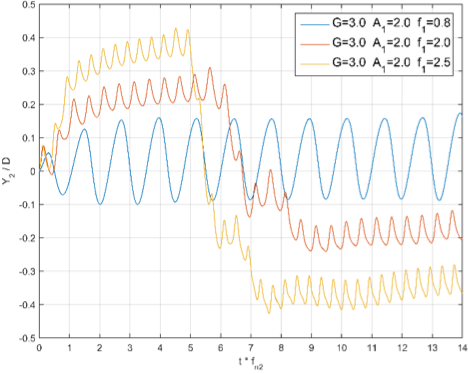
\includegraphics[width=\linewidth]{Figs/centreshift02}
		\caption{$G=3.0$, $A_1=2.0$, $f_1=0.8$, 2.0, 2.5}
		\label{fig:centreshift02}
	\end{subfigure}%
	\caption{
		Displacement time histories of C2
	}
	\label{fig:centreshift}
\end{figure}



%TD explain why resonance occurs at around 0.8fn


\clearpage
\section{Discussion} \label{sec discussion}
For all the cases simulated (see \Cref{fig:A2dA1}), major resonance occurs when $ \widetilde{f}_1=0.8 $. That is because $ f_{wn}/f_n=\sqrt{m^*/(m^*+C_A)} $. Also, $ C_A $ of a cylinder can be approximated as 1.273\cite{Techet2005c}, which means $ f_{wn}/f_n=0.814 $. This explains the large resonance peak at 80 percent structural natural frequency.

%TD something wrong with Plotting_g3.0a1.5m2.5_01.35_VIV02.png

\section{Summary} \label{sec interconlude}
%aTD: the previous conlusion may need to be changed

Using numerical simulations, we investigated the mechanical interactions between two submerged cylinders. The active cylinder C1 underwent forced vibration with specified amplitude and frequency. All the cases studied had constant Reynolds number of 100 and mass ratio of 2.5. The passive cylinder C2 responded to the oscillation of the active cylinder by way of the induced fluid motion in the following way: 
\begin{enumerate}
	\item The amplitude of C2 reached its maximum when the frequency of C1 was close to 80\% of the C2's structural natural frequency ($ f_n $). 
	\item The increase of C1's amplitude led to the rise of C2's amplitude, but the decrease of the amplitude magnification factor ($ A_2/A_1 $) and the slight decrease of the resonance frequency.
	\item The vibration centre of C2 shifted away from the initial location for cases with $ \widetilde{G}/D=3 $, and the shift became increasingly obvious with the increase of $ A_1 $ and $ f_1 $.
	\item For cases with $ A_1=G/2 $, the values of maximum $ A_2/A_1 $ were above 1.0, at $ G<0.4 $.
\end{enumerate}
\begin{figure}[tbp]
	\centering
	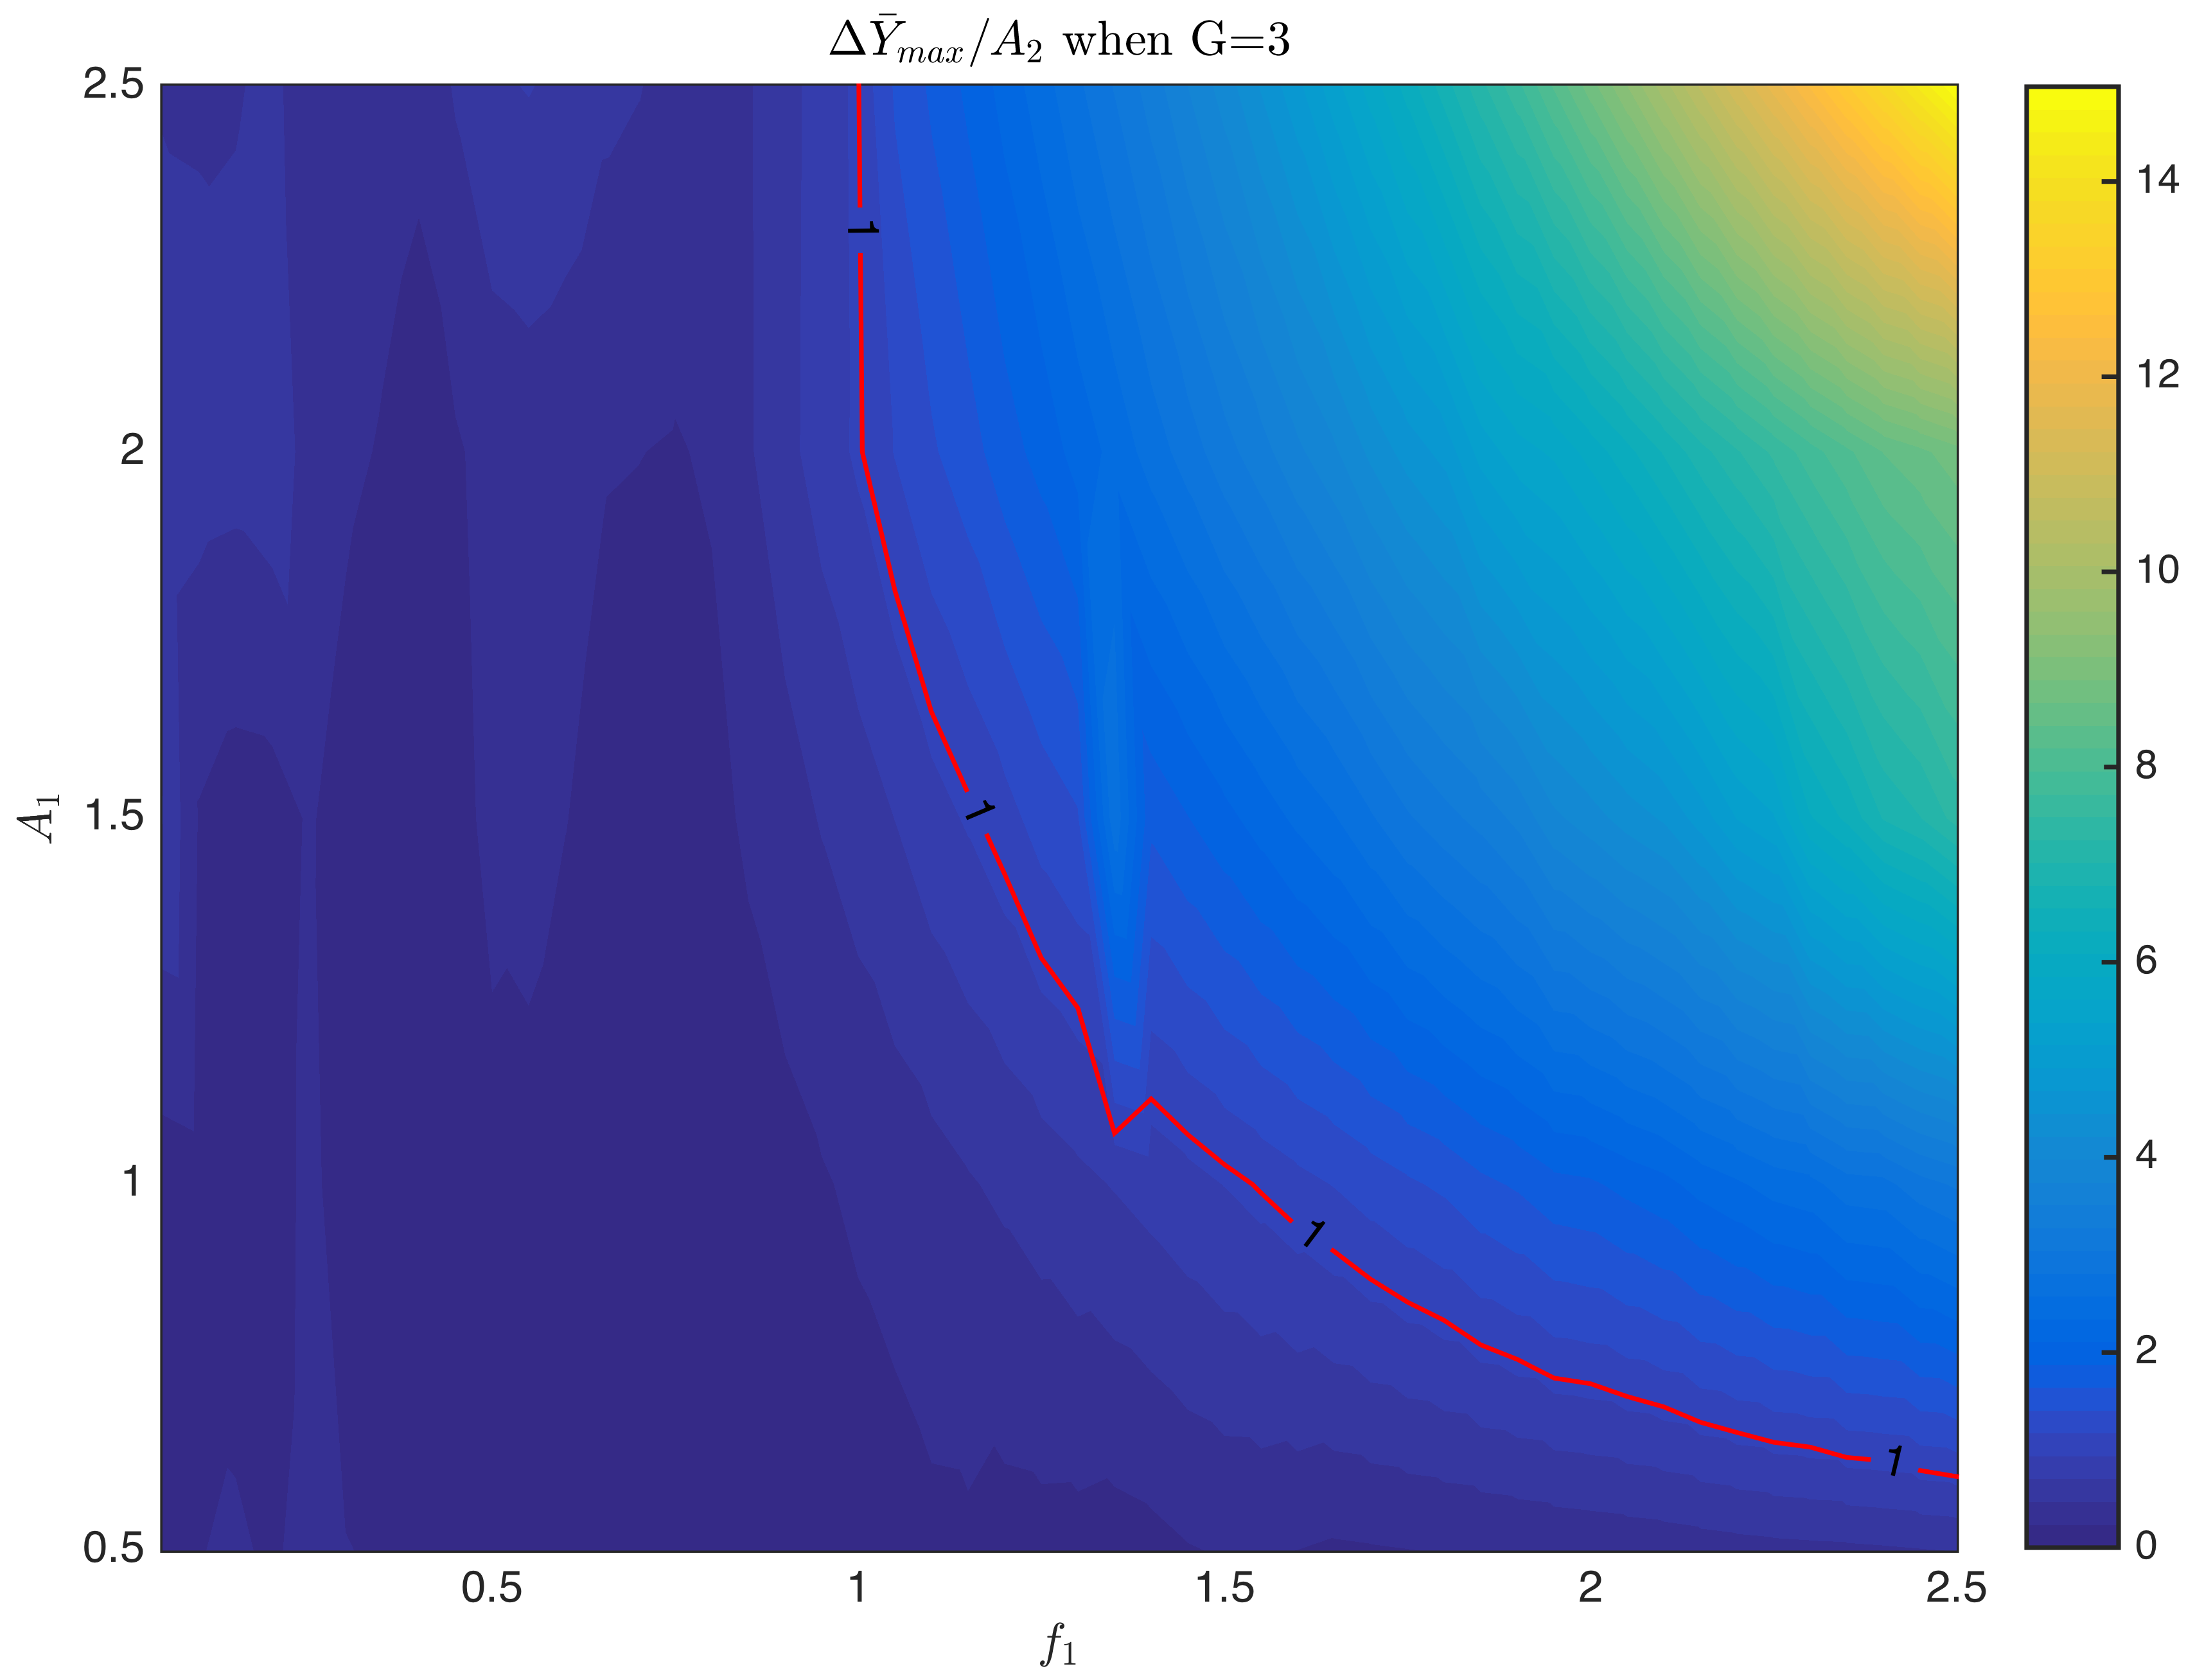
\includegraphics[width=0.85\linewidth]{Figs/Contour_deltaY_divided_by_A2_G_is_3}
	\caption{
		Dependence of $\Delta\overline{Y}/A_2$ on $A_1$ \& $f_1 $for $ G $=3
	}
	\label{fig:contourdeltaydividedbya2gis3}
\end{figure}


%\begin{figure}[tbp]	
%	\newcommand\widthp{0.5}
%	\centering
%	\captionsetup{justification=centering}
%	%\captionsetup[subfigure]{labelsep = none}
%	%\captionsetup[subfigure]{labelformat = empty}
%	\hspace*{\fill}%
%	\begin{subfigure}[t]{\widthp\textwidth}
%		\centering
%		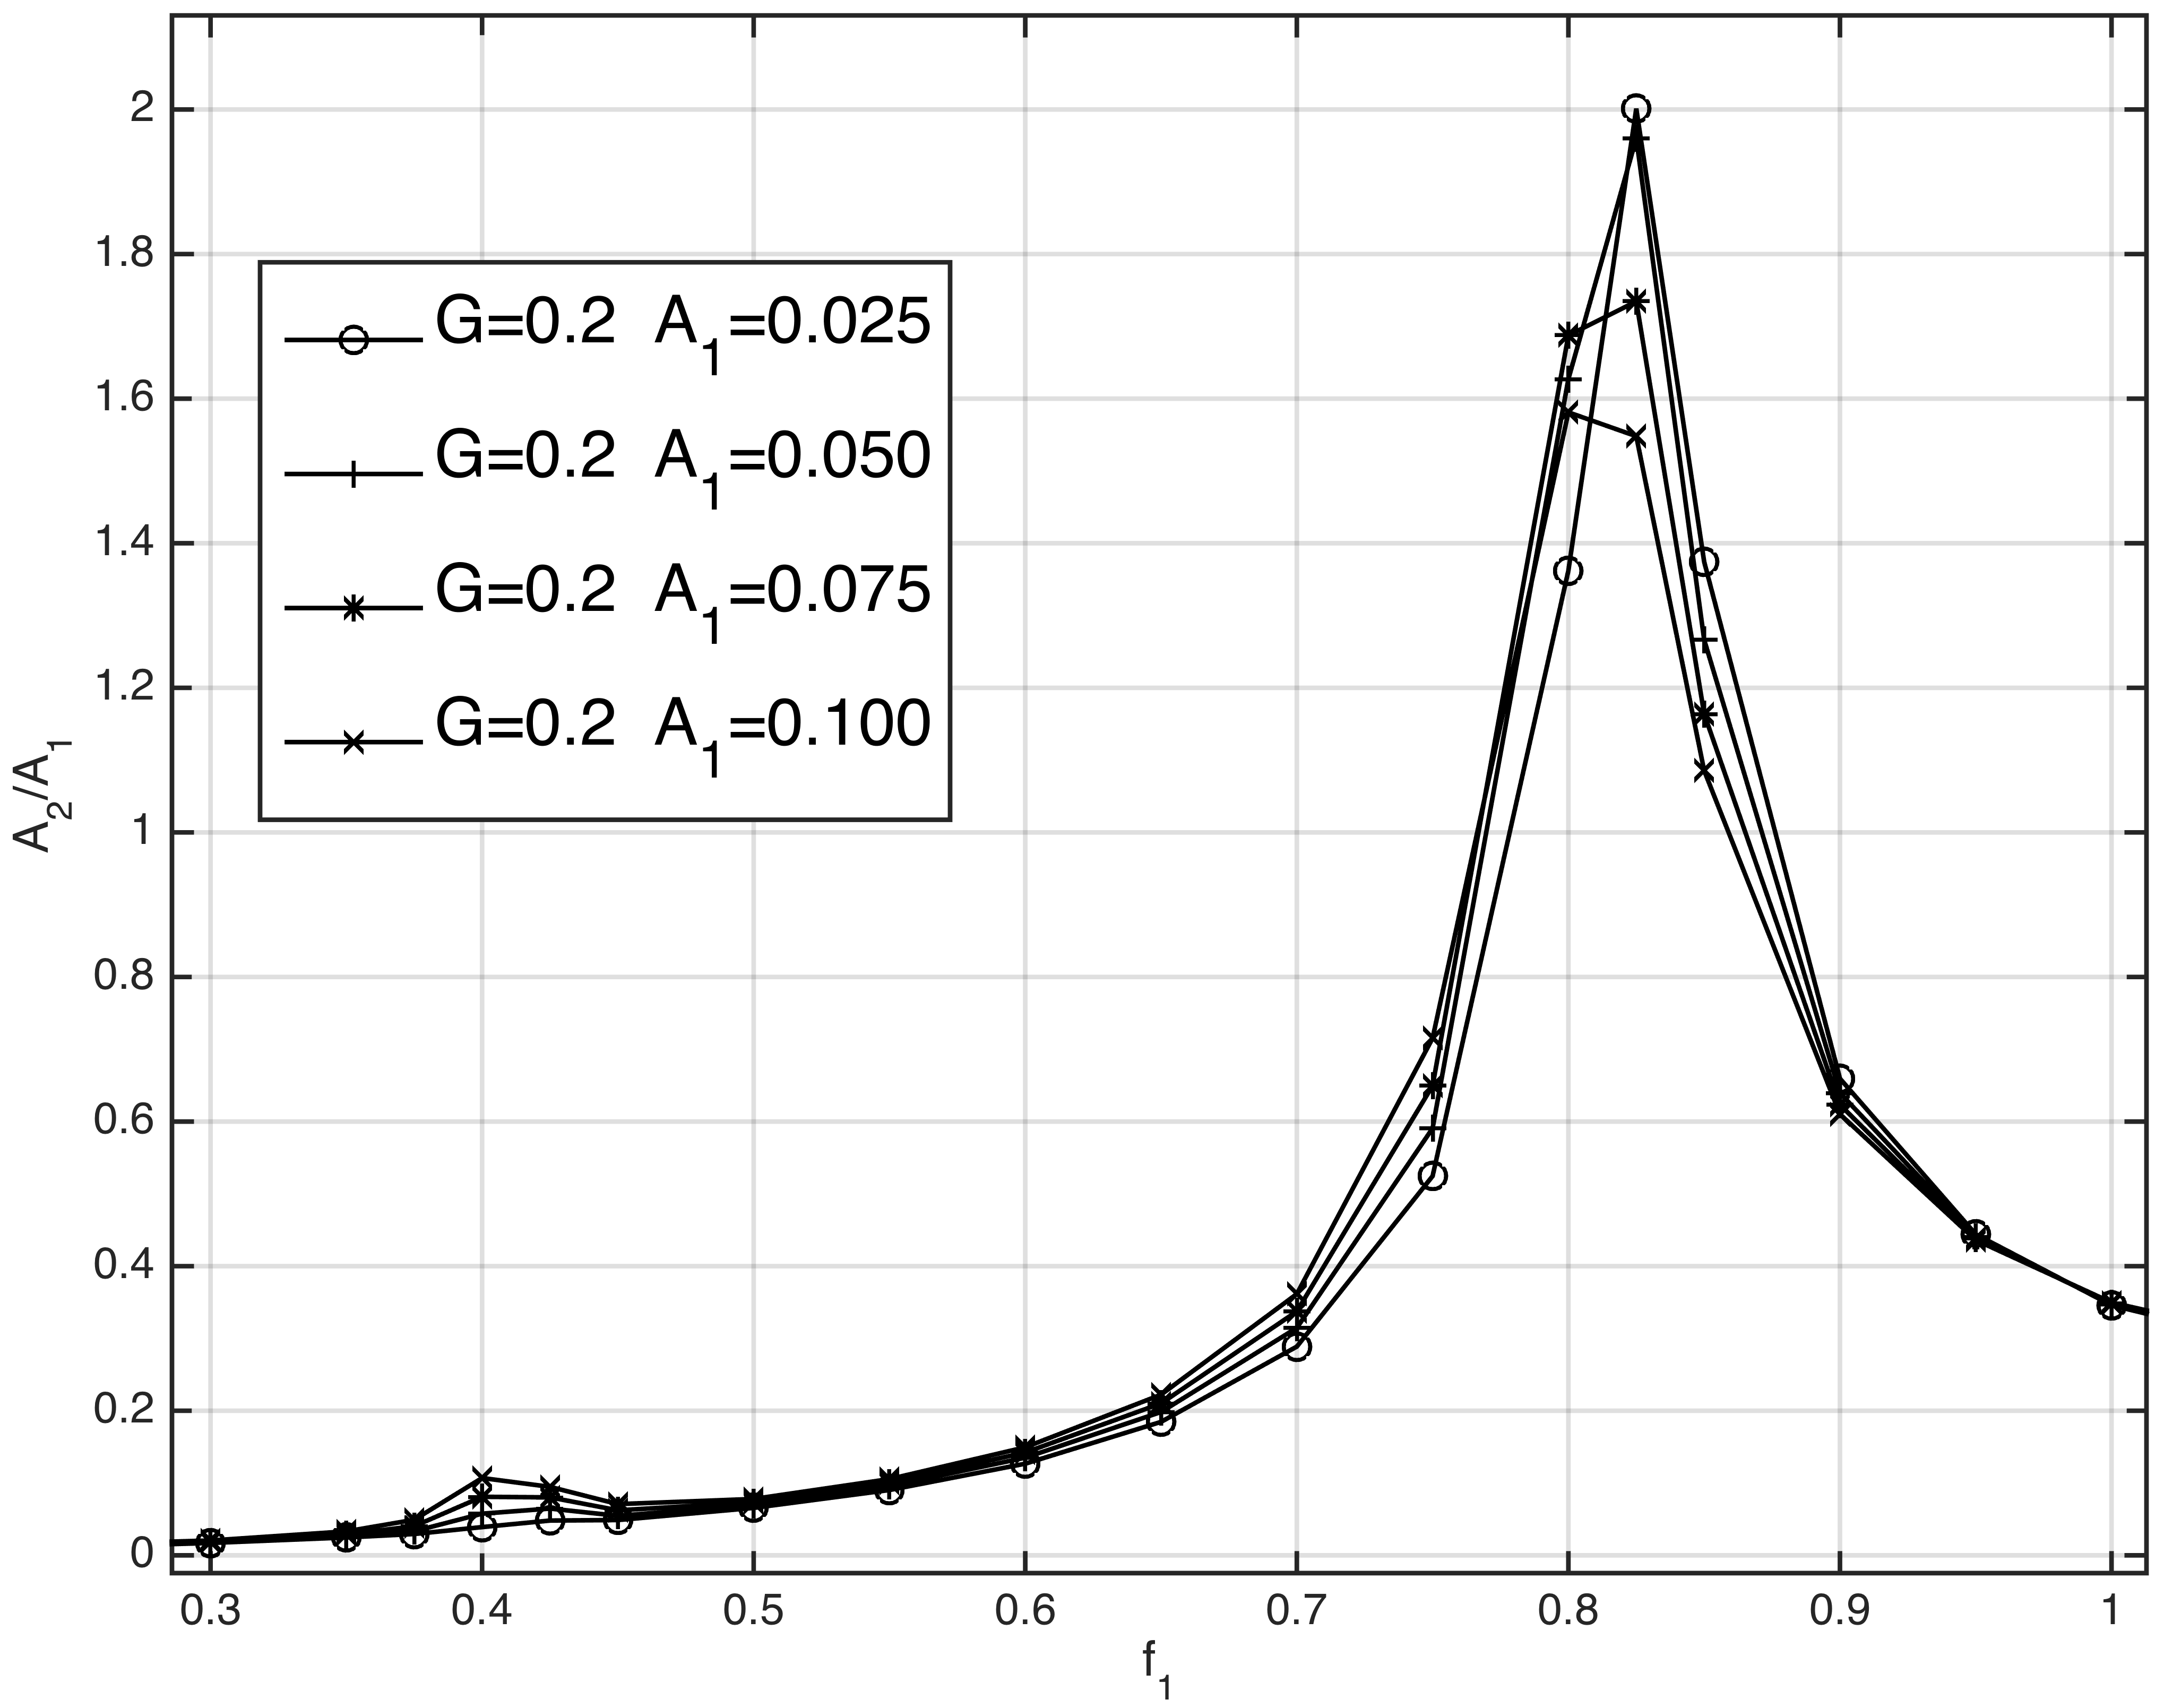
\includegraphics[width=\linewidth]{Figs/G=0.2_A2dA1}
%		\caption{$ G=0.2 $, overview}
%		\label{fig:g0.2A2dA1}
%	\end{subfigure}%
%	\begin{subfigure}[t]{\widthp\textwidth}
%		\centering
%		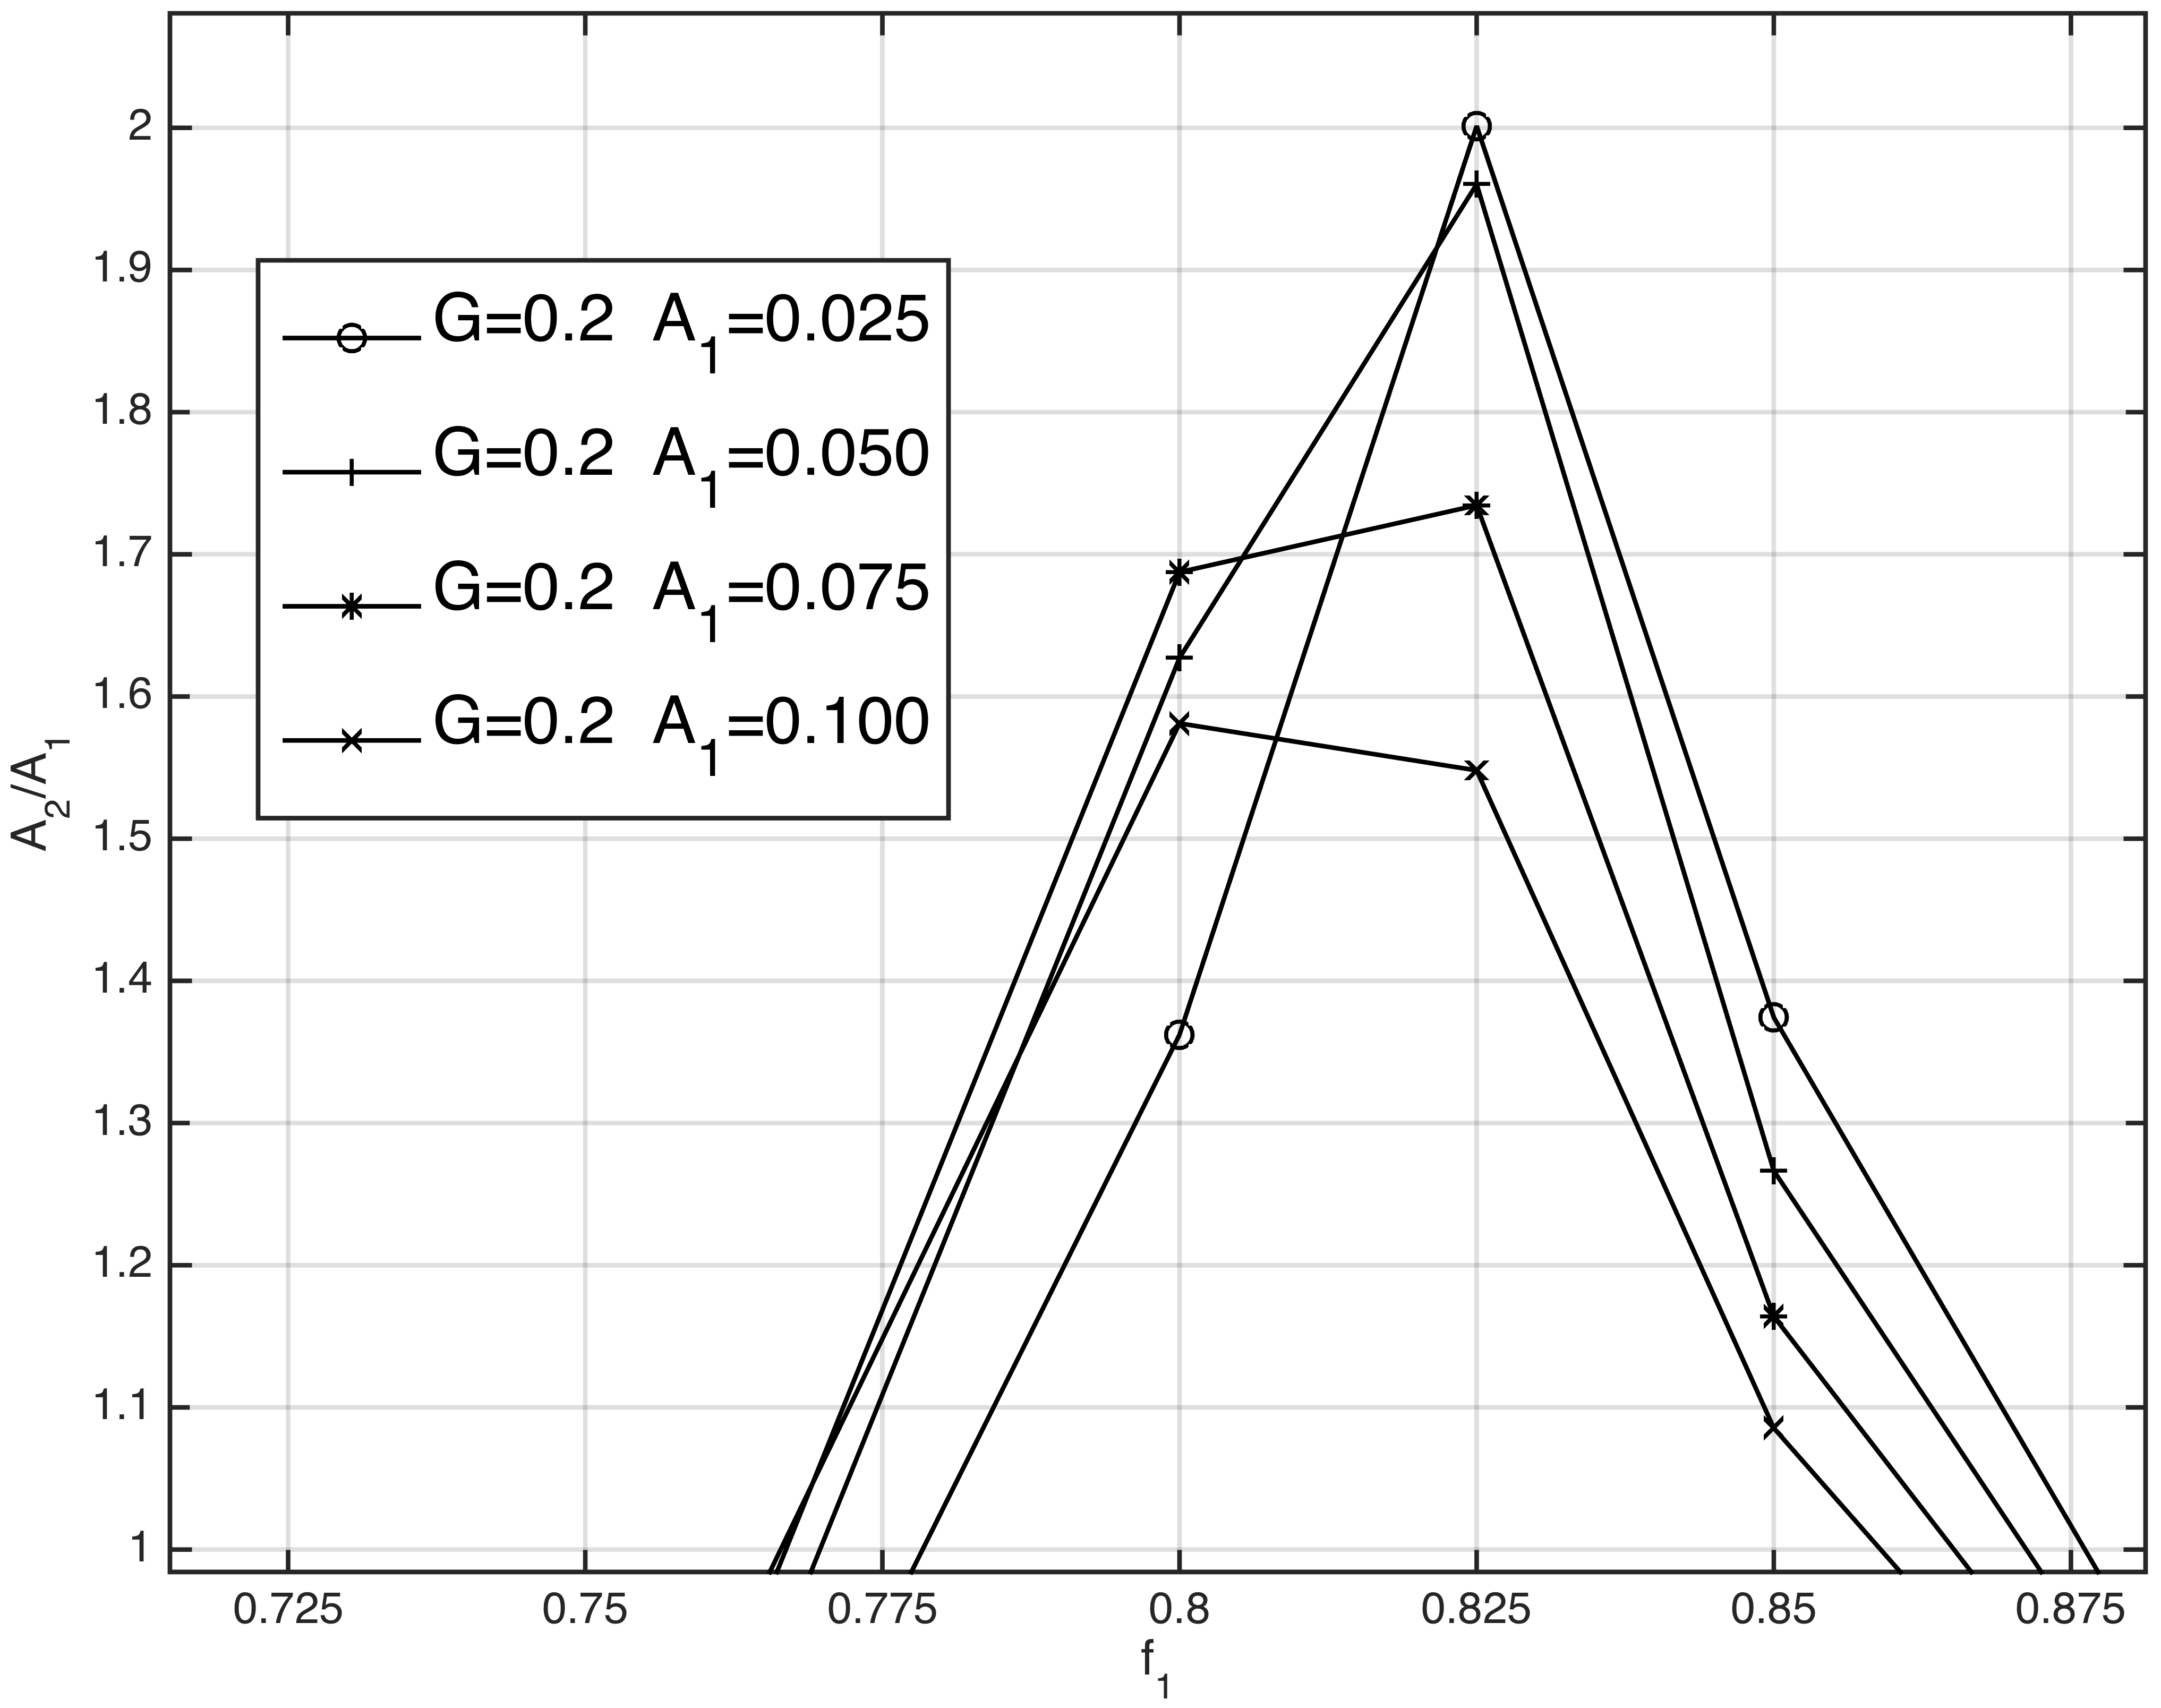
\includegraphics[width=\linewidth]{Figs/G=0.2_A2dA1_details}
%		\caption{$ G=0.2 $, close-up}
%		\label{fig:g0.2A2dA1details}
%	\end{subfigure}%
%	\caption{
%		Displacement time histories of C2 (a) for $G=3.0$, $f_1=2.5$, $A_1=0.5$, 1.0, 1.5, 2.0. (b) for $G=3.0$, $A_1=2.0$, $f_1=0.8$, 2.0, 2.5.
%	}
%	\label{fig:g0.2}
%\end{figure}






%relationship between vortex pattern and vibration
%phase of vortex
%Add Forces' plotting


%\section{Resonance}
%
%\section{Amplitude amplification}
%
%\section{Vibration centre shift}


%\begin{table}
%\caption{A nice looking table}
%\centering
%\label{table:nice_table}
%\begin{tabular}{l c c c c}
%\hline 
%\multirow{2}{*}{Dental measurement} & \multicolumn{2}{c}{Species I} & \multicolumn{2}{c}{Species II} \\ 
%\cline{2-5}
%  & mean & SD  & mean & SD  \\ 
%\hline
%I1MD & 6.23 & 0.91 & 5.2  & 0.7  \\
%
%I1LL & 7.48 & 0.56 & 8.7  & 0.71 \\
%
%I2MD & 3.99 & 0.63 & 4.22 & 0.54 \\
%
%I2LL & 6.81 & 0.02 & 6.66 & 0.01 \\
%
%aCMD & 13.47 & 0.09 & 10.55 & 0.05 \\
%
%aCBL & 11.88 & 0.05 & 13.11 & 0.04\\ 
%\hline 
%\end{tabular}
%\end{table}
%
%
%\begin{table}
%\caption{Even better looking table using booktabs}
%\centering
%\label{table:good_table}
%\begin{tabular}{l c c c c}
%\toprule
%\multirow{2}{*}{Dental measurement} & \multicolumn{2}{c}{Species I} & \multicolumn{2}{c}{Species II} \\ 
%\cmidrule{2-5}
%  & mean & SD  & mean & SD  \\ 
%\midrule
%I1MD & 6.23 & 0.91 & 5.2  & 0.7  \\
%
%I1LL & 7.48 & 0.56 & 8.7  & 0.71 \\
%
%I2MD & 3.99 & 0.63 & 4.22 & 0.54 \\
%
%I2LL & 6.81 & 0.02 & 6.66 & 0.01 \\
%
%aCMD & 13.47 & 0.09 & 10.55 & 0.05 \\
%
%aCBL & 11.88 & 0.05 & 13.11 & 0.04\\ 
%\bottomrule
%\end{tabular}
%\end{table}

%==================

